\documentclass[%
    fontsize=12pt,
    headinclude,
    paper=a4,
    numbers=noenddot,
    listof=totoc,
    bibliography=totoc,
    index=totoc,
]{diplomarbeit}

\areaset[20mm]{160mm}{240mm}	% Binderand, Breite und Höhe nutzbarer Bereich
% \usepackage[textwidth=160mm,textheight=240mm]{geometry}

\usepackage{amssymb,amsmath}

\usepackage{color}
\usepackage{fancyvrb}

% bright ansi colors
\definecolor{darkgray}{gray}{0.25}
\definecolor{lightred}{rgb}{1.0,0.39,0.28}
\definecolor{lightgreen}{rgb}{0.48,0.99,0.0}
\definecolor{lightblue}{rgb}{0.53,0.81,0.92}
\definecolor{lightpurple}{rgb}{0.87,0.63,0.87}
\definecolor{lightcyan}{rgb}{0.5,1.0,0.83}

% commands and environments needed by pandoc snippets
% extracted from the output of `pandoc -s`
\providecommand{\tightlist}{%
  \setlength{\itemsep}{0pt}\setlength{\parskip}{0pt}}
\DefineVerbatimEnvironment{Highlighting}{Verbatim}{commandchars=\\\{\}}
% Add ',fontsize=\small' for more characters per line
\newenvironment{Shaded}{}{}
\newcommand{\KeywordTok}[1]{\textcolor[rgb]{0.00,0.44,0.13}{\textbf{{#1}}}}
\newcommand{\DataTypeTok}[1]{\textcolor[rgb]{0.56,0.13,0.00}{{#1}}}
\newcommand{\DecValTok}[1]{\textcolor[rgb]{0.25,0.63,0.44}{{#1}}}
\newcommand{\BaseNTok}[1]{\textcolor[rgb]{0.25,0.63,0.44}{{#1}}}
\newcommand{\FloatTok}[1]{\textcolor[rgb]{0.25,0.63,0.44}{{#1}}}
\newcommand{\CharTok}[1]{\textcolor[rgb]{0.25,0.44,0.63}{{#1}}}
\newcommand{\StringTok}[1]{\textcolor[rgb]{0.25,0.44,0.63}{{#1}}}
\newcommand{\CommentTok}[1]{\textcolor[rgb]{0.38,0.63,0.69}{\textit{{#1}}}}
\newcommand{\OtherTok}[1]{\textcolor[rgb]{0.00,0.44,0.13}{{#1}}}
\newcommand{\AlertTok}[1]{\textcolor[rgb]{1.00,0.00,0.00}{\textbf{{#1}}}}
\newcommand{\FunctionTok}[1]{\textcolor[rgb]{0.02,0.16,0.49}{{#1}}}
\newcommand{\RegionMarkerTok}[1]{{#1}}
\newcommand{\ErrorTok}[1]{\textcolor[rgb]{1.00,0.00,0.00}{\textbf{{#1}}}}
\newcommand{\NormalTok}[1]{{#1}}



% Additional commands for more recent versions of Pandoc
\newcommand{\ConstantTok}[1]{\textcolor[rgb]{0.53,0.00,0.00}{{#1}}}
\newcommand{\SpecialCharTok}[1]{\textcolor[rgb]{0.25,0.44,0.63}{{#1}}}
\newcommand{\VerbatimStringTok}[1]{\textcolor[rgb]{0.25,0.44,0.63}{{#1}}}
\newcommand{\SpecialStringTok}[1]{\textcolor[rgb]{0.73,0.40,0.53}{{#1}}}
\newcommand{\ImportTok}[1]{{#1}}
\newcommand{\DocumentationTok}[1]{\textcolor[rgb]{0.73,0.13,0.13}{\textit{{#1}}}}
\newcommand{\AnnotationTok}[1]{\textcolor[rgb]{0.38,0.63,0.69}{\textbf{\textit{{#1}}}}}
\newcommand{\CommentVarTok}[1]{\textcolor[rgb]{0.38,0.63,0.69}{\textbf{\textit{{#1}}}}}
\newcommand{\VariableTok}[1]{\textcolor[rgb]{0.10,0.09,0.49}{{#1}}}
\newcommand{\ControlFlowTok}[1]{\textcolor[rgb]{0.00,0.44,0.13}{\textbf{{#1}}}}
\newcommand{\OperatorTok}[1]{\textcolor[rgb]{0.40,0.40,0.40}{{#1}}}
\newcommand{\BuiltInTok}[1]{{#1}}
\newcommand{\ExtensionTok}[1]{{#1}}
\newcommand{\PreprocessorTok}[1]{\textcolor[rgb]{0.74,0.48,0.00}{{#1}}}
\newcommand{\AttributeTok}[1]{\textcolor[rgb]{0.49,0.56,0.16}{{#1}}}
\newcommand{\InformationTok}[1]{\textcolor[rgb]{0.38,0.63,0.69}{\textbf{\textit{{#1}}}}}
\newcommand{\WarningTok}[1]{\textcolor[rgb]{0.38,0.63,0.69}{\textbf{\textit{{#1}}}}}



% Define a nice break command that doesn't care if a line doesn't already
% exist.
\def\br{\hspace*{\fill} \\* }
% Math Jax compatability definitions
\def\gt{>}
\def\lt{<}
% Document parameters
% \usepackage{subcaption}
% \expandafter\def\csname ver@subfig.sty\endcsname{}

\usepackage{bibgerm}		% Für geralpha.bst. MUSS vor babel stehen
\usepackage[utf8]{inputenc}	% Latin1 input encoding (umlauts)
\usepackage[ngerman,english]{babel}
\usepackage{csquotes}       % ensure that quotes are typeset in main language

 
\usepackage[
    backend=biber,
    style=numeric-comp,
    sorting=ynt
]{biblatex}
\addbibresource{mendeley.bib}


\usepackage{parskip}		% seperate paragraphs by skip (blank line)
%\usepackage{amsfonts,amsmath,amssymb,array} % choose if needed
%\usepackage{ae,aecompl}	% Benutze 'Almost European' Zeichensatz         
%\usepackage{type1cm}	% Computer Modern type 1 fonts
\usepackage{lmodern}	% Latin Modern nehmen, da mehr Glyphen vorhanden 
\usepackage[T1]{fontenc}	% Verwende T1-Kodierung für Zeichensätze        

\usepackage{textcomp} % to make ° work


\usepackage{changebar}
\usepackage{makeidx}\makeindex

\usepackage[table,dvipsnames,svgnames,x11names,hyperref]{xcolor}
\definecolor{ColorLink}{rgb}{0,0.4549,0.8510}
\colorlet{ColorAlternatedRow}{lightgray!25}
\definecolor{DiagramRed}{HTML}{B85450}
\definecolor{DiagramGreen}{HTML}{82B366}
\definecolor{DiagramBlue}{HTML}{6C8EBF}
\definecolor{DiagramGray}{HTML}{666666}


\usepackage{graphicx}
\graphicspath{{gfx/}{gfx/boards/}{gfx/diagrams/}{gfx/figures/}{gfx/logos/}{gfx/models/}{gfx/pictures/}{gfx/results/}{gfx/screenshots/}}
\usepackage[export]{adjustbox} % https://tex.stackexchange.com/a/124372/142289
\usepackage{svg}
\usepackage{mdframed}
\usepackage{subcaption}
\usepackage{calc}         % for \svgscale

% https://tex.stackexchange.com/questions/42619/x-mark-to-match-checkmark
\usepackage{pifont}% http://ctan.org/pkg/pifont
\newcommand{\cmark}{\ding{51}}%
\newcommand{\xmark}{\ding{55}}%

\usepackage{longtable}
\usepackage{ltablex}
\usepackage{booktabs}
\usepackage{tabu}



\usepackage{pdflscape} % for 'landscape' environment


\usepackage{amsmath}


\arbeitsart{Master's Thesis}

\title{Radar Reprojection Mapping Improves Obstacle Avoidance in Mobile Robots with an Unsteered Radar Sensor}
\author{Laurenz Altenmüller}
\authorsaddr{Pommernstr. 9\\
             80809 München}
\betreuer{Michael Balszun, M.Sc.}
\ausgefuehrtam{at BSH Home Appliances Corporation\\Bosch Research and Technology Center\\Palo Alto, California, USA}
\eingereicht{September 2017}


\pdfcompresslevel=9

\makeatletter


\PassOptionsToPackage{hyphens}{url}
\usepackage[ % some option can only be set at loading time
    bookmarks=true,
    hyperfootnotes=false,
    pdfpagelabels=true,
]{hyperref}
\hypersetup{
    unicode=true,
    linktoc=all,
    plainpages=false,
    breaklinks=true,
% für die DRUCK-Ausgabe
%    plainpages=false,
%    allcolors=black ]{hyperref} 
% PDF stuff    
    colorlinks=true,
    allcolors=ColorLink,
    pdfborder={0 0 0},
    pdftitle={\@title},
    pdfauthor={\@author},
    pdfsubject={Master's Thesis},
    pdfkeywords={Radar,Reprojection Mapping,Obstacle Sensor,Mobile Indoor Robots},
}
\urlstyle{same}

\usepackage[all]{hypcap} %https://tex.stackexchange.com/a/27102/142289

\usepackage[noabbrev]{cleveref}
\creflabelformat{equation}{#2\textup{#1}#3}

\makeatother



\begin{document}


\maketitle

\renewcommand{\thepage}{}
\cleardoublepage 
\begin{abstract}
    Mobile indoor robots mostly rely on lidar and vision sensors to remotely detect obstacles in their path. These sensors have trouble detecting some common real-world obstacles like transparent surfaces and chair legs. Recent affordable near-range miniature radar sensors enable new solutions.\\
    This thesis introduces a simple solution for a radar sensor being moving through a static environment without the need for beamforming or a mechanically scanning radar. The idea is put to test in experiments with an Omniradar FMCW radar mounted on a Kobuki robot platform. A comparison with lidar and RGBD sensors shows how promising the setup is for mapping unstructured static environments.
    
    ~\\
    
    Mobile Indoor-Roboter nutzen vorallem Lidar und Vision Sensoren um Hindernisse auf dem Weg aus der Entfernung zu erkennen. Diese Sensoren können einige für die echte Welt relevante Hindernisse wie transparente Flächen und Stuhlbeine jedoch nicht detektieren. Neu verfügbare Miniatur-Radarsensoren für Kurzreichweiten ermöglichen hier neue Lösungen.\\
    Diese Arbeit präsentiert eine unkomplizierte Lösung zur Kartierung statischer Umgebungen mit einem Radarsensor. Der Sensor muss bewegt, aber nicht gescannt werden und macht so Beamforming und mechanische Drehung überflüssig. Das Konzept wird in Experimenten mit einem Omniradar FMCW Radarsensor auf einer Kobuki Roboterplattform validiert. Der Vergleich mit Lidar und RGBD-Sensoren zeigt das Potential des Setups für die Erkundung unstrukturierter Umgebungen.
\end{abstract}


\pagestyle{empty}
\cleardoublepage 
\setcounter{page}{3}	% Laut VDI Richtlinien
\renewcommand{\thepage}{\roman{page}}
\begin{danksagung}
    TODO Vielen Dank \dots
    
    München, im Monat Jahr
\end{danksagung}


\clearpage
\pagestyle{headings}
\pdfbookmark[1]{\contentsname}{toc}
\tableofcontents

\phantomsection
\begin{listofabbrevs}
\begin{tabbing}

sp	\= symbol-space---- \= \kill \+ \\

ADC \> Analog-Digital Converter \\
AESA \> Active Electronically Scanned Array \\
AMCL \> Adaptive Monte Carlo Localization \\
API \> Application Programming Interface \\
BSH \> Bosch Siemens Hausgeräte \\
CFAR \> Constant False Alarm Rate \\
CW \> Continuous wave \\
DAC \> Digital-Analog-Converter \\
DOA \> Direction Of Arrival \\
DK \> Development Kit \\
EM \> Electromagnetic \\
FCC \> Federal Communcations Commision \\
FFT \> Fast Fourier Transform \\
FMCW \> Frequency modulated continuous wave \\
FOV \> Field Of View \\
FPGA \> Field Programmable Gate Array \\
FWHM \> Full Width at Half Maximum \\
GNSS \> Global Navigation Satellite System \\
IC \> Integrated Circuit \\
IEEE \> Institute of Electrical and Electronics Engineers \\
IF \> Intermediate Frequency \\
IMU \> Intertial Measurement Unit \\
IR \> InfraRed \\
ISM \> Industrial, Scientific, Medical \\
LIDAR \> LIght Detection and Ranging \\
LO \> Local Oscillator \\
MCU \> Microcontroller unit \\
MEX \> Matlab EXecutable \\
MIMO \> Multiple In, Multiple Out \\
NDA \> Non-Disclosure Agreement \\
PCB \> Printed Circuit Board \\
PDF \> Probability Density Function \\
PLL \> Phase-Locked Loop \\
RAII \> Ressource Allocation Is Initialization \\
RCS \> Institute for Real-time Computer Systems \\*
   	\> Radar cross section \\
RDK \> Radar Development Kit \\
REP \> ROS Enhancement Proposal \\
RF \> Radio Frequency \\
RADAR \> RAdio Detection And Ranging \\
RGB \> Red/Green/Blue \\
RGBD \> Red/Green/Blue/Depth \\
RMS \> Root mean square \\
ROS \> Robot Operating System \\
RX \> Receive \\
SAR \> Synthetic Aperture Radar \\
SAS \> Synthetic Aperture Sonar \\
SCP \> Secure CoPy \\
SLAM \> Simultaneous Localization And Mapping \\
SNR \> Signal to Noise Ratio \\
SONAR \> SOund Navigation And Ranging \\
SPI \> Serial Peripheral Interface \\
TOF \> Time of Flight \\
TX \> Transmit \\
UWB \> Ultra Wide Band \\
VCO \> Voltage Controlled Oscillator \\
VSLAM \> Visual SLAM \\

\end{tabbing}
\end{listofabbrevs}

\phantomsection
\begin{listofsymbols}
\begin{tabularx}{\textwidth}{%
  >{\setlength{\hsize}{.15\hsize}\raggedright\arraybackslash}X%
  >{\setlength{\hsize}{.75\hsize}}X%
  >{\setlength{\hsize}{.10\hsize}\raggedright\arraybackslash}X%
}

$A_r$ & Effective antenna aperture \\
$c$ & Speed of light & $m/s$ \\
$d$ & Antenna separation & $m$ \\
$dR$ & Range resolution & $m$ \\
$f_a$ & Angle compensation factor \\
$f_r$ & Range compensation factor \\
$G_r$ & Receive antenna gain \\
$G_t$ & Transmit antenna gain \\
$n_{chirp}$ & Number of consecutive FMCW chirps \\
$P_r$ & Received target power \\
$P_t$ & Transmission power \\
$R$ & Target range & $m$ \\
$S_i$ & Complex antenna signal \\
$t_{chirp}$ & Duration of FMCW chirp & $s$ \\
$t_{msg}$ & Time between two ROS radar messages & $s$ \\
$v_R$ & Radar or robot movement speed & $m/s$ \\
$v_D$ & Relative Doppler speed & $m/m$ \\
$\Delta\Phi$ & Phase difference \\
$\lambda$ & Wavelength & $m$ \\
$\sigma$ & Radar cross section & $m^2$ \\
$\tau$ & Time of flight / Time delay & $s$ \\

\end{tabularx}
\end{listofsymbols}


% start with page 1
\newpage{\pagestyle{plain}\cleardoublepage}
\rmfamily
\renewcommand{\thepage}{\arabic{page}}
\setcounter{page}{1}

% content
\import{chapters/}{ch_introduction.tex}
\import{chapters/}{ch_background.tex}
\import{chapters/}{ch_approach.tex}
\import{chapters/}{ch_implementation_hw.tex}
\import{chapters/}{ch_implementation_sw.tex}
\import{chapters/}{ch_results.tex}
\import{chapters/}{ch_discussion.tex}
\import{chapters/}{ch_conclusion.tex}


% Anhang
\clearpage
\begin{appendix}

\chapter{\texttt{libomniradar} installation} \label{install}

\section{Building from source}
If the driver source is available, installing the files can be
accomplished from the source directory with

\begin{Shaded}
\begin{Highlighting}[]
\FunctionTok{mkdir}\NormalTok{ build }\KeywordTok{\&\&} \BuiltInTok{cd}\NormalTok{ build}
\FunctionTok{cmake}\NormalTok{ -DCPP_BINDINGS=ON -DMATLAB_BINDINGS=OFF ..}
\FunctionTok{make}
\FunctionTok{sudo}\NormalTok{ make install}
\end{Highlighting}
\end{Shaded}


\section{Integrating into application}
The driver can then be included in an application. Note that since it is
dynamically linked, the \texttt{ftd2xx}, \texttt{pthread} and
\texttt{dl} libraries dependencies also need to be linked. In a Catkin\footnote{Catkin is the CMake-based ROS build system}-\texttt{CMakeLists.txt}
this would look like

\begin{Shaded}
\begin{Highlighting}[]
\KeywordTok{target_link_libraries}\NormalTok{(}
  \VariableTok{\$\{PROJECT_NAME\}}\NormalTok{_node}
\NormalTok{  omniradar}
\NormalTok{  ftd2xx}
\NormalTok{  pthread}
\NormalTok{  dl}
  \VariableTok{\$\{catkin_LIBRARIES\}}
\NormalTok{)}
\end{Highlighting}
\end{Shaded}

\section{VCO tuning curve import} \label{vcotune}

\Cref{c-bindings-and-library} mentions that the VCO tuning curve needs to be known in order to correctly predistort the VCO.
Omniradar provides Matlab scripts that can measure this curve, the data just needs to be converted to a format that is appropriate for a C++ application using \texttt{libomniradar}, such as the \texttt{omniradar} rosnode.
The easiest way to bring this tuning curve into the C++ domain is to
print\footnote{\texttt{['A' 10 'B']} is a quick way to print a \texttt{'{\textbackslash}n'} (newline character) between \texttt{A} and \texttt{B}}
it as C style array, with

\begin{Shaded}
\begin{Highlighting}[]
\NormalTok{[ }\StringTok{'#pragma once'} \FloatTok{10} \StringTok{'std::vector<double>'} \FloatTok{10} \KeywordTok{...}\\
\NormalTok{    }\StringTok{'vco_tune \{'}\NormalTok{, sprintf(}\StringTok{'\%.100g, '}\NormalTok{, VCOtune), }\StringTok{'\};'}\NormalTok{ ]}
\end{Highlighting}
\end{Shaded}

and saving the resulting string as \texttt{vco\_tune.h} include
file.

\chapter{Usage}\label{usage}

The following list shows the procedure for acquiring a radar reprojection map with the setup and implementation described in \cref{implementation-platform} and \cref{implementation}, respectively.

\begin{enumerate}
\def\labelenumi{\arabic{enumi}.}
\tightlist
\item
  Start robot, connect three sessions with \texttt{ssh\ zero2-pa}
\item
  Start ROS core with \texttt{roscore}
\item
  Start the node, with keyboard teleoperation and Cartographer Laser
  Slam:
  \texttt{roslaunch\ omniradar\ omniradar\_teleop\_lidarslam.launch}
\item
  Use \texttt{rqt} with the \emph{Dynamic Reconfigure} plugin to set the
  Omniradar node to generate the preferred number of sweeps and sweep
  duration. The configuration string can also be changed. The defaults
  are fine (One \SI{5}{ms} sweep)
\item
  \texttt{rosbag\ record\ /omniradar\_node/radar\_raw\ /odom\ /tf\ /map\ -O\ scan}
  will record a rosbag ``scan.bag'' containing all ROS messages with
  radar data, Kobuki odometry and slam map and transforms from
  Cartographer.
\item
  In the terminal running \texttt{roslaunch}, use the arrow keys to move
  the robot around (\(\uparrow\) and \(\downarrow\) to increase and
  decrease speed, \(\leftarrow\) and \(\rightarrow\) to increase and
  decrease rotation speed). \(E\) resets speed to zero and makes the
  robot halt.
\item
  After recording some interesting data, stop the rosbag record
  (\(Ctrl+C\)). Open a new terminal on your local machine and run
  \texttt{ssh\ zero2-pa\ "tar\ zcf\ -\ scan.bag"\ \textbar{}\ tar\ zxf\ -}.
  The rosbag will be transferred to your machine. Using ssh with the tar
  pipe is the fastest way to transfer the data (around \SI{100}{Mbps} on
  the BSH wifi). Compressing first (\texttt{rosbag\ compress\ scan.bag})
  and then sending takes a while on the not-so-powerful Odroid platform.
\item
  Optionally filter out unwanted transforms from the rosbag to speed up
  later processing:
  \texttt{rosbag\ filter\ scan.bag\ scan\_filtered.bag\ \textquotesingle{}(topic\ ==\ "/tf"\ and\ m.transforms{[}0{]}.child\_frame\_id\ ==\ "odom")\ or\ topic\ !=\ "/tf"\textquotesingle{}}
\item
  In Matlab, run
  \texttt{radar\_data\ =\ radar\_bag2array("/path/to/your/scan.bag");}.
  This will read the bag sequentially into memory and extract the data:
  The robot position is recorded from odometry information and corrected
  using the /map \(\rightarrow\) /odom transform as reported by slam
  localization. Cross range mileage is calculated as cumulative sum of
  distance between radar positions (as the radar is not mounted over the
  robot's rotation center, the radar mileage is different from robot
  mileage as soon as any rotational velocity is present). Lastly, all
  values are interpolated at the radar message timestamps. It is a good
  idea to save the function's output, using
  \texttt{save(\textquotesingle{}radar\_data/radar\_data\_scan.mat\textquotesingle{},\ \textquotesingle{}radar\_data\textquotesingle{})}
\item
  The radar data can now be analyzed. The
  \texttt{plot\_world\_projection} script can be used to get a good
  overview over raw data, Doppler speeds, direction of arrival, and
  reprojection map.
\item
  To compare radar reprojection map and laser slam map, try the
  \texttt{test\_slam\_overlay} with the correct bag filename (the lidar
  map is extracted from that bag)
\end{enumerate}
\chapter{List of Scans}

{

\rowcolors{1}{ColorAlternatedRow}{}

\begin{tabularx}{\textwidth}{%
  >{\setlength{\hsize}{.31\hsize}\raggedright\arraybackslash}X%
  >{\setlength{\hsize}{.13\hsize}\raggedright\arraybackslash}X%
  >{\setlength{\hsize}{.13\hsize}\raggedright\arraybackslash}X%
  >{\setlength{\hsize}{.13\hsize}\raggedright\arraybackslash}X%
  >{\setlength{\hsize}{.10\hsize}\centering\arraybackslash}X%
  >{\setlength{\hsize}{.10\hsize}\centering\arraybackslash}X%
  >{\setlength{\hsize}{.10\hsize}\centering\arraybackslash}X%
}%

\hiderowcolors
%
%\caption{Scan parameters}
%
\toprule
    Name & Sweep & Orient. & Squint & Horn   & Map    & TF     \\
\midrule
\endhead
%
\midrule
\multicolumn{6}{r}{Continued on next page} \\
\endfoot
%
\bottomrule
\endlastfoot
\showrowcolors
%
Attic                             & 5ms        & H           & 90°    & \cmark & \xmark & \xmark \\
Basement                          & 5ms        & H           & 90°    & \cmark & \xmark & \xmark \\
Cafeteria                         & 5ms        & H           & 90°    & \cmark & \xmark & \xmark \\
Dungeon                           & 5ms        & V           & 20°    & \cmark & \xmark & \xmark \\
Entryway                          & 5ms        & V           & 20°    & \cmark & \xmark & \xmark \\
Fallout shelter                   & 5ms        & V           & 20°    & \cmark & \xmark & \xmark \\
Garden                            & 5ms        & V           & 20°    & \cmark & \xmark & \xmark \\
Home cinema                       & 5ms        & V           & 20°    & \cmark & \xmark & \xmark \\
Indoor swimming pool              & 5ms        & V           & 20°    & \cmark & \xmark & \xmark \\
Jail cell                         & 5ms        & H           & 20°    & \cmark & \xmark & \xmark \\
Kitchen                           & 5ms        & H           & 20°    & \xmark & \xmark & \xmark \\
Lobby                             & 5ms        & H/I         & 0°     & \xmark & \xmark & \xmark \\
Mancave                           & 5ms        & H/I         & 0°     & \xmark & \xmark & \xmark \\
Nirvana                           & 5ms        & H/I         & 0°     & \xmark & \cmark & \xmark \\
Orbit                             & 5ms        & H/I         & 0°     & \xmark & \cmark & \xmark \\
Public Restroom                   & 5ms        & H/I         & 0°     & \xmark & \cmark & \cmark \\
Queue                             & 20ms       & H/I         & 0°     & \xmark & \cmark & \cmark \\
Racetrack                         & 2ms        & H/I         & 0°     & \xmark & \cmark & \cmark \\
Sauna                             & 2.5ms      & H/I         & 0°     & \xmark & \cmark & \cmark \\
Torture Chamber                   & 2.5ms      & H/I         & 45°    & \xmark & \cmark & \cmark \\
Underground                       & 2.5ms      & H/I         & 45°    & \xmark & \cmark & \cmark \\
Virtual Reality                   & 2.5ms      & H/I         & 45°    & \xmark & \cmark & \cmark \\
Washroom                          & 2.5ms      & V           & 45°    & \xmark & \cmark & \cmark \\
Xray-Room                         & 2.5ms      & V           & 0°     & \xmark & \cmark & \cmark \\
Y is there a cable on the floor   & 5ms        & V           & 0°     & \xmark & \cmark & \cmark \\
Z                                 &            &             &        &        &        &        \\

\bottomrule
\end{tabularx}
}



% Attic & \raisebox{-.5\height}{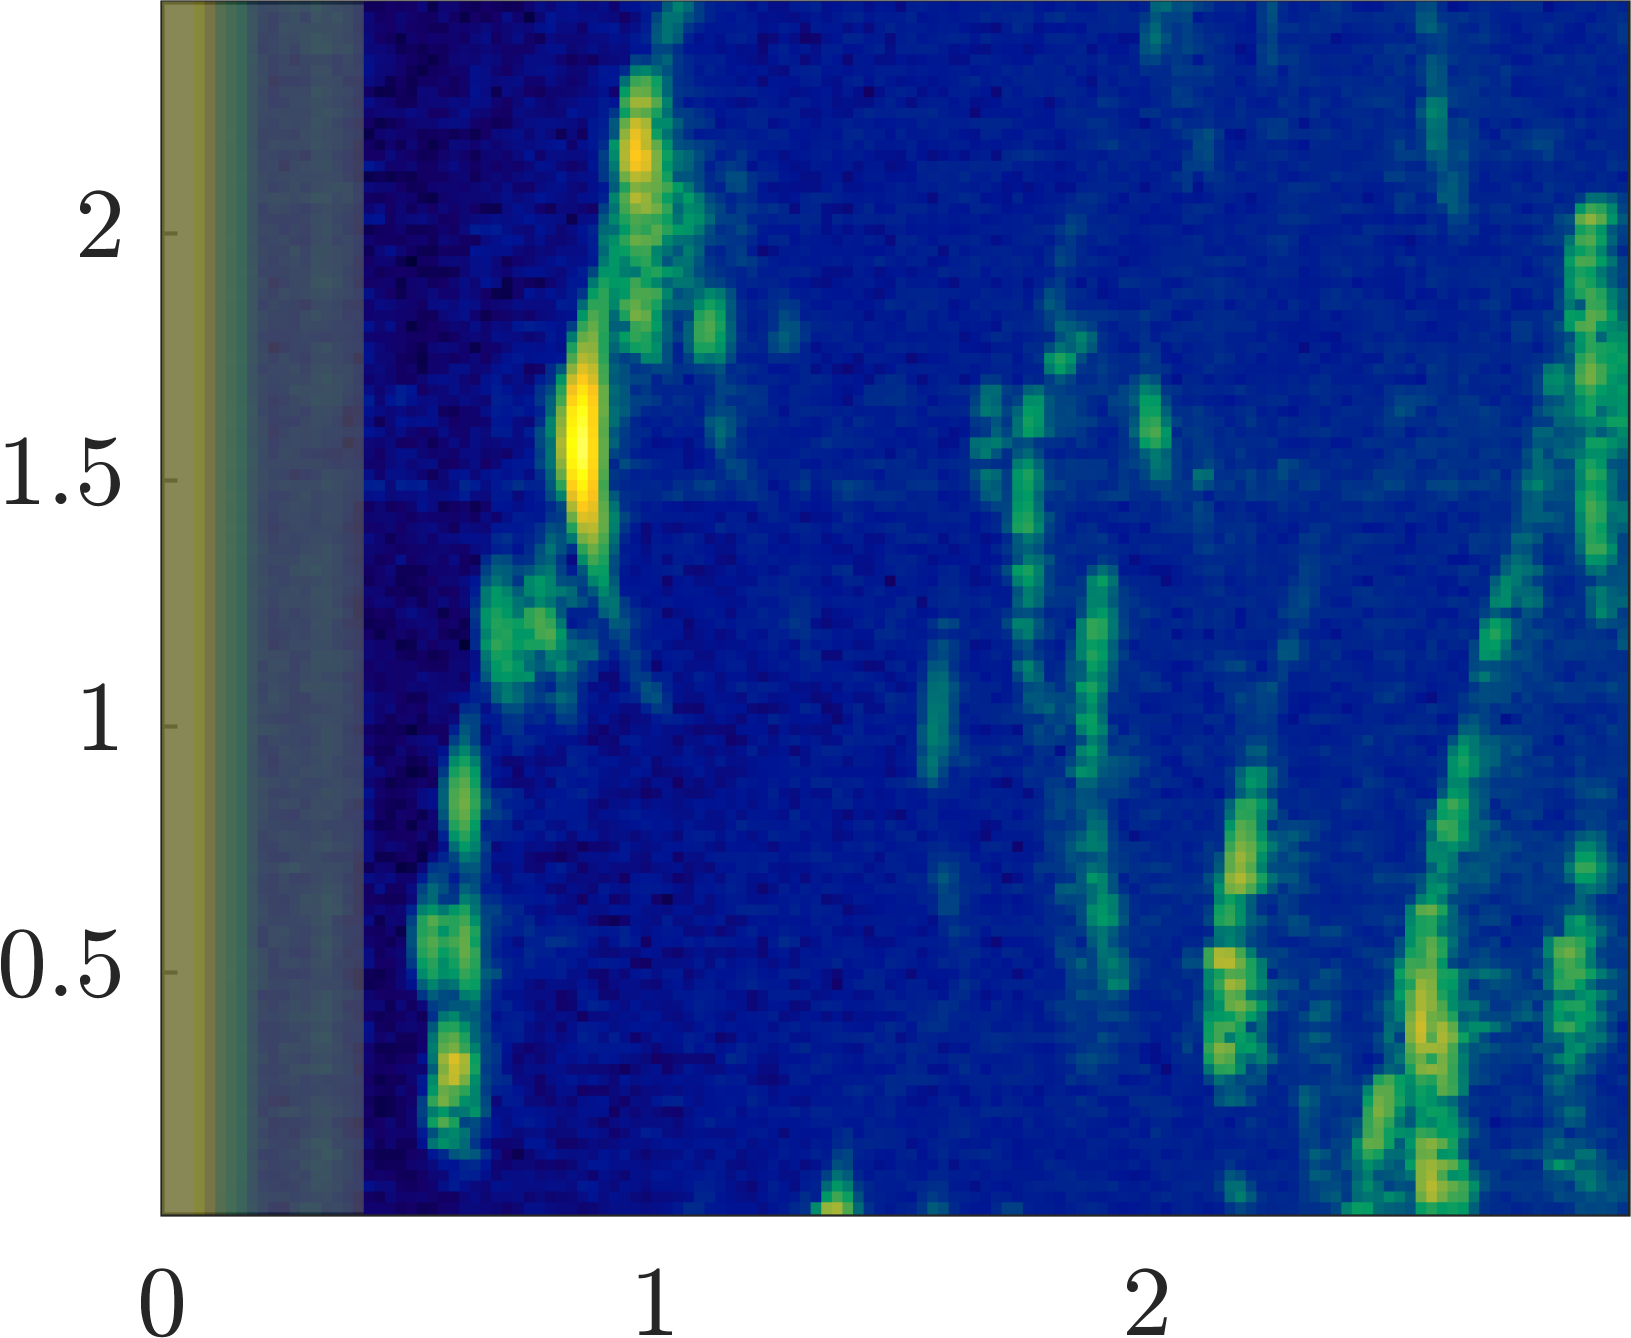
\includegraphics[width=4cm]{gfx/results/attic_input}} & \raisebox{-.5\height}{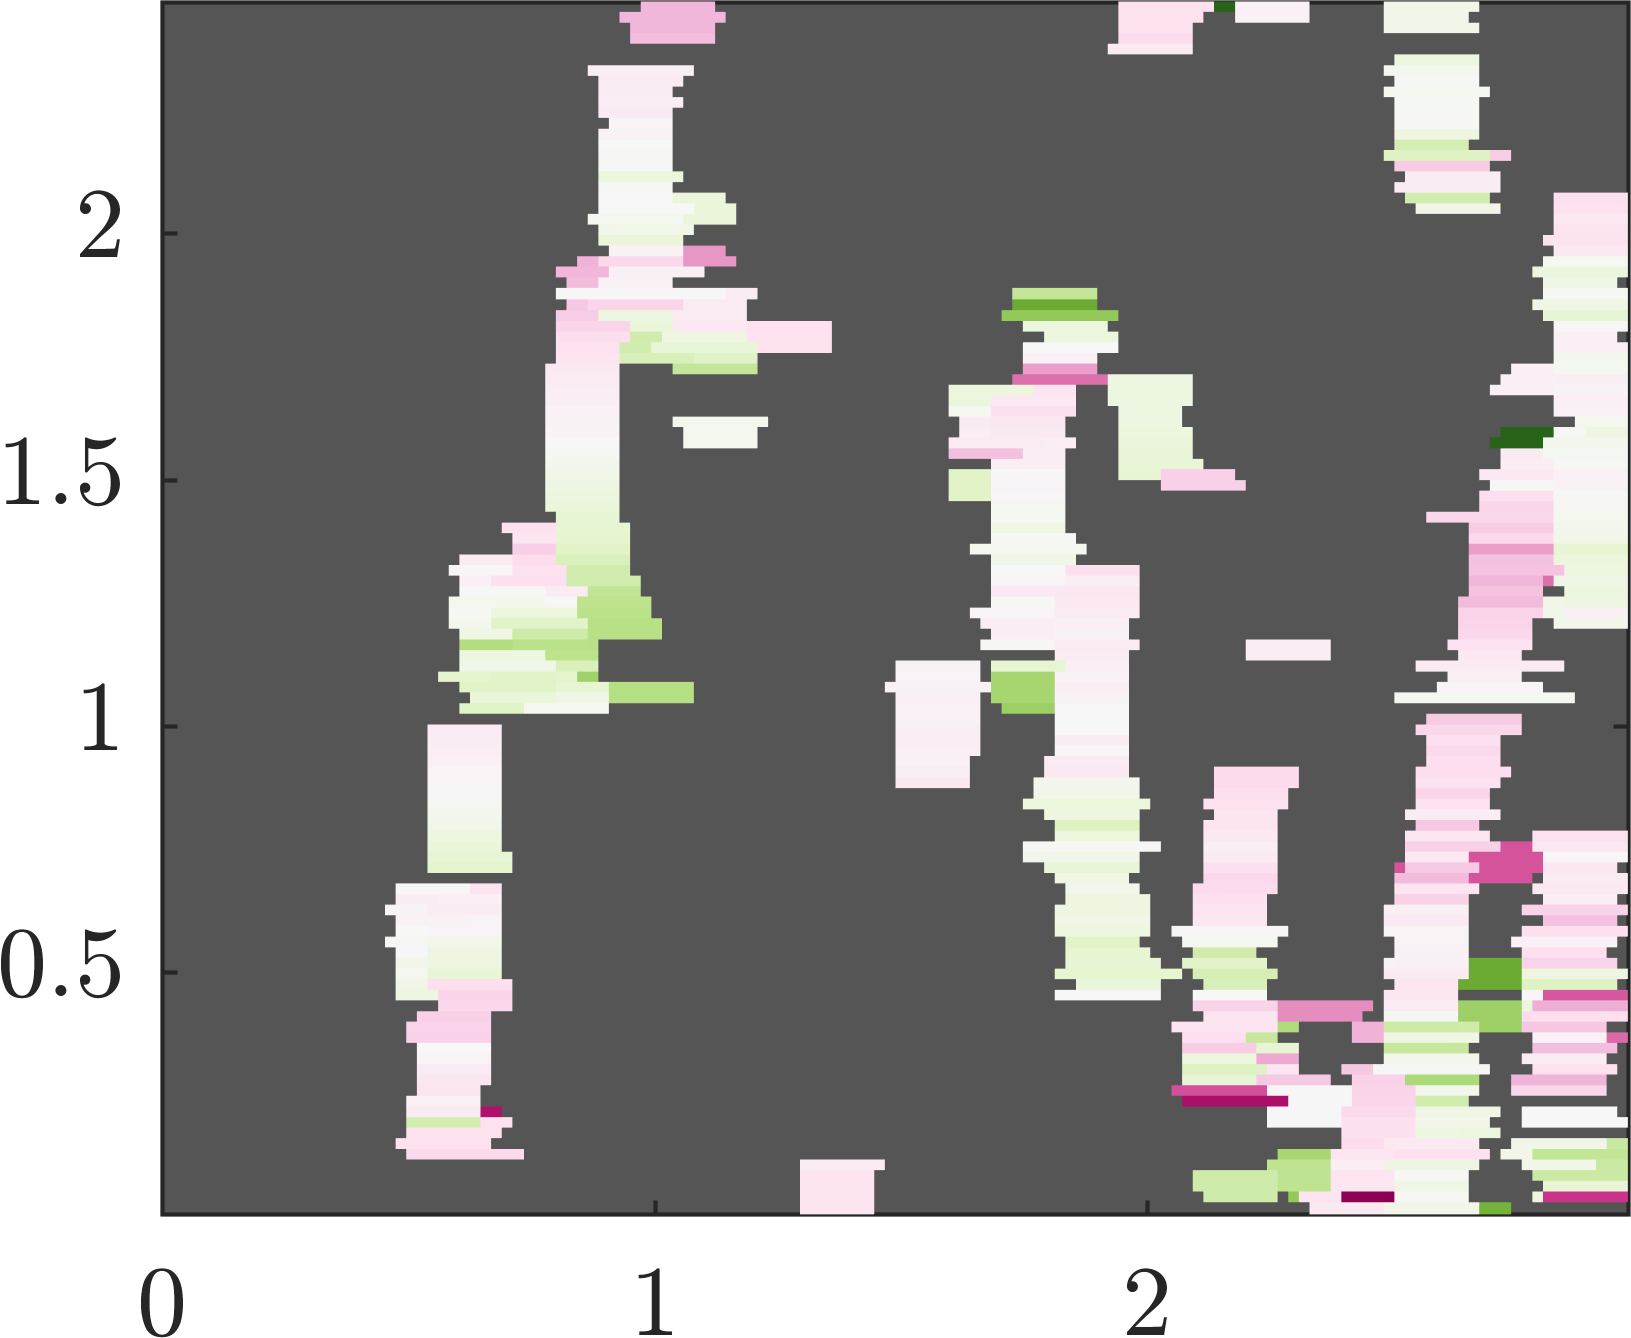
\includegraphics[width=4cm]{gfx/results/attic_doppler}} & \raisebox{-.5\height}{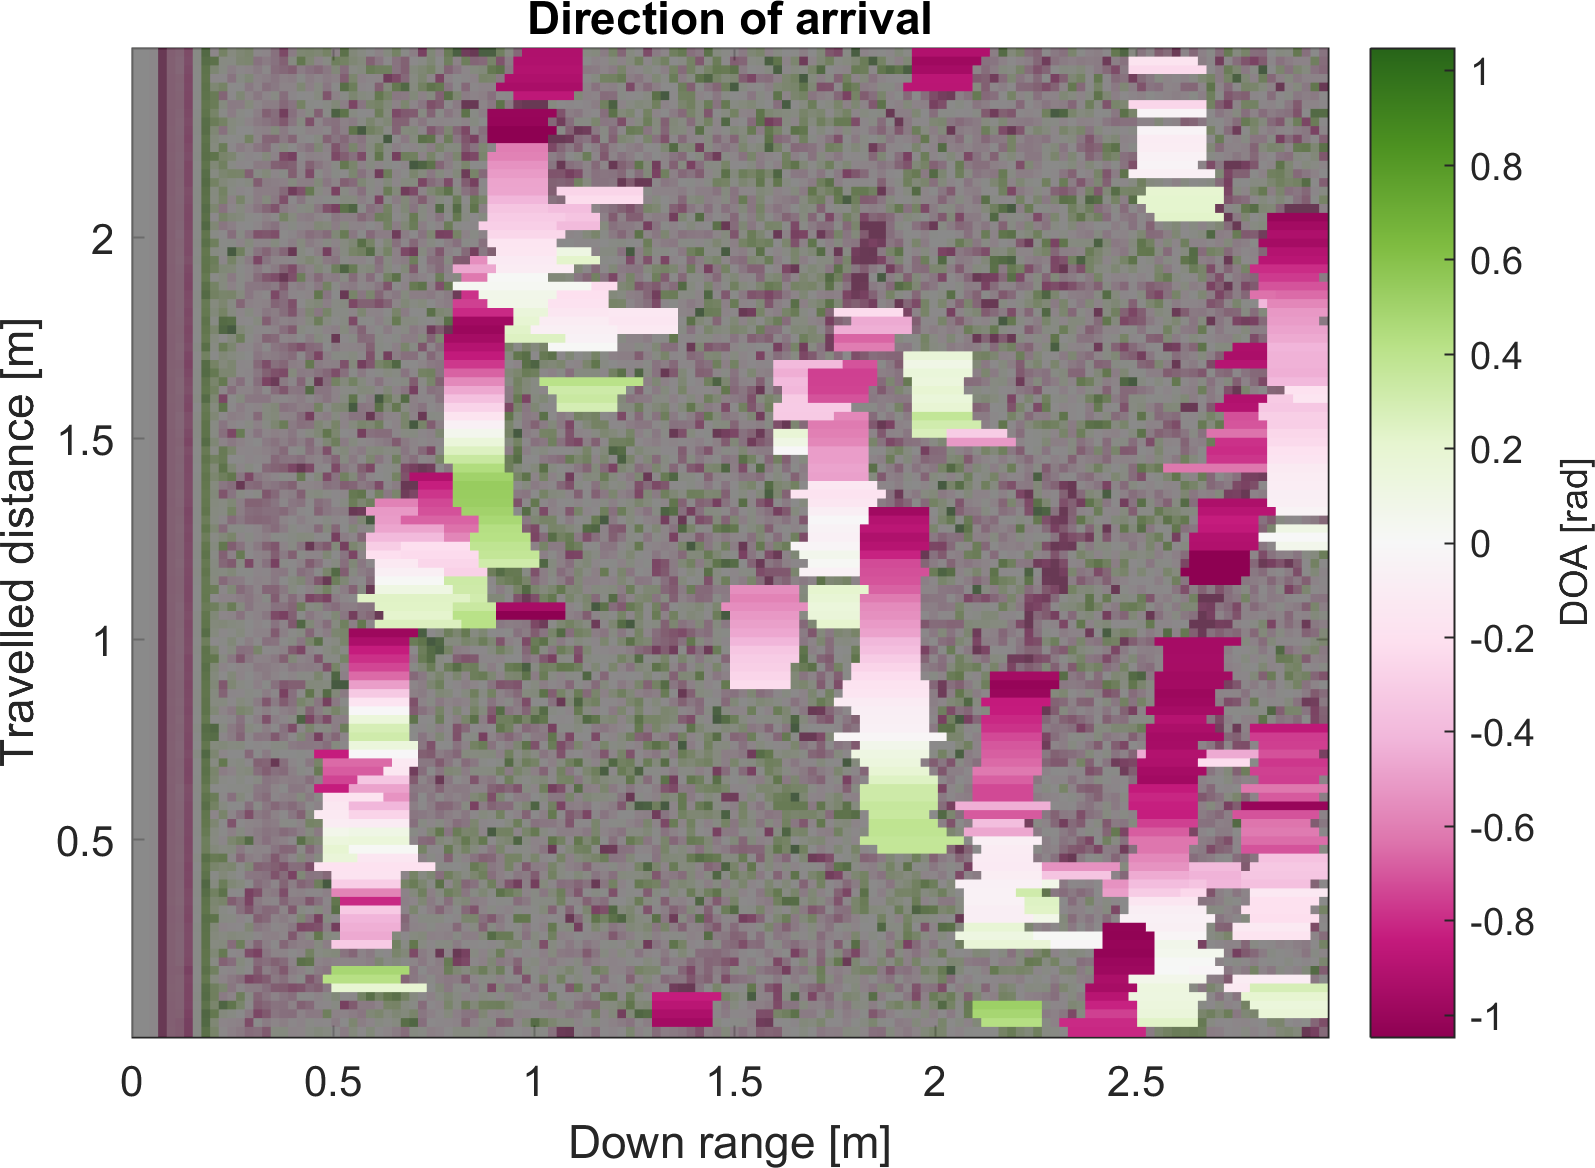
\includegraphics[width=4cm]{gfx/results/attic_doa}} & \raisebox{-.5\height}{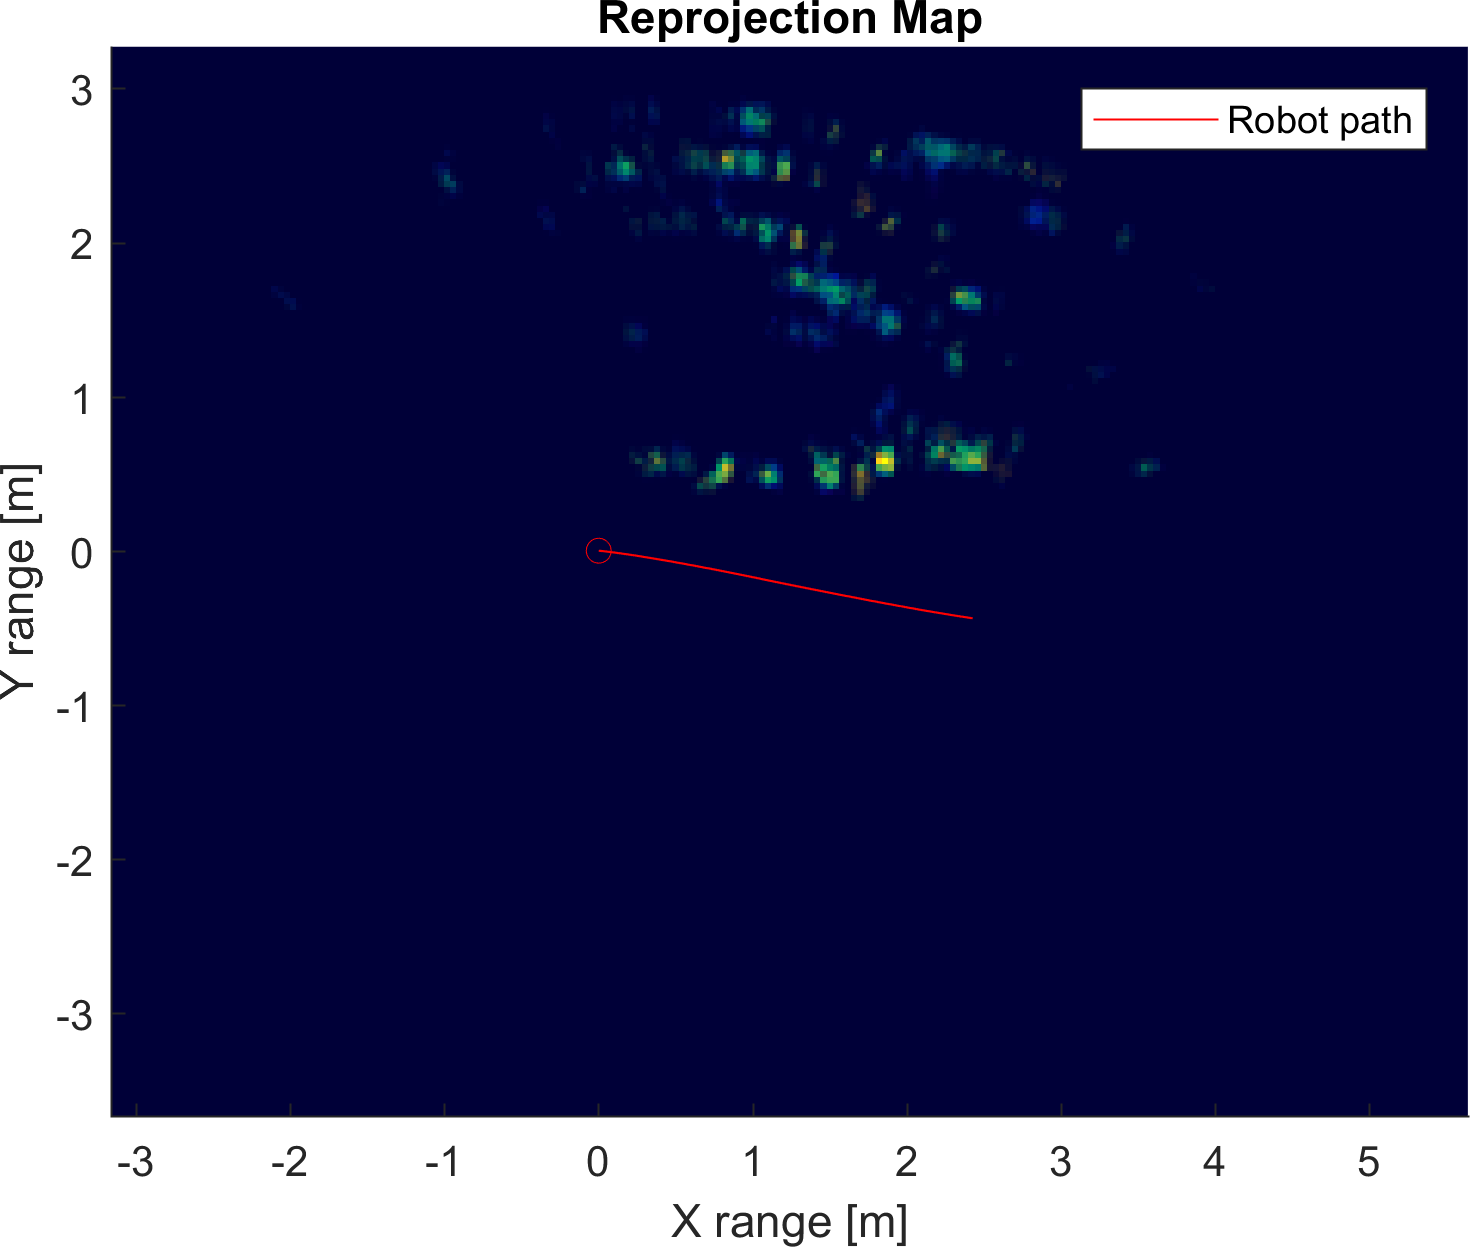
\includegraphics[width=4cm]{gfx/results/attic_reprojection}} & 5ms & H & 90° & \cmark & \xmark & \xmark \\
% Basement & \raisebox{-.5\height}{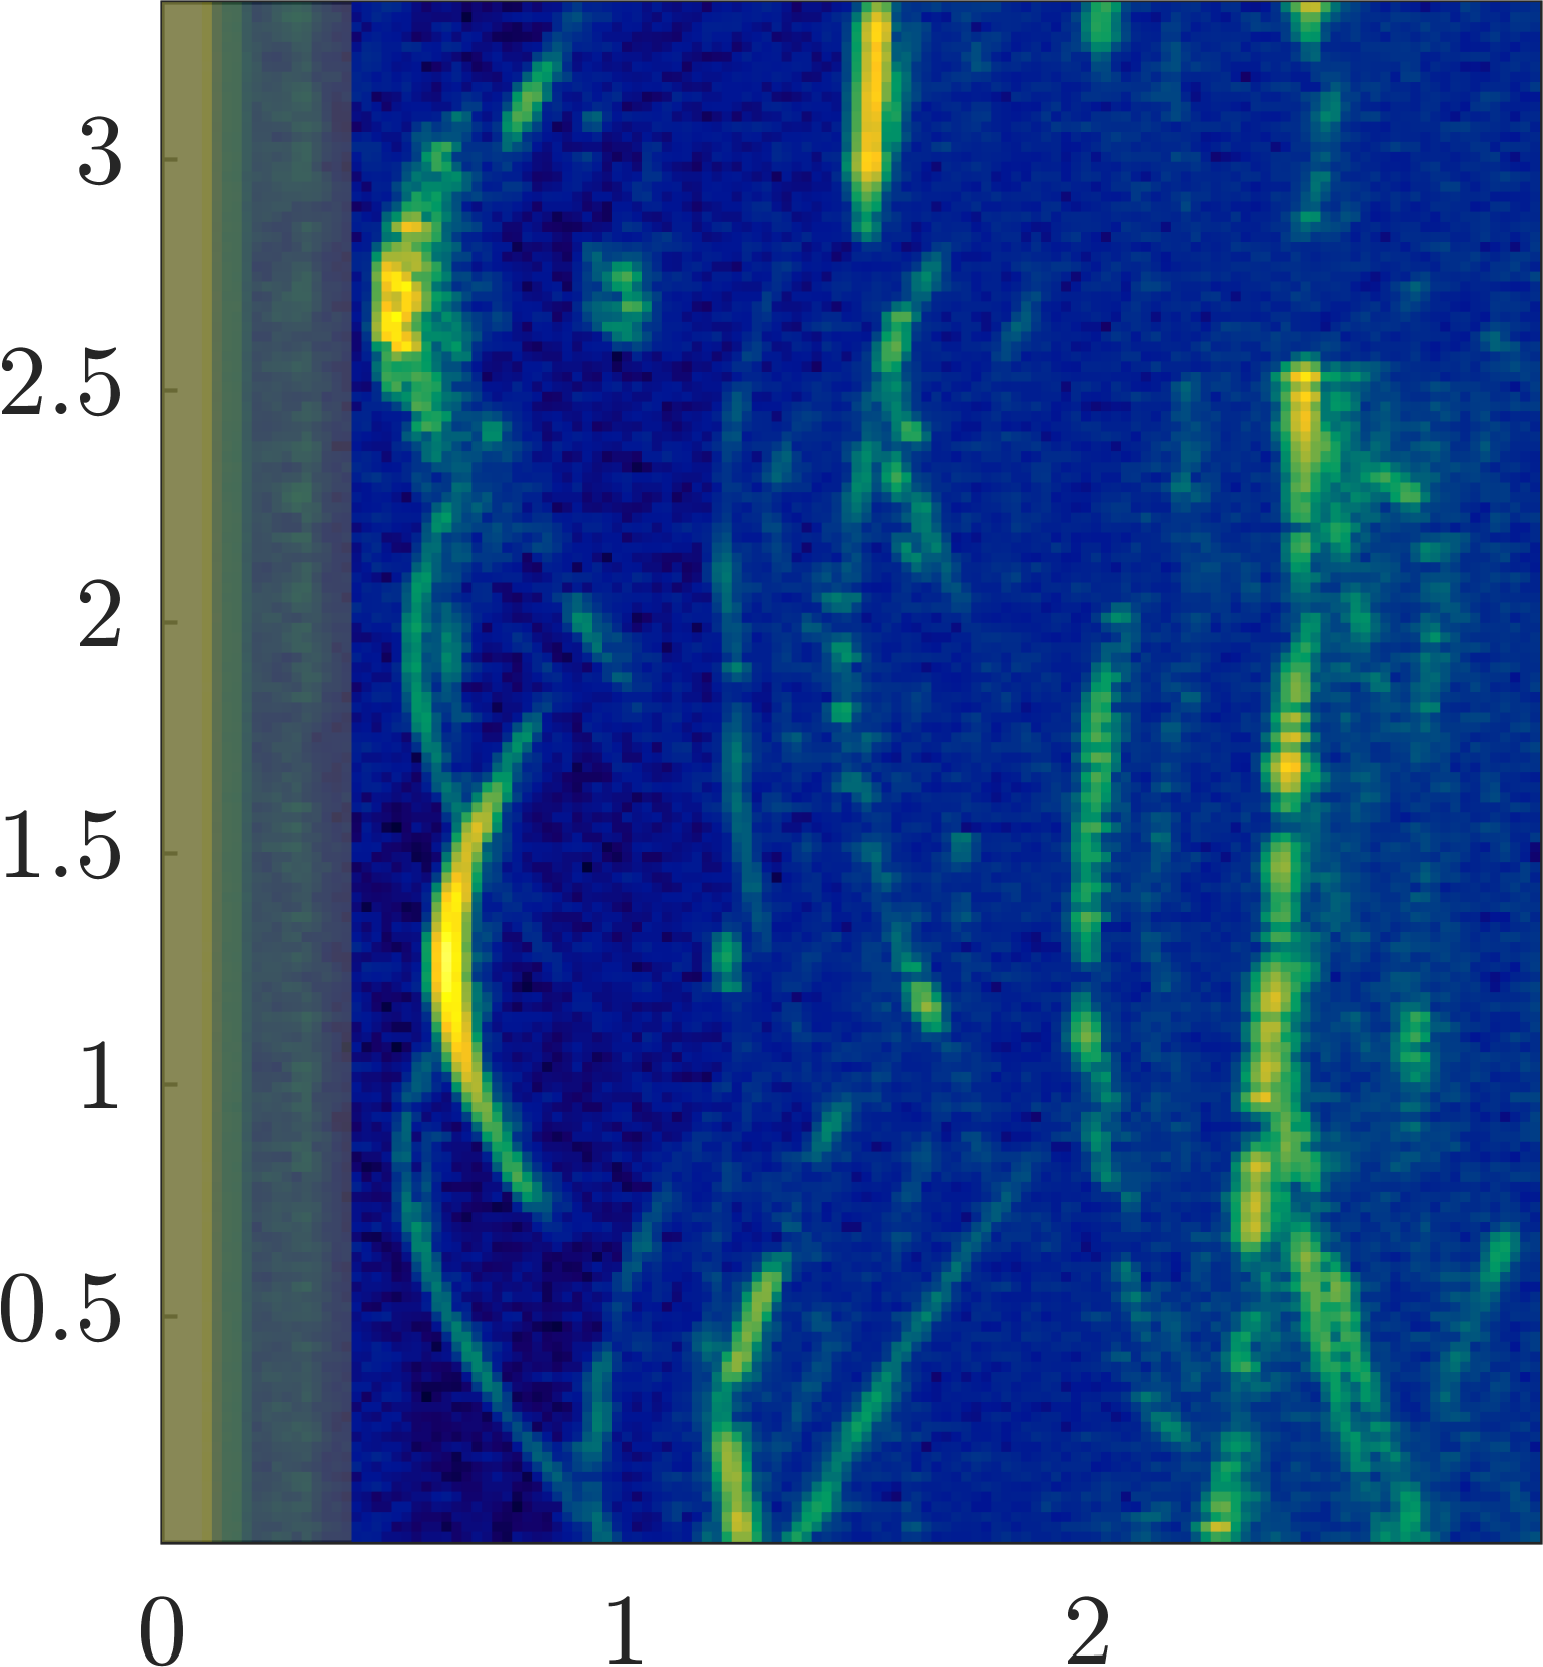
\includegraphics[width=4cm]{gfx/results/basement_input}} & \raisebox{-.5\height}{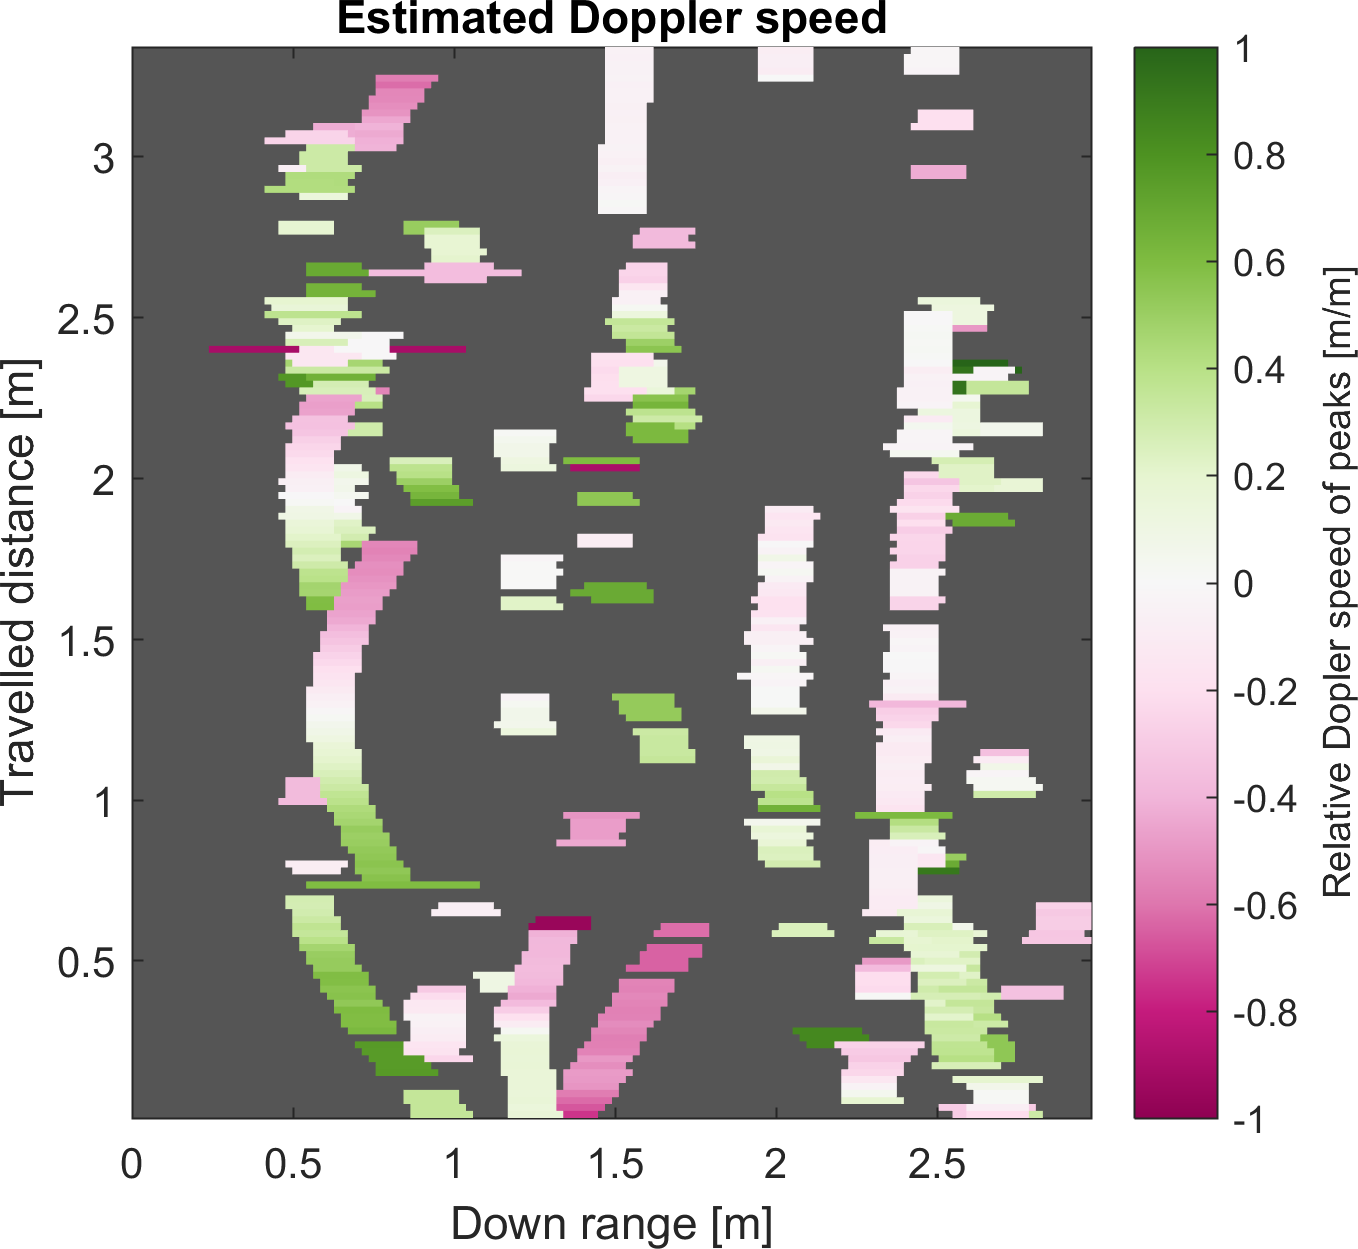
\includegraphics[width=4cm]{gfx/results/basement_doppler}} & \raisebox{-.5\height}{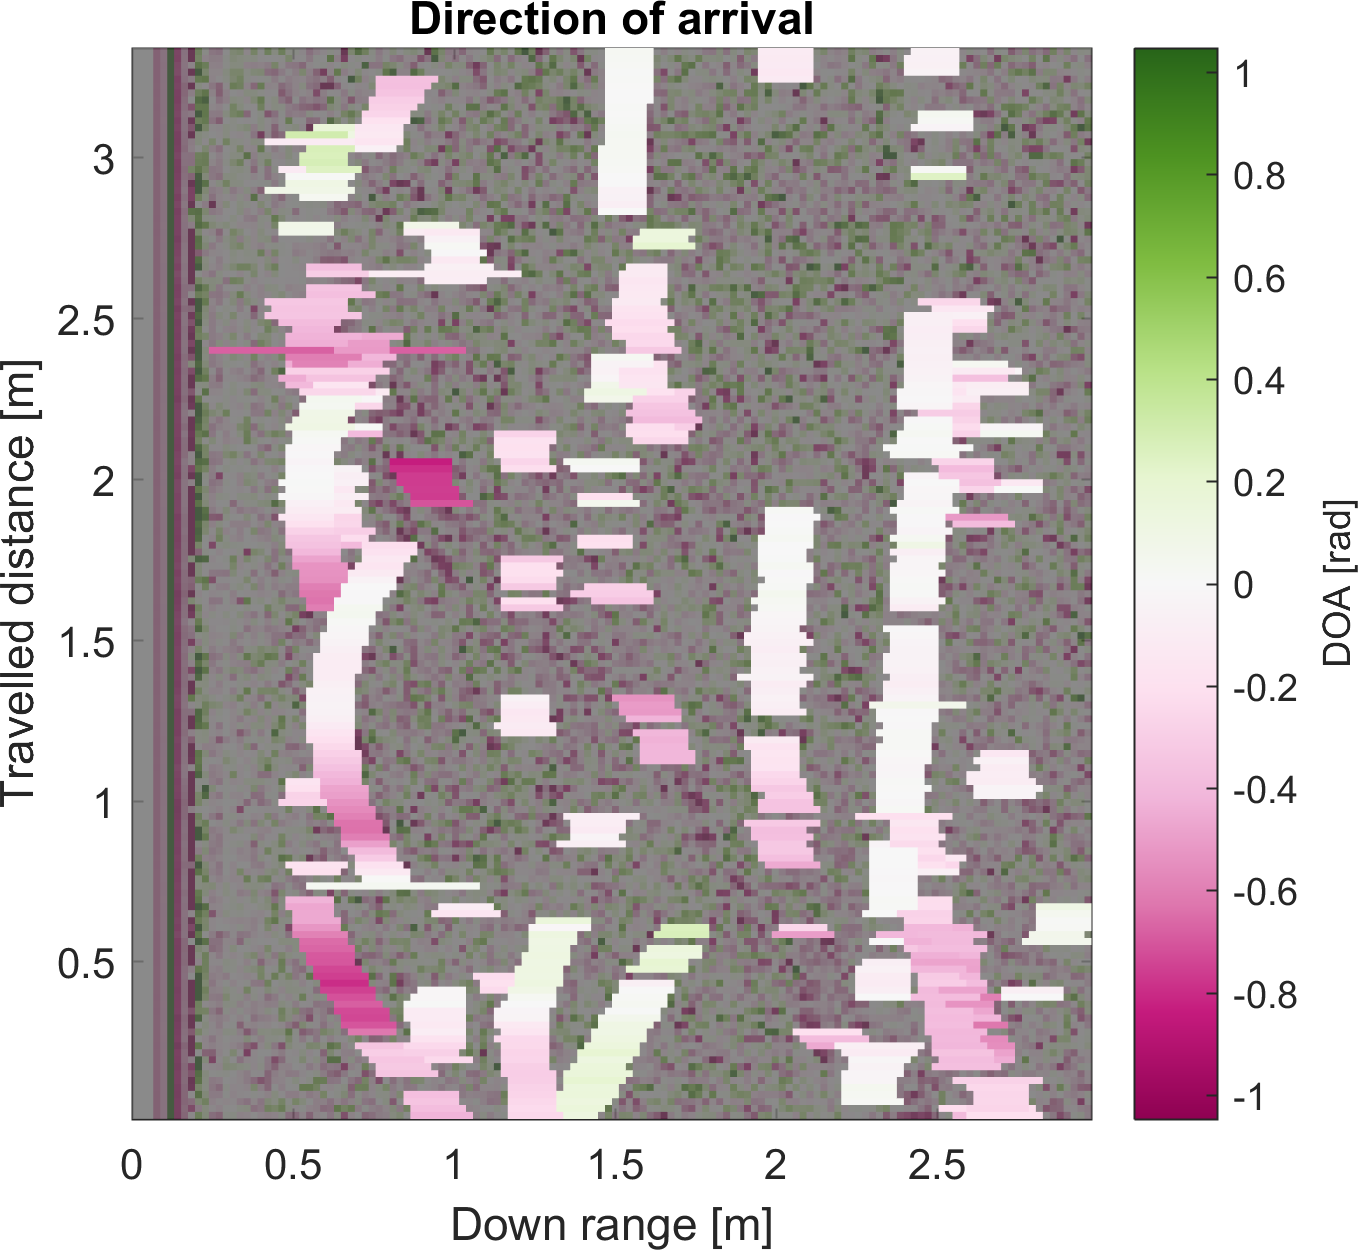
\includegraphics[width=4cm]{gfx/results/basement_doa}} & \raisebox{-.5\height}{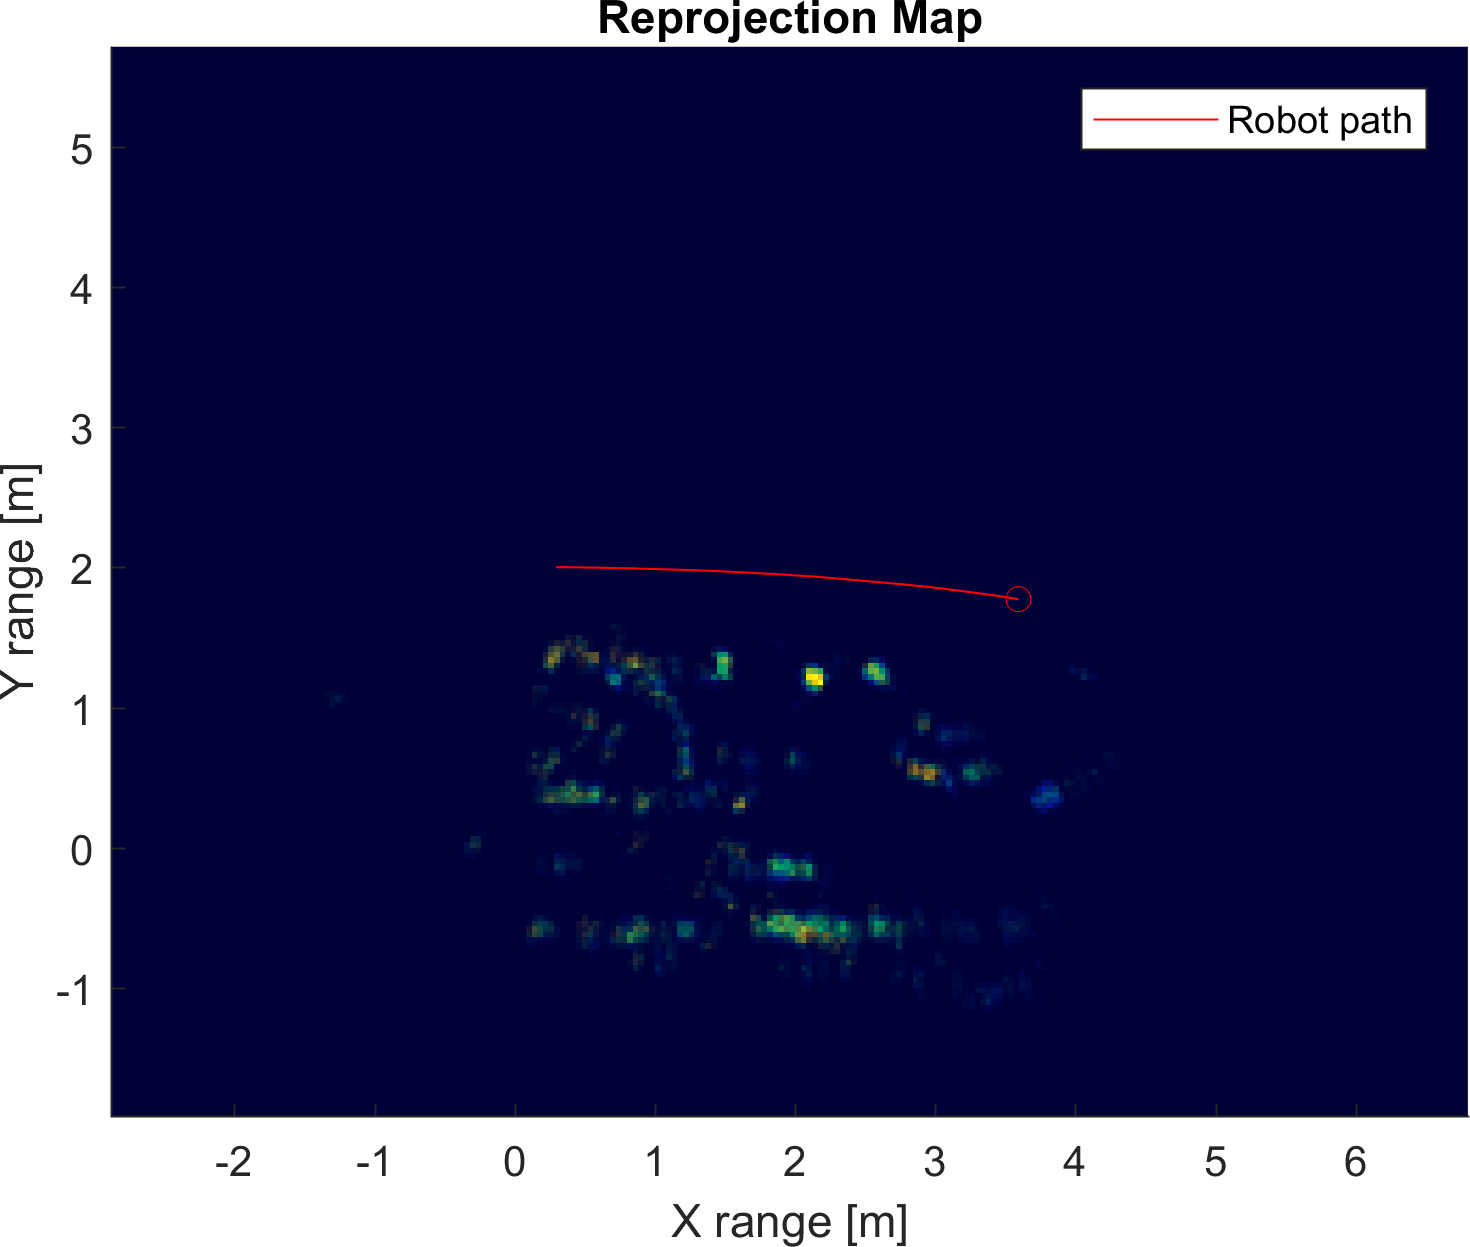
\includegraphics[width=4cm]{gfx/results/basement_reprojection}} & 5ms & H & 90° & \cmark & \xmark & \xmark \\
% Cafeteria                         & \raisebox{-.5\height}{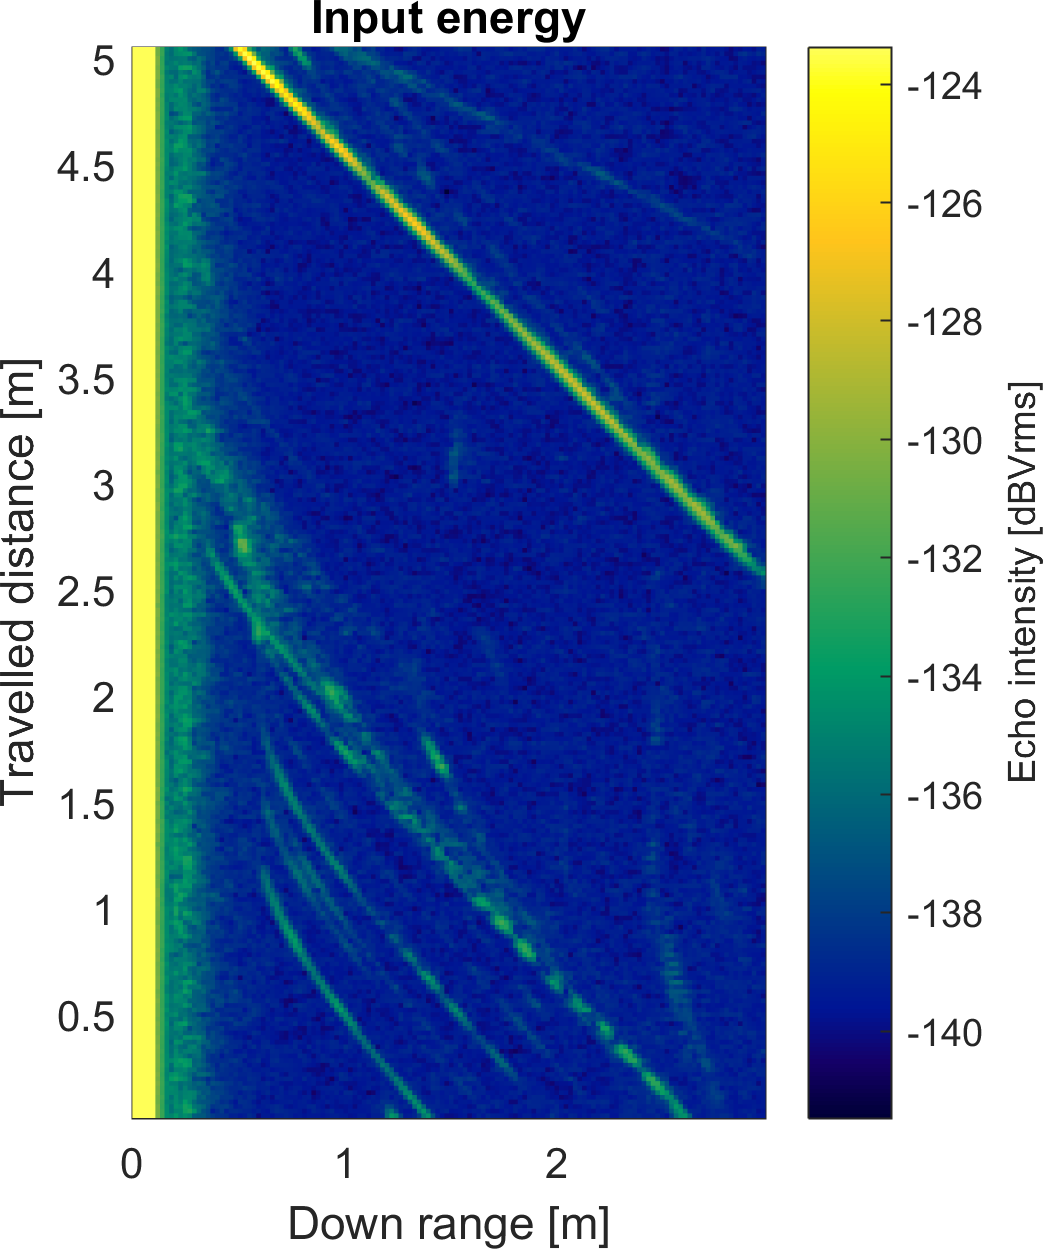
\includegraphics{gfx/results/cafeteria_input}}          & \raisebox{-.5\height}{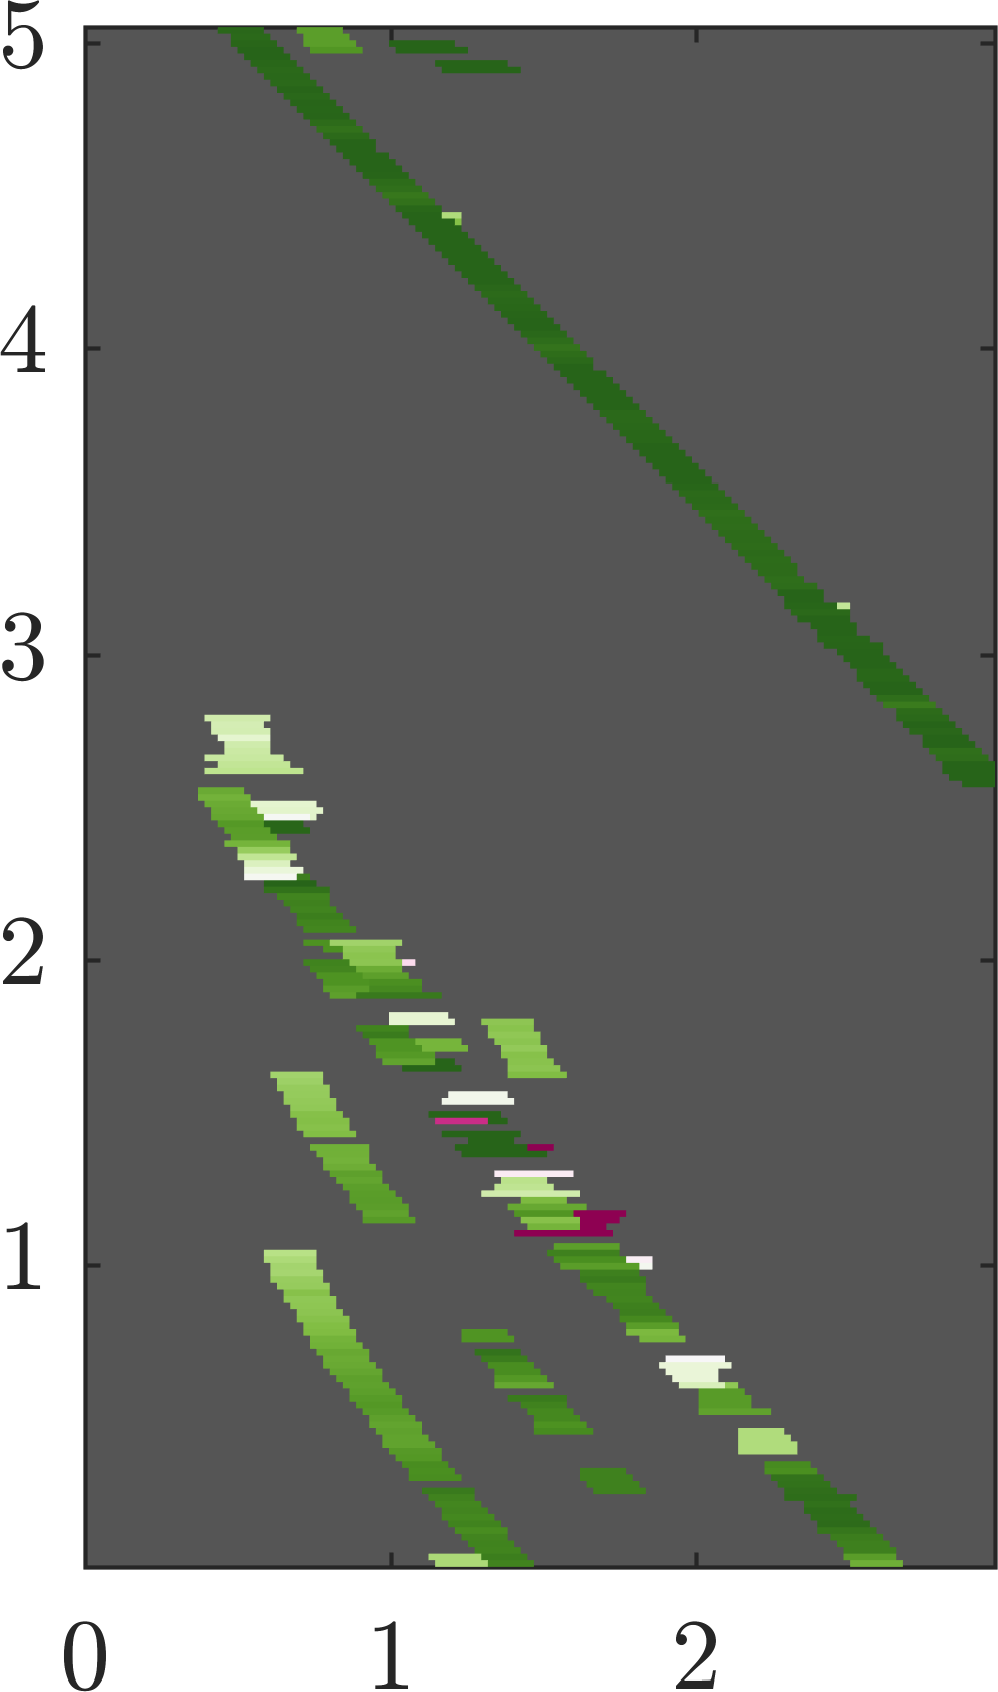
\includegraphics{gfx/results/cafeteria_doppler}}          & \raisebox{-.5\height}{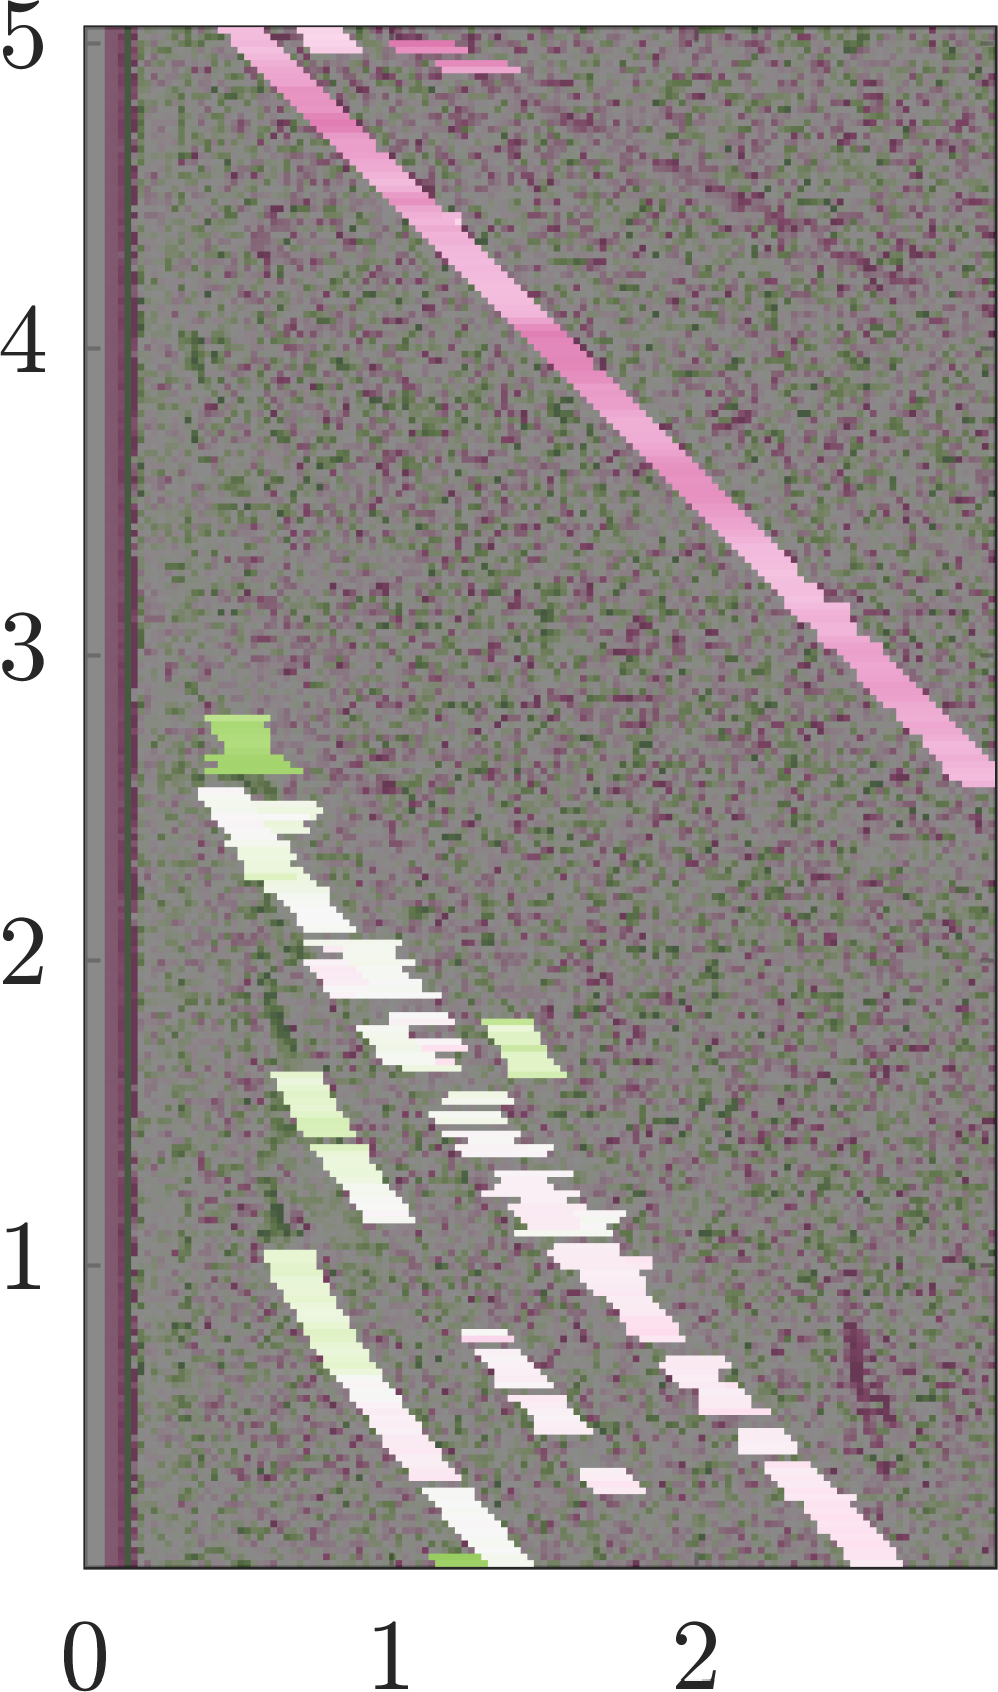
\includegraphics{gfx/results/cafeteria_doa}}          & \raisebox{-.5\height}{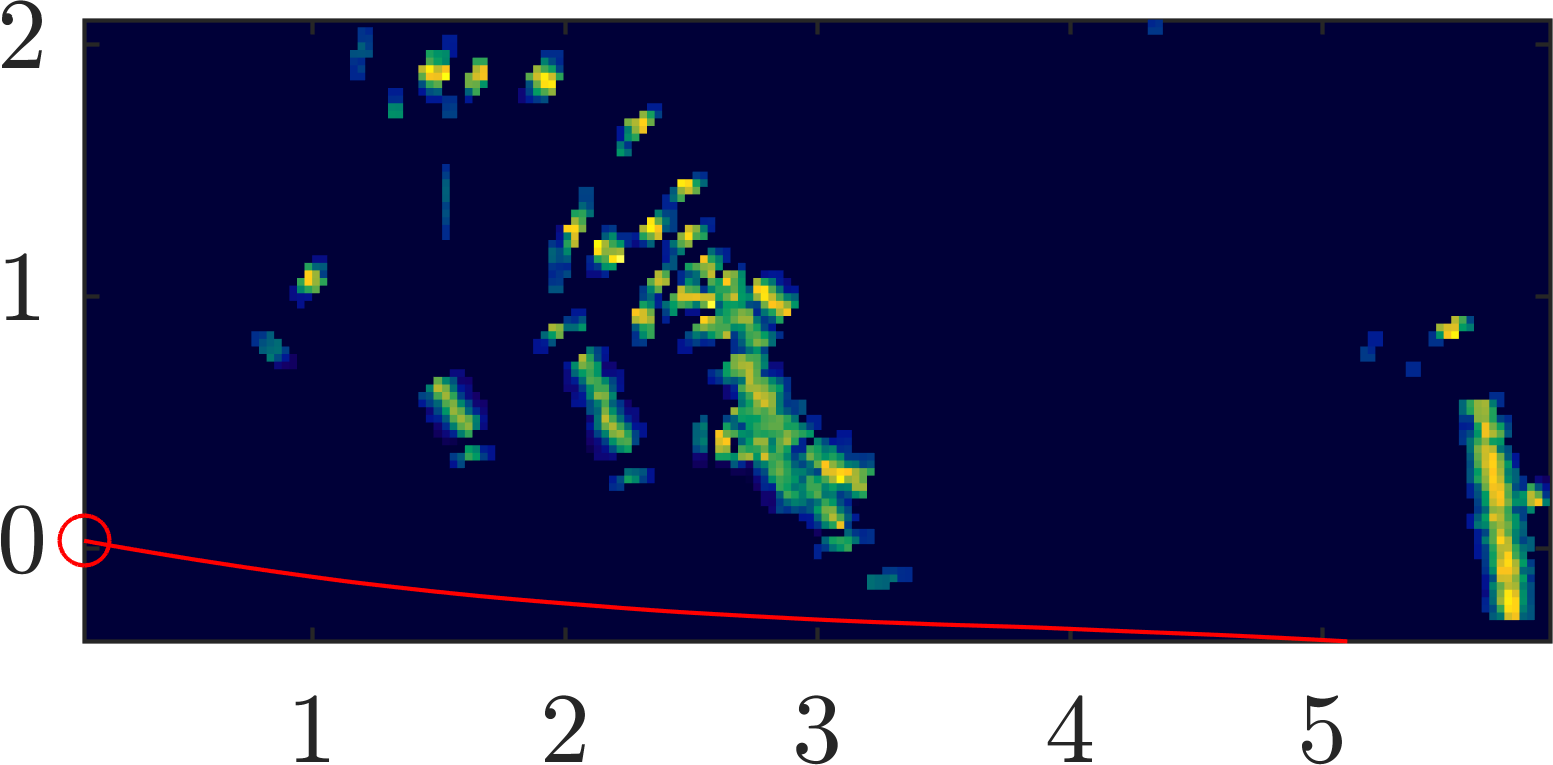
\includegraphics{gfx/results/cafeteria_reprojection}}          & 5ms        & H           & 90°    & \cmark & \xmark & \xmark \\
% Dungeon                           & \raisebox{-.5\height}{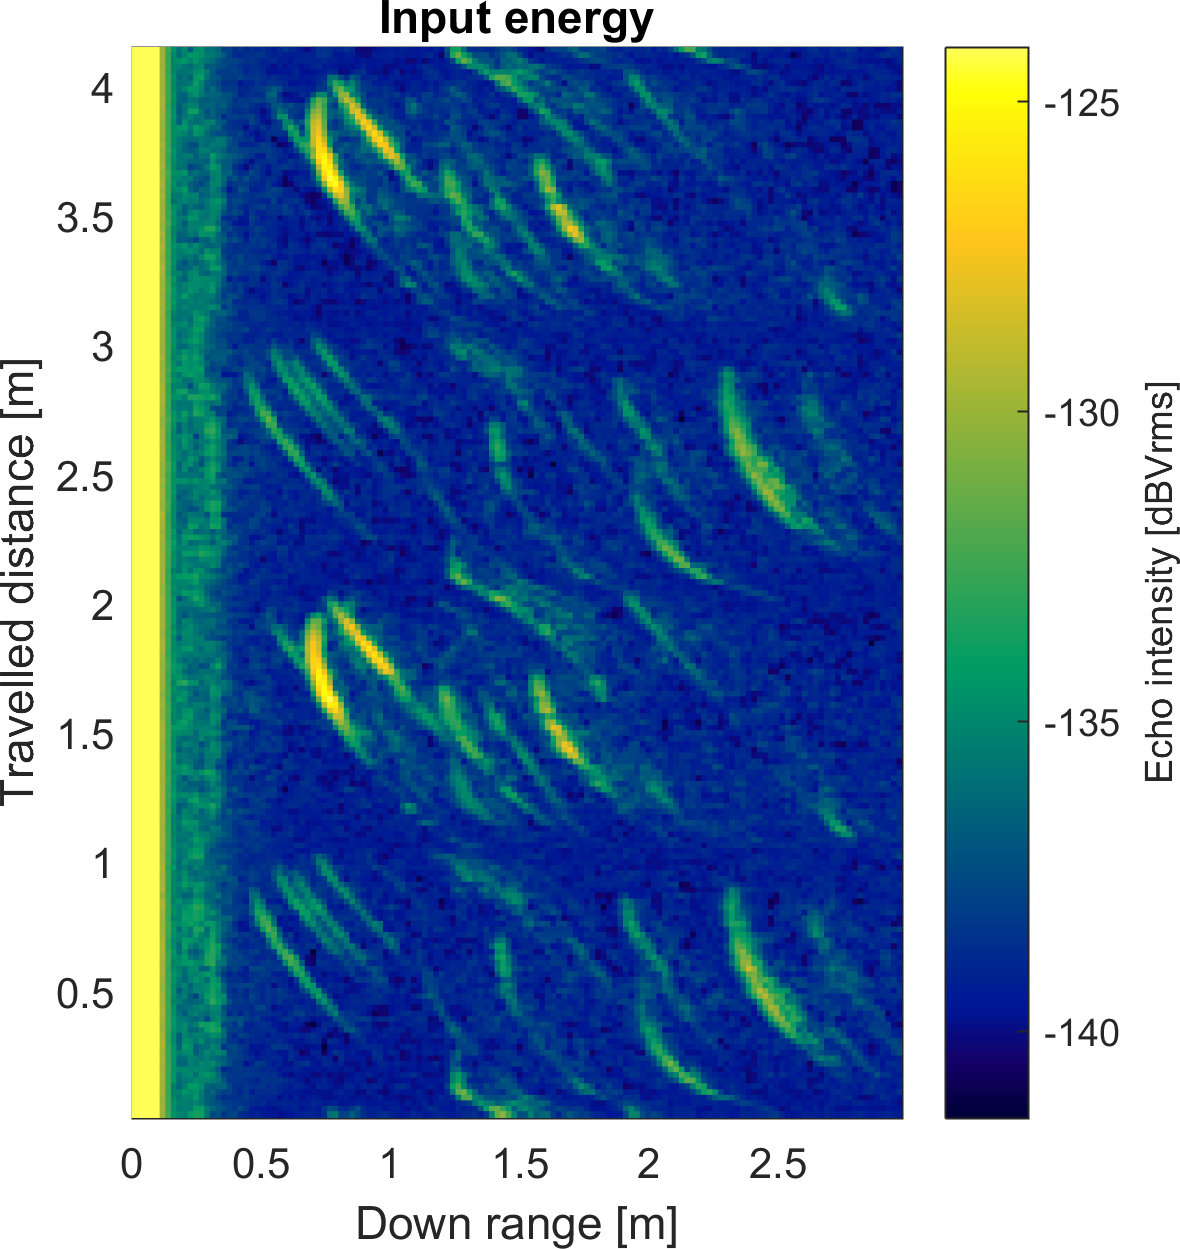
\includegraphics{gfx/results/dungeon_input}}            & \raisebox{-.5\height}{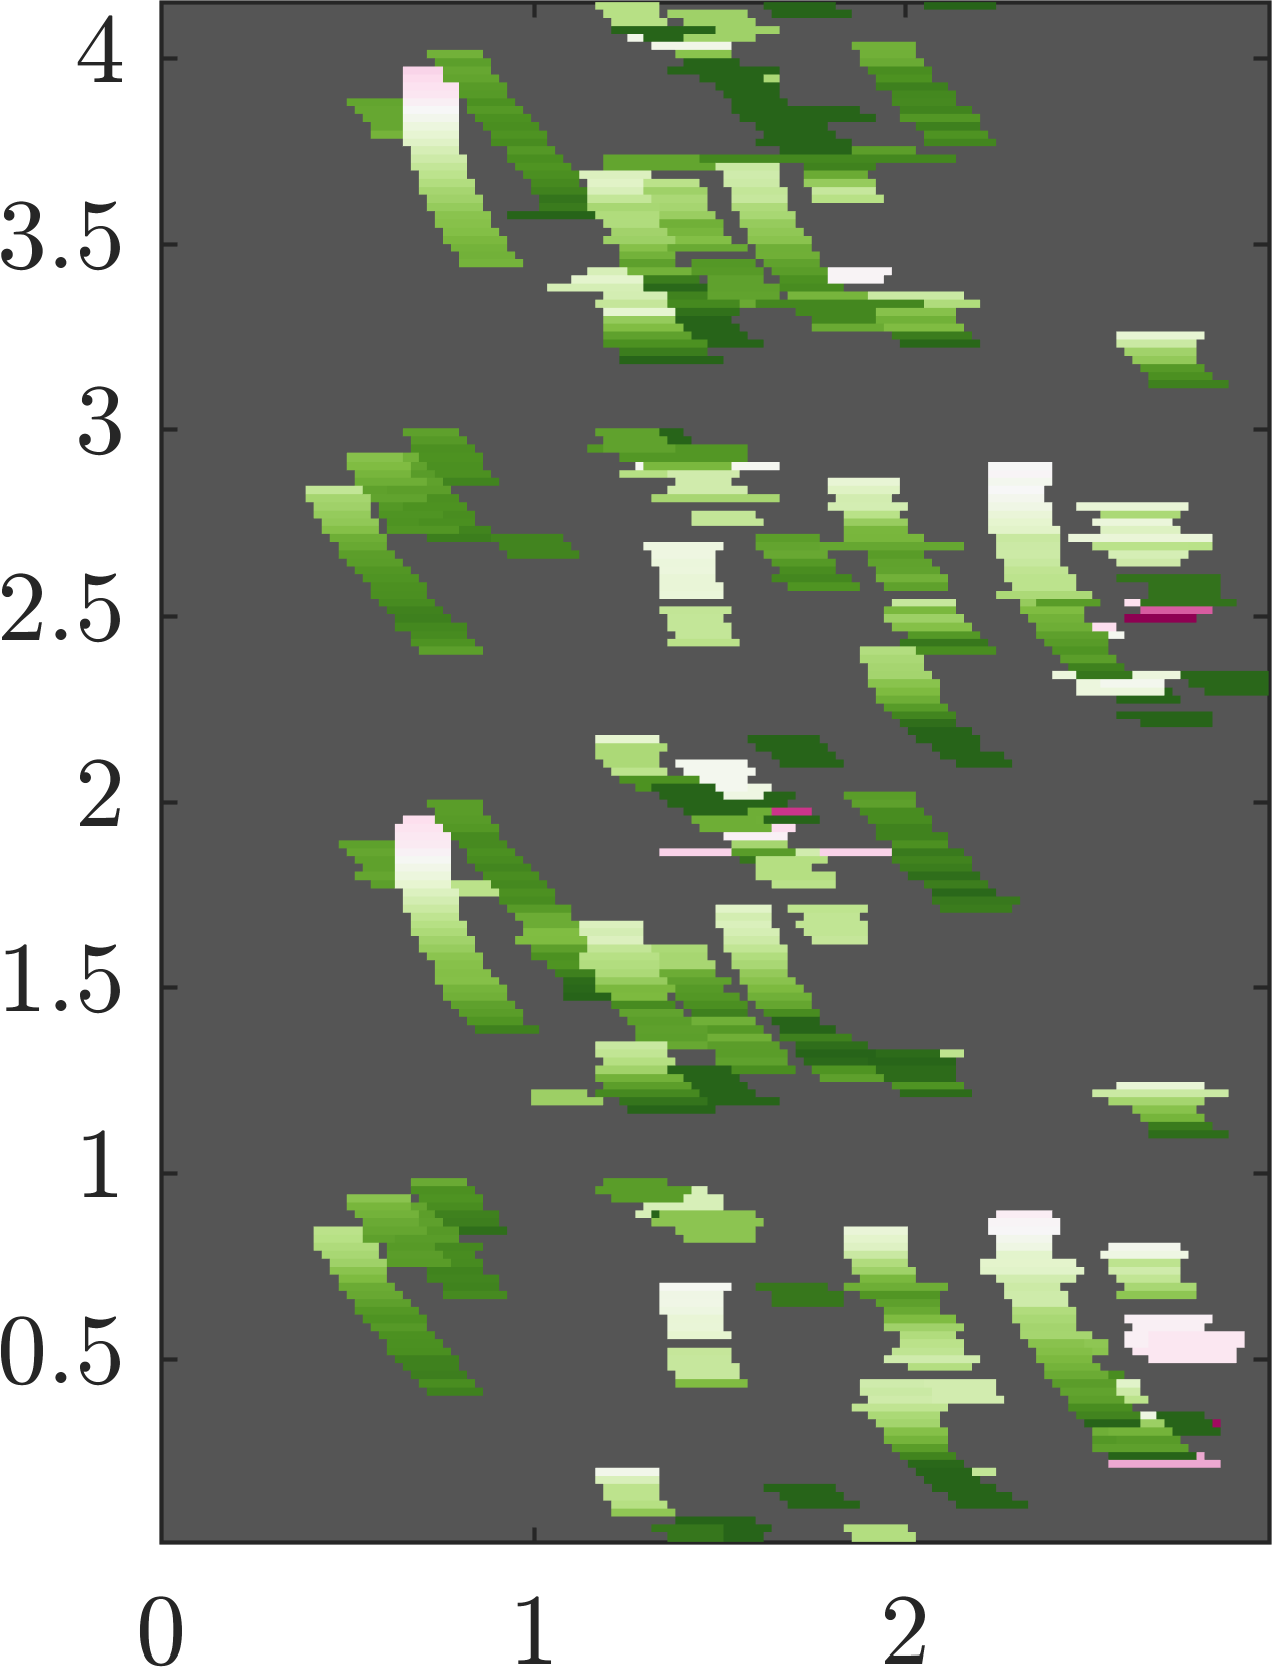
\includegraphics{gfx/results/dungeon_doppler}}            & \raisebox{-.5\height}{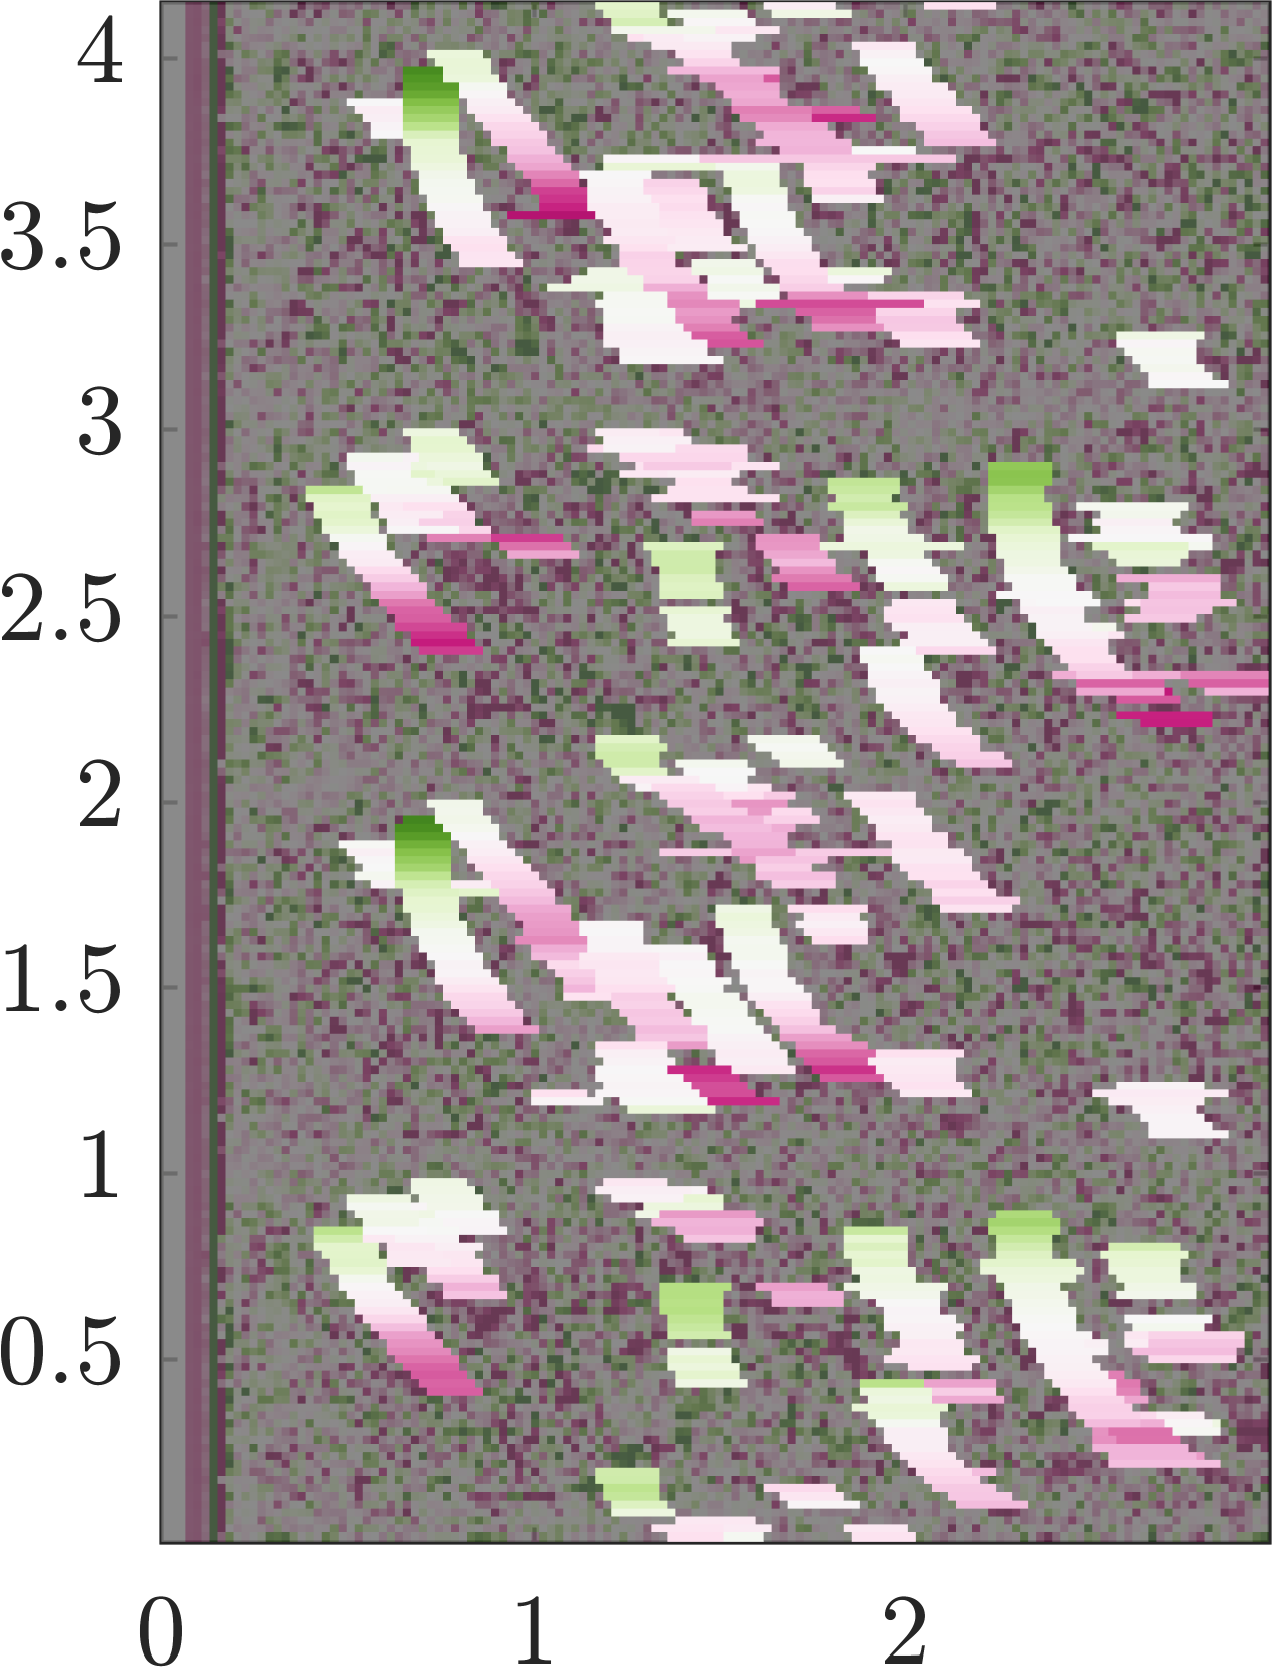
\includegraphics{gfx/results/dungeon_doa}}            & \raisebox{-.5\height}{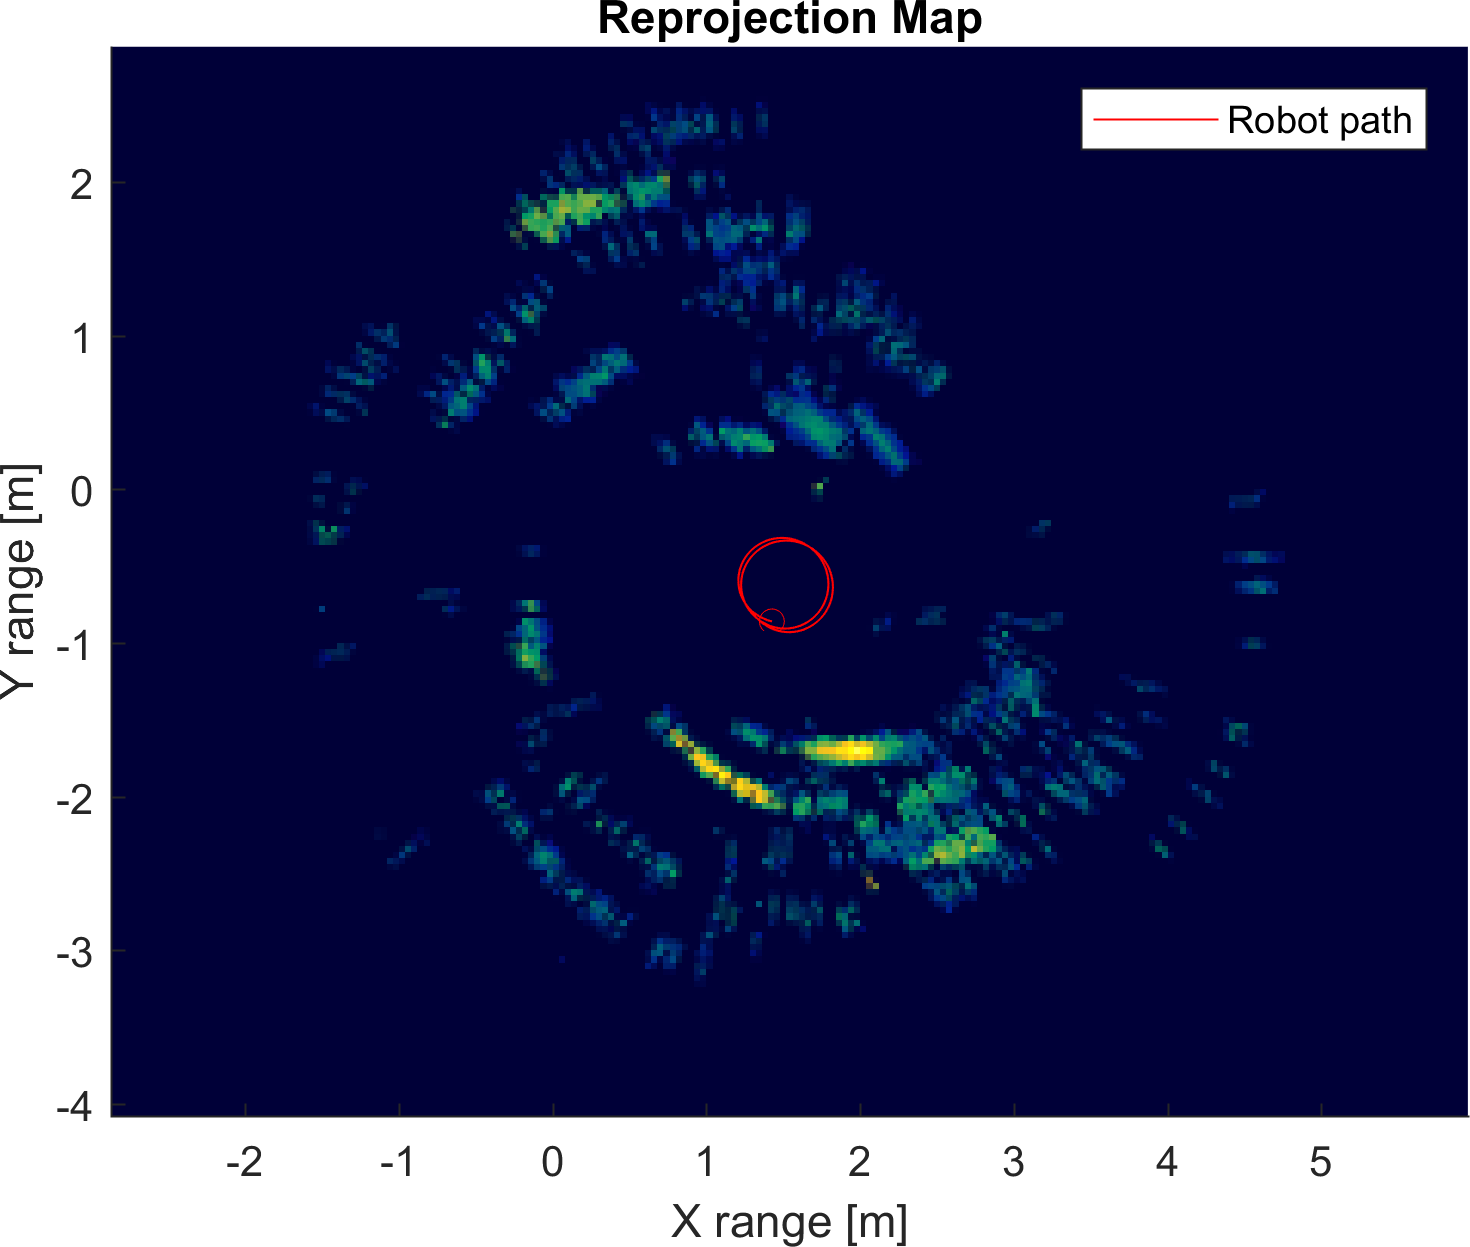
\includegraphics{gfx/results/dungeon_reprojection}}            & 5ms        & V           & 20°    & \cmark & \xmark & \xmark \\
% Entryway                          & \raisebox{-.5\height}{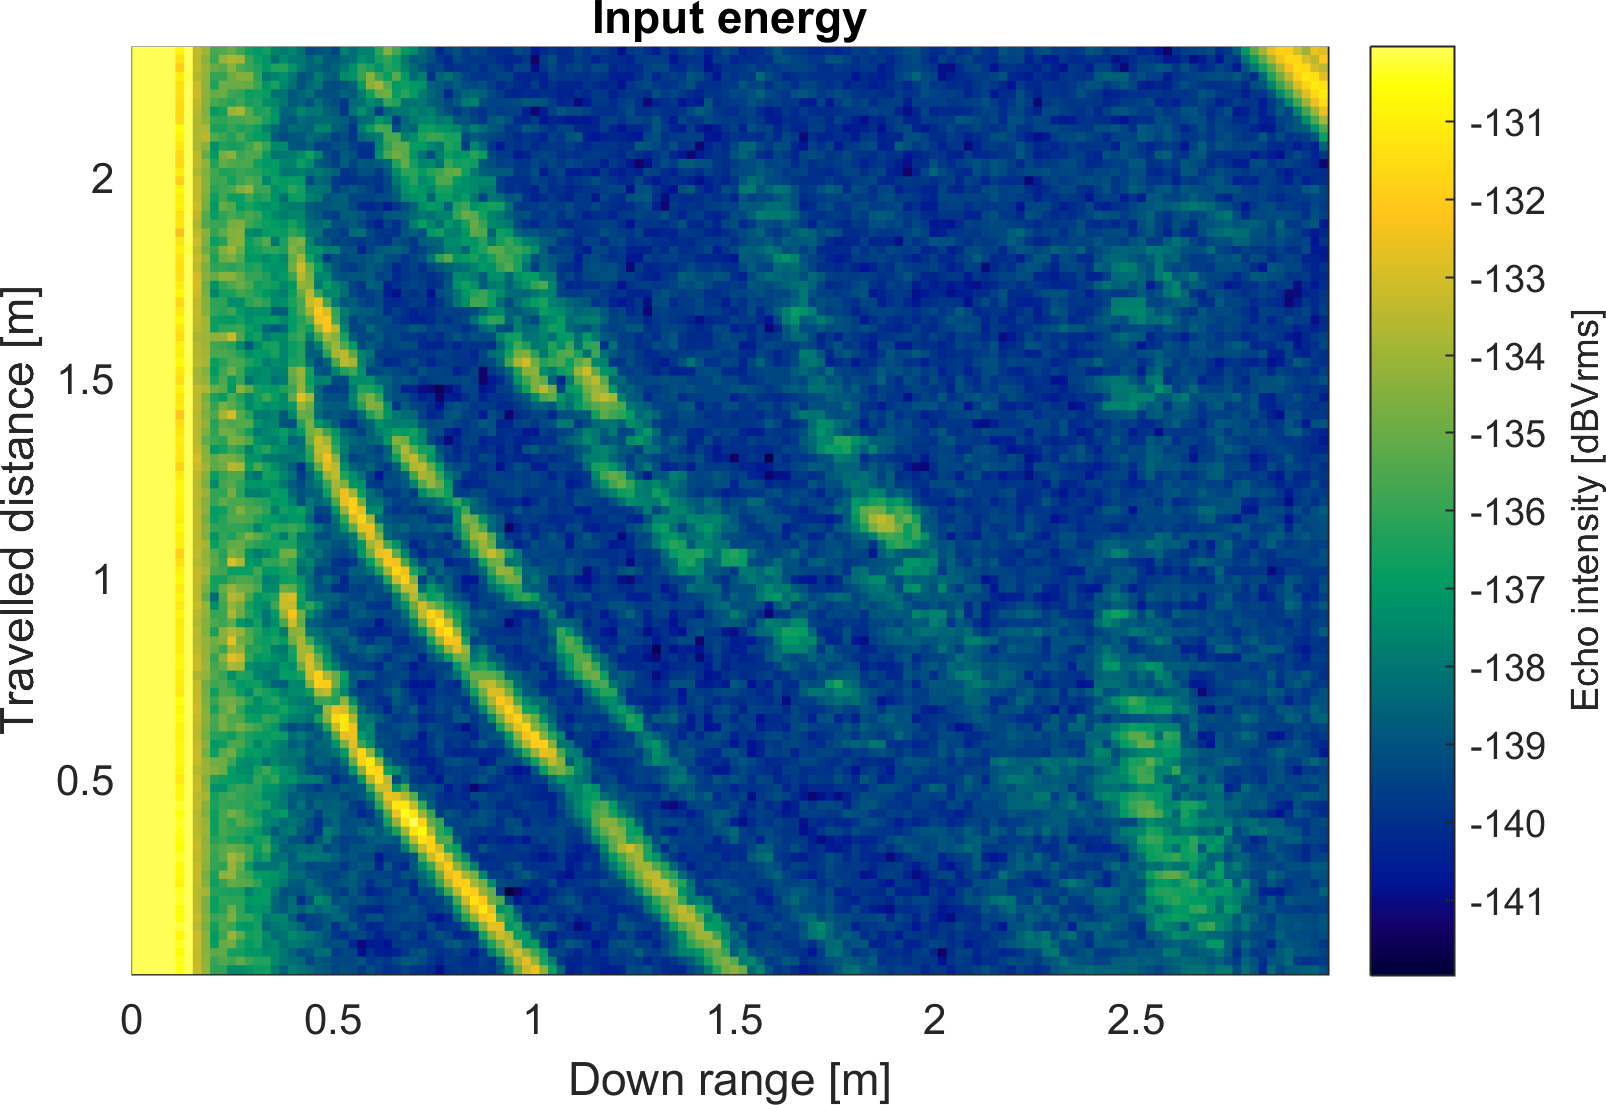
\includegraphics{gfx/results/entryway_input}}           & \raisebox{-.5\height}{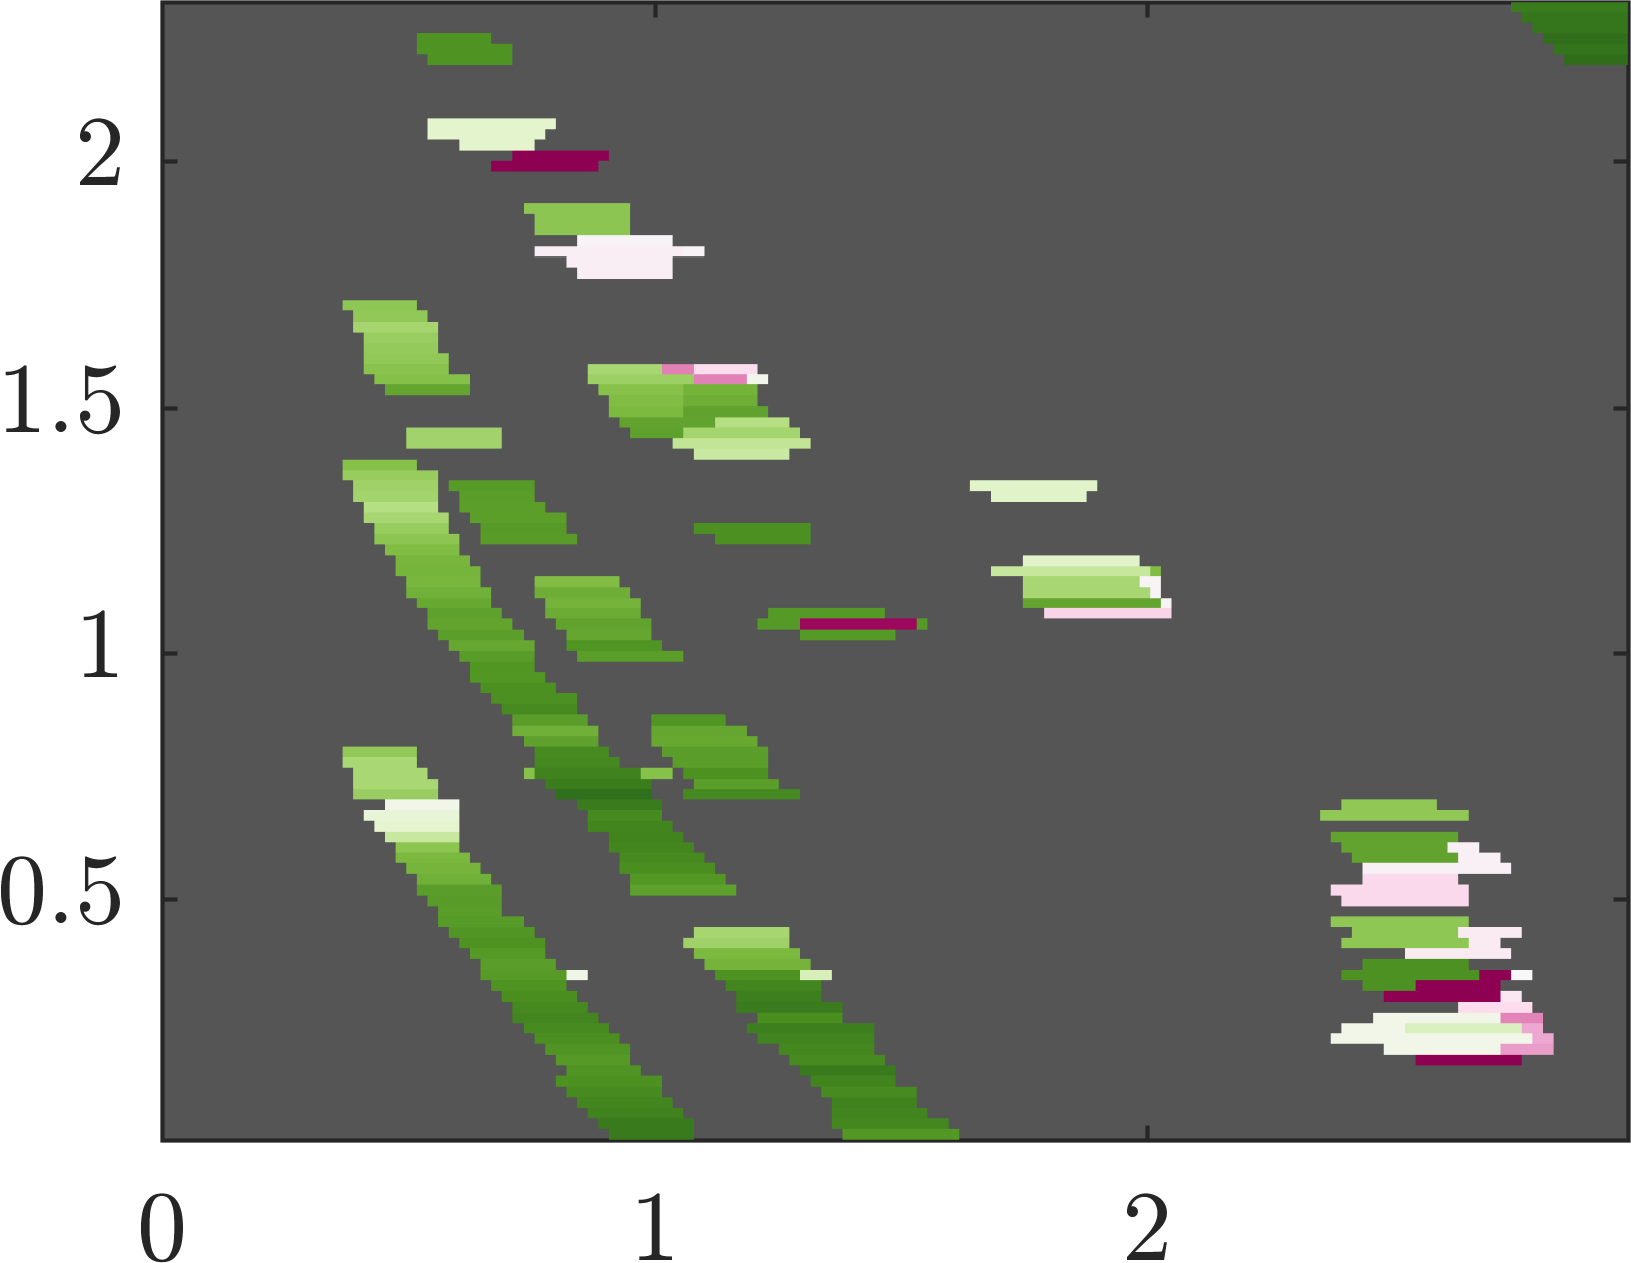
\includegraphics{gfx/results/entryway_doppler}}           & \raisebox{-.5\height}{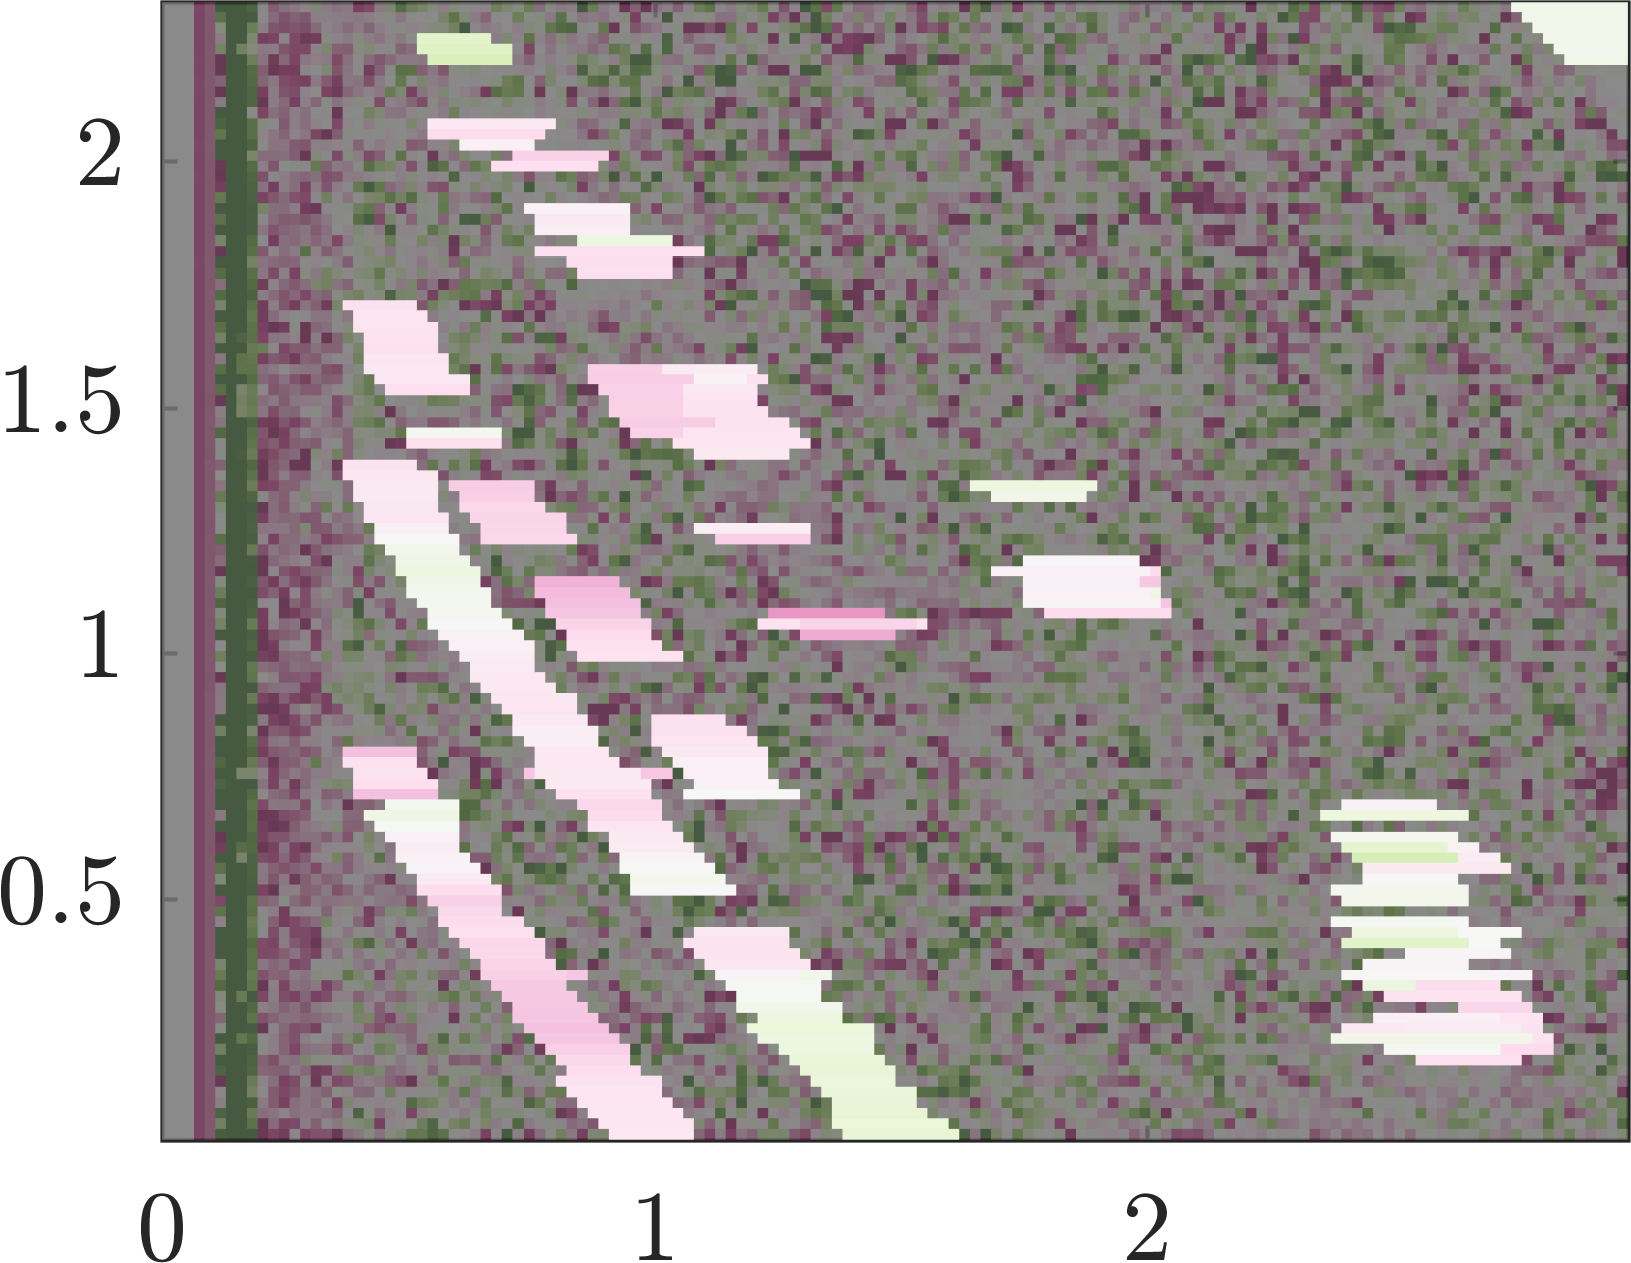
\includegraphics{gfx/results/entryway_doa}}           & \raisebox{-.5\height}{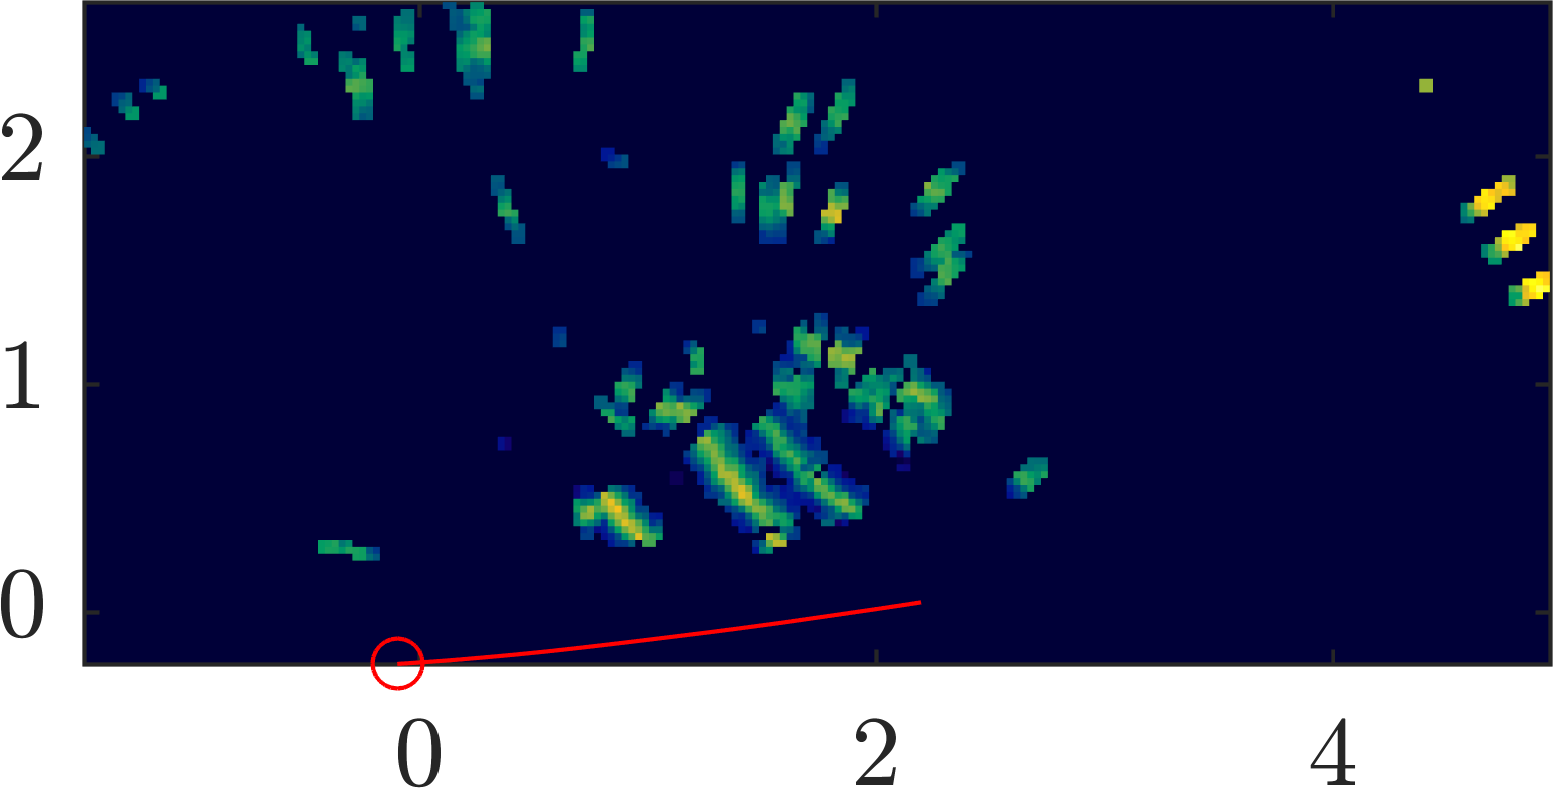
\includegraphics{gfx/results/entryway_reprojection}}           & 5ms        & V           & 20°    & \cmark & \xmark & \xmark \\
% Fallout shelter                   & \raisebox{-.5\height}{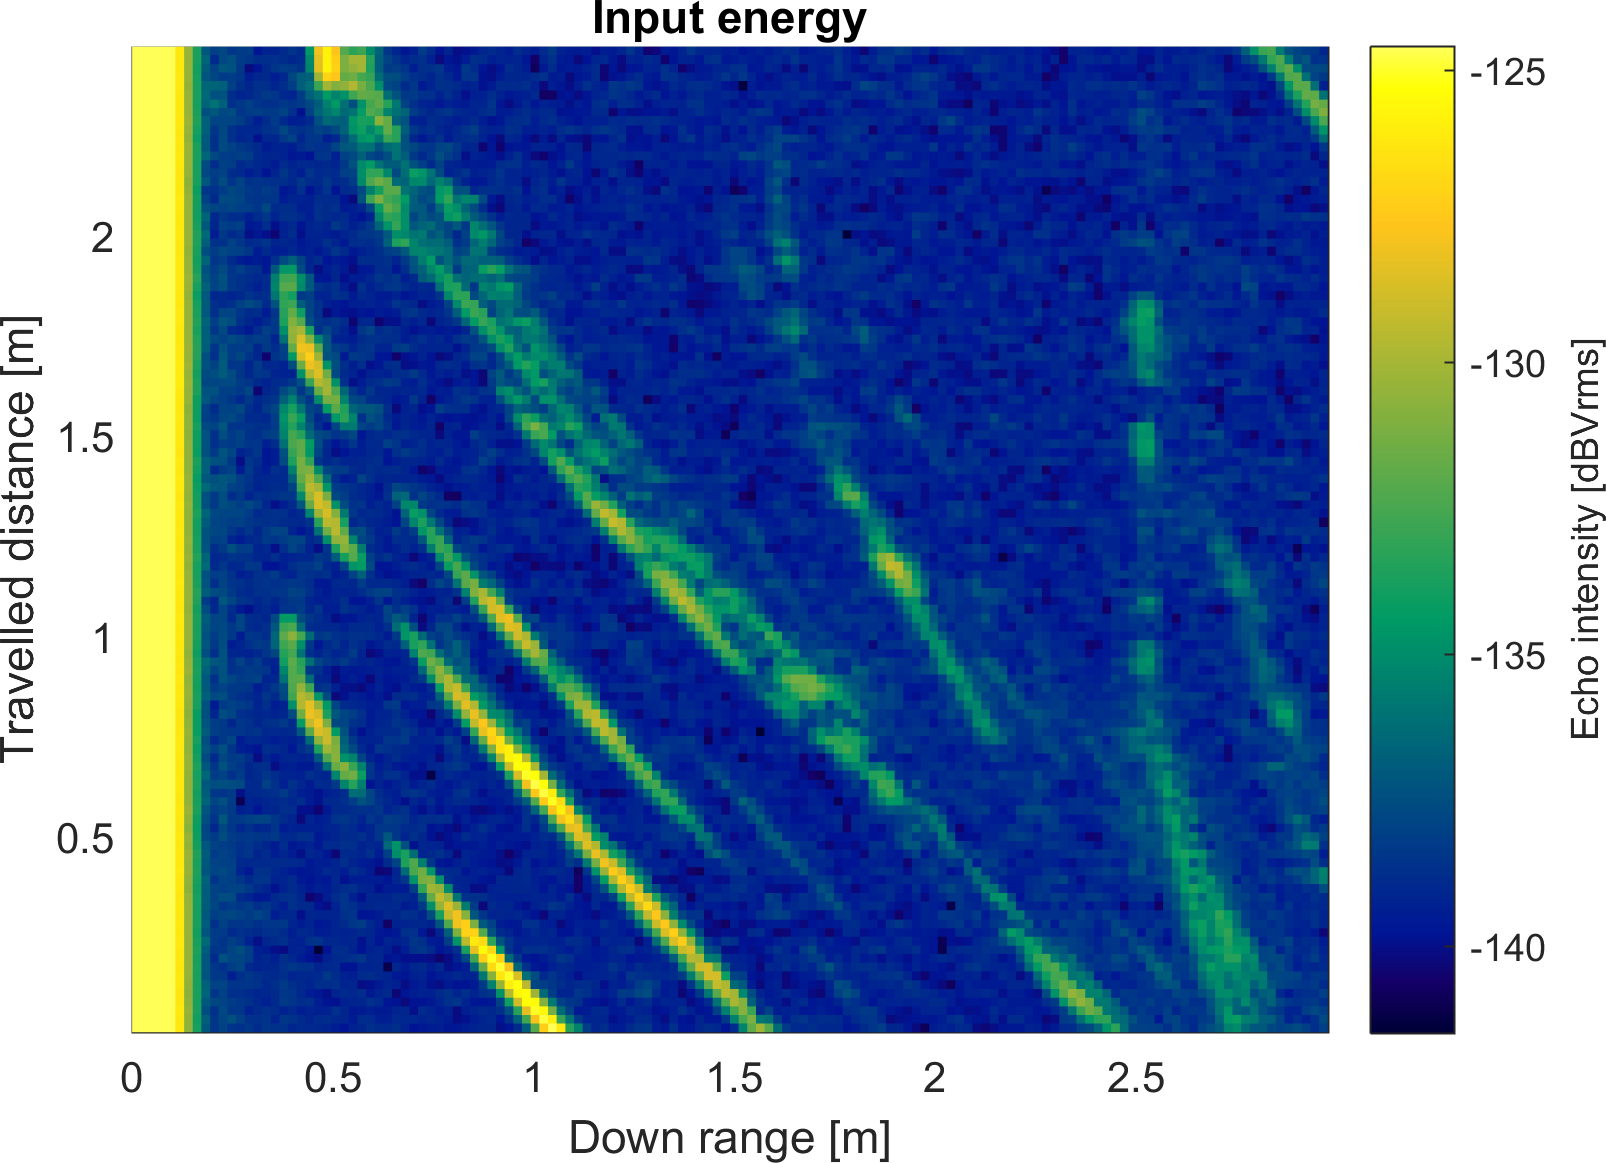
\includegraphics{gfx/results/falloutshelter_input}}     & \raisebox{-.5\height}{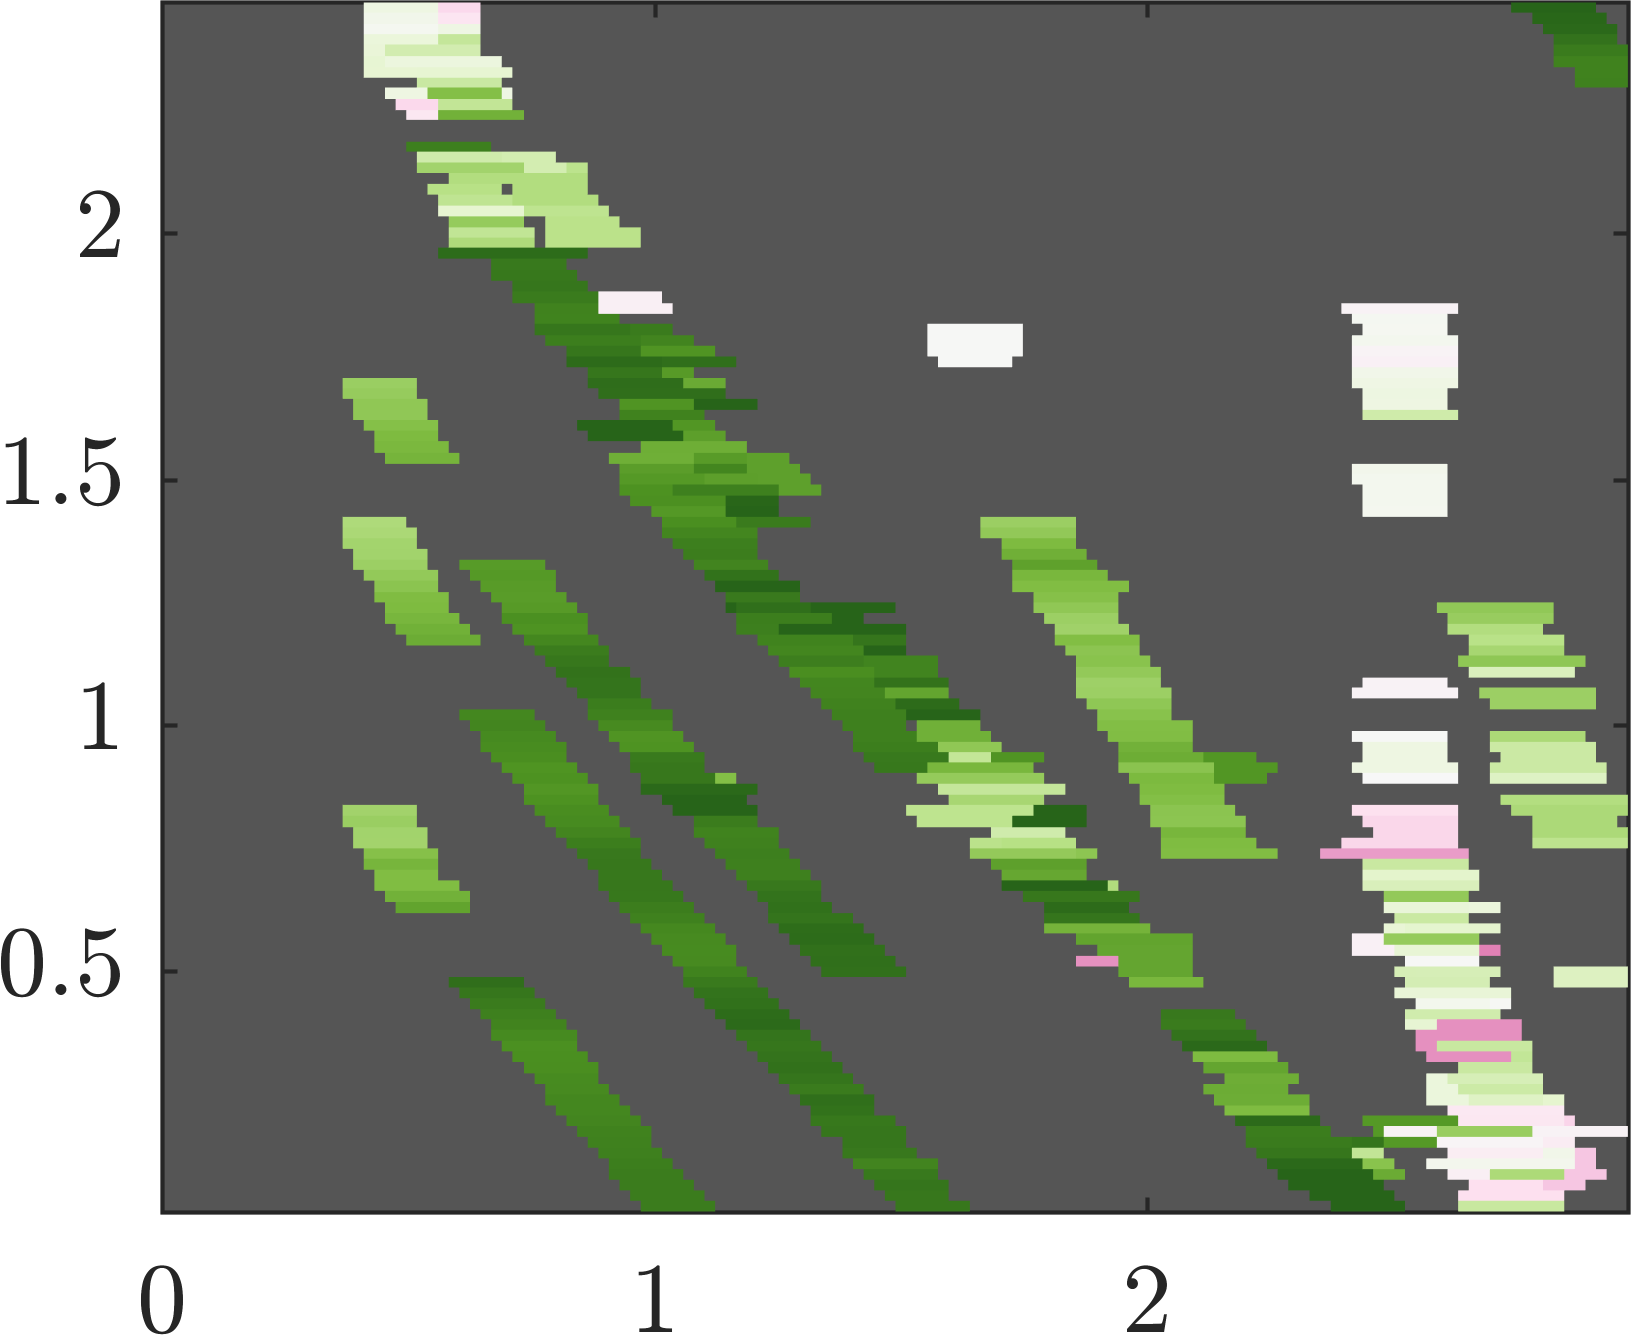
\includegraphics{gfx/results/falloutshelter_doppler}}     & \raisebox{-.5\height}{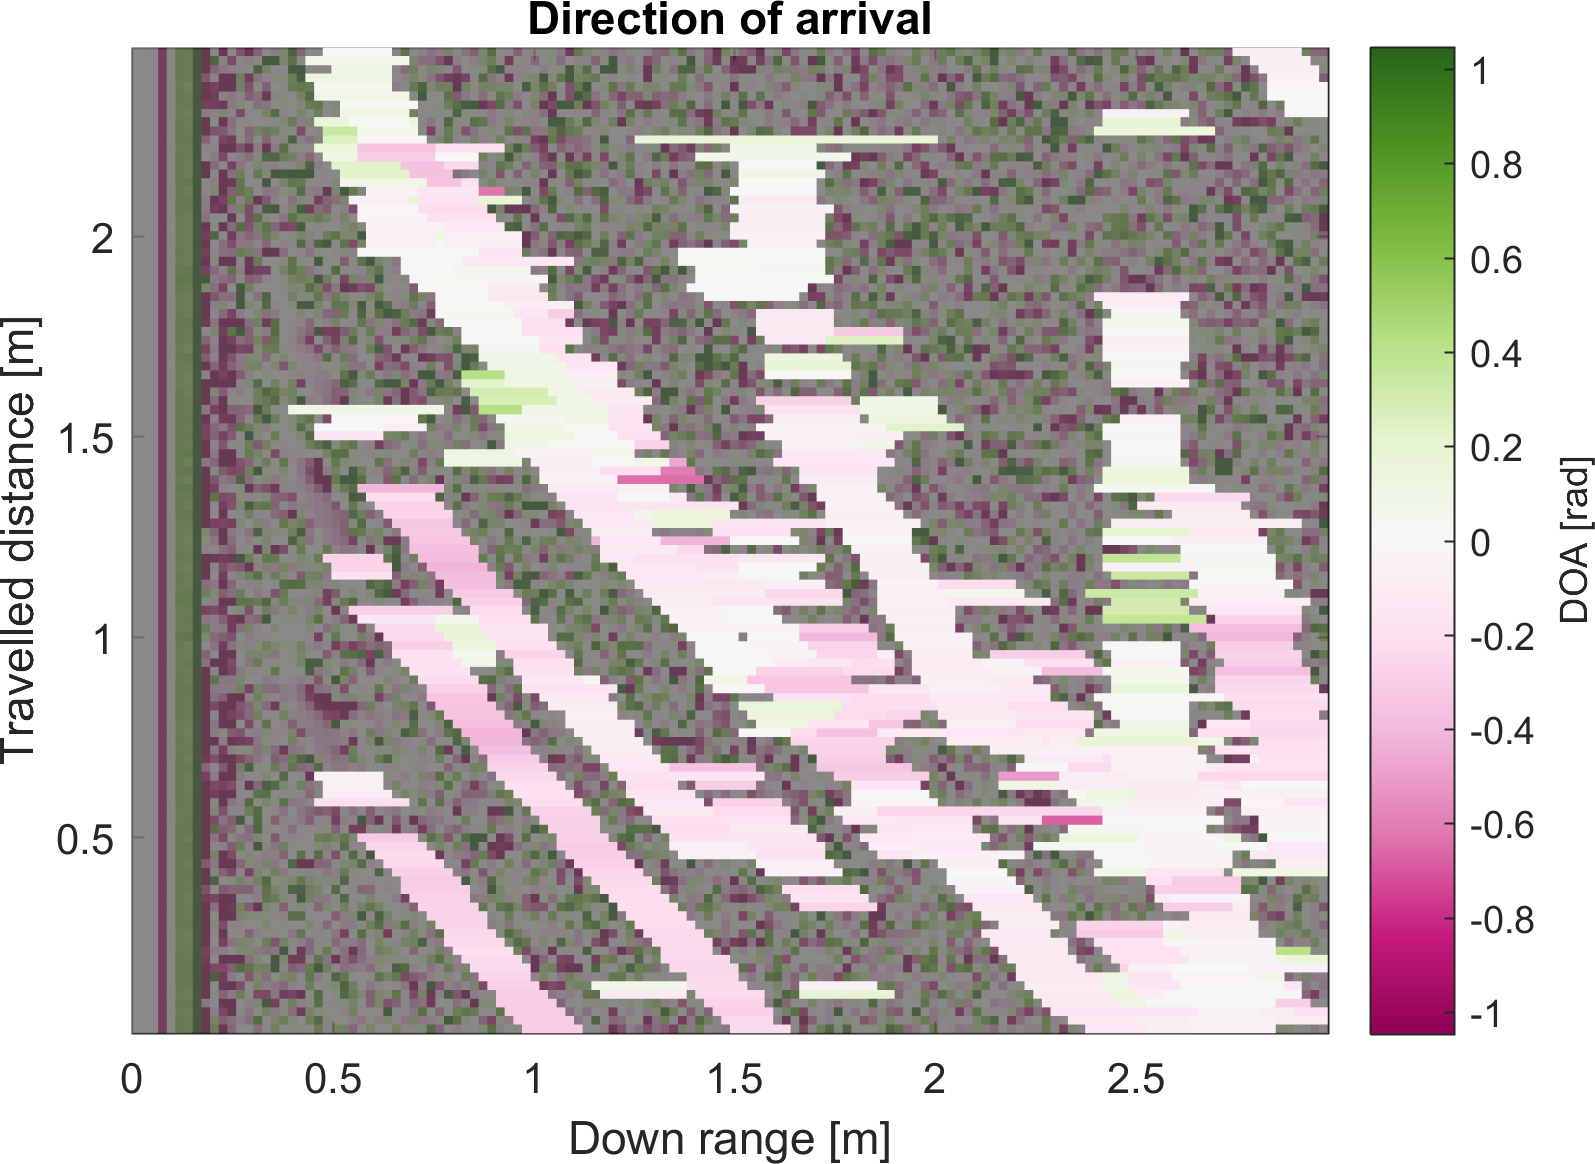
\includegraphics{gfx/results/falloutshelter_doa}}     & \raisebox{-.5\height}{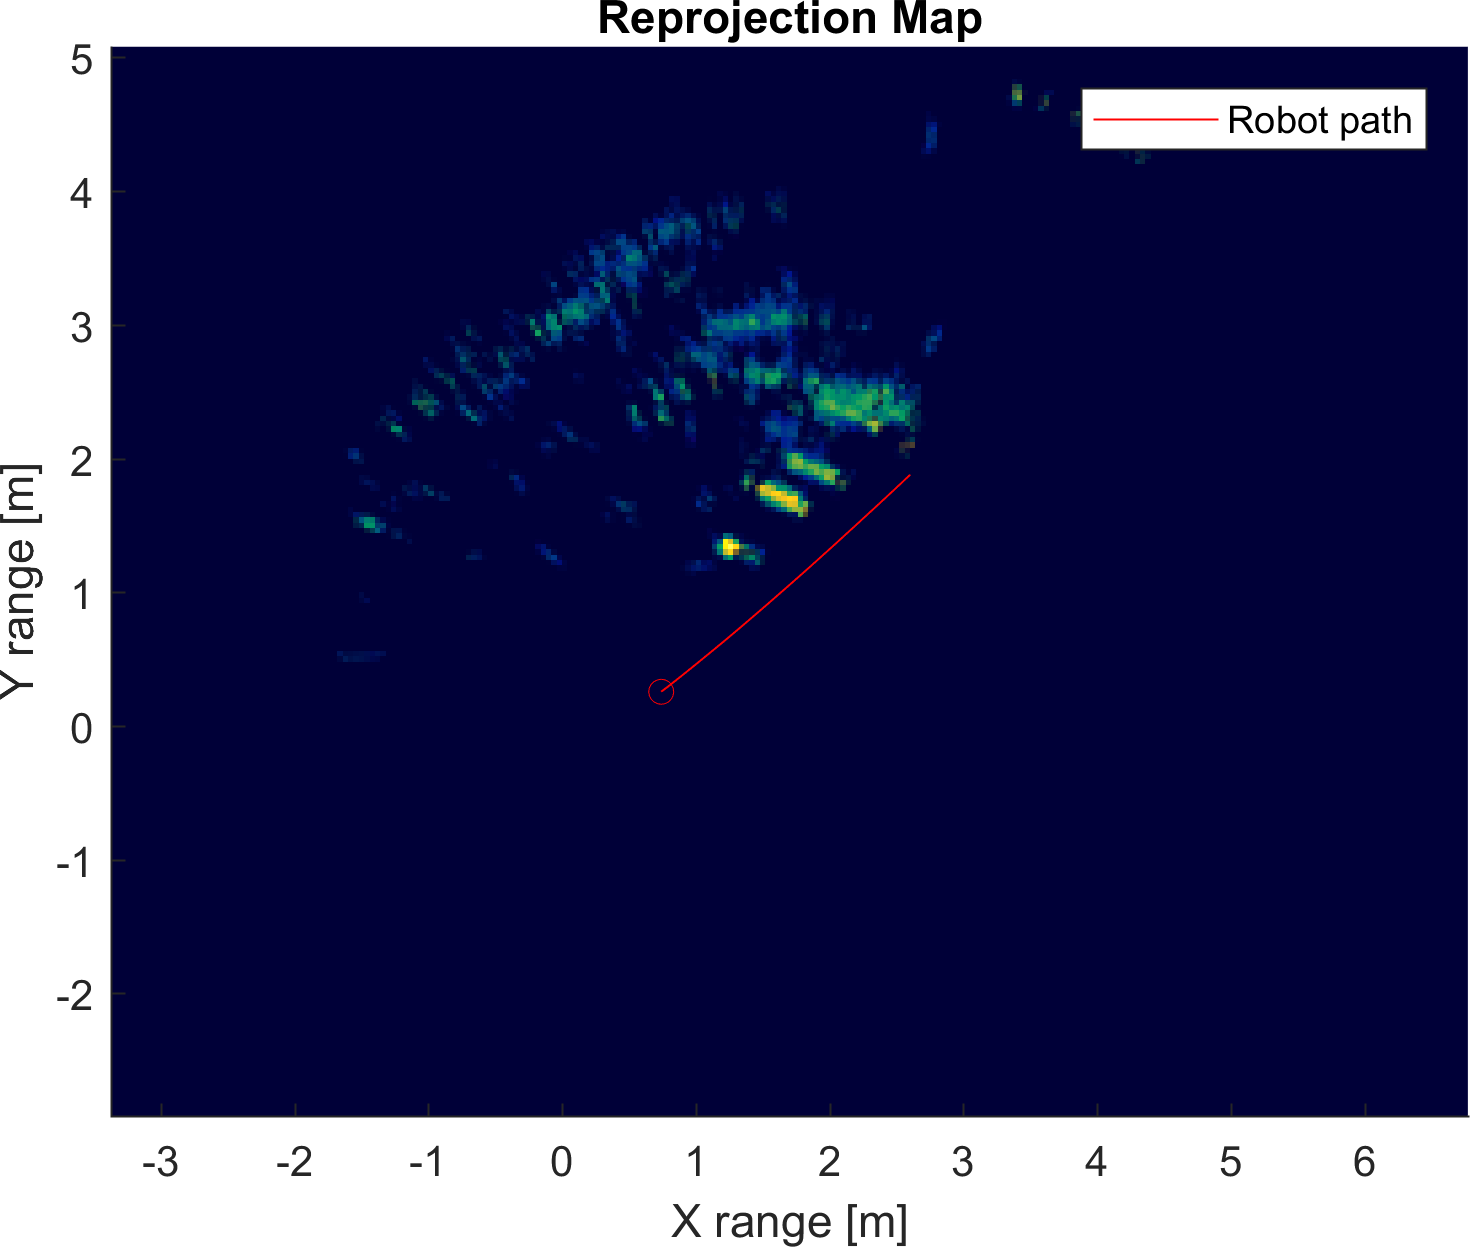
\includegraphics{gfx/results/falloutshelter_reprojection}}     & 5ms        & V           & 20°    & \cmark & \xmark & \xmark \\
% Garden                            & \raisebox{-.5\height}{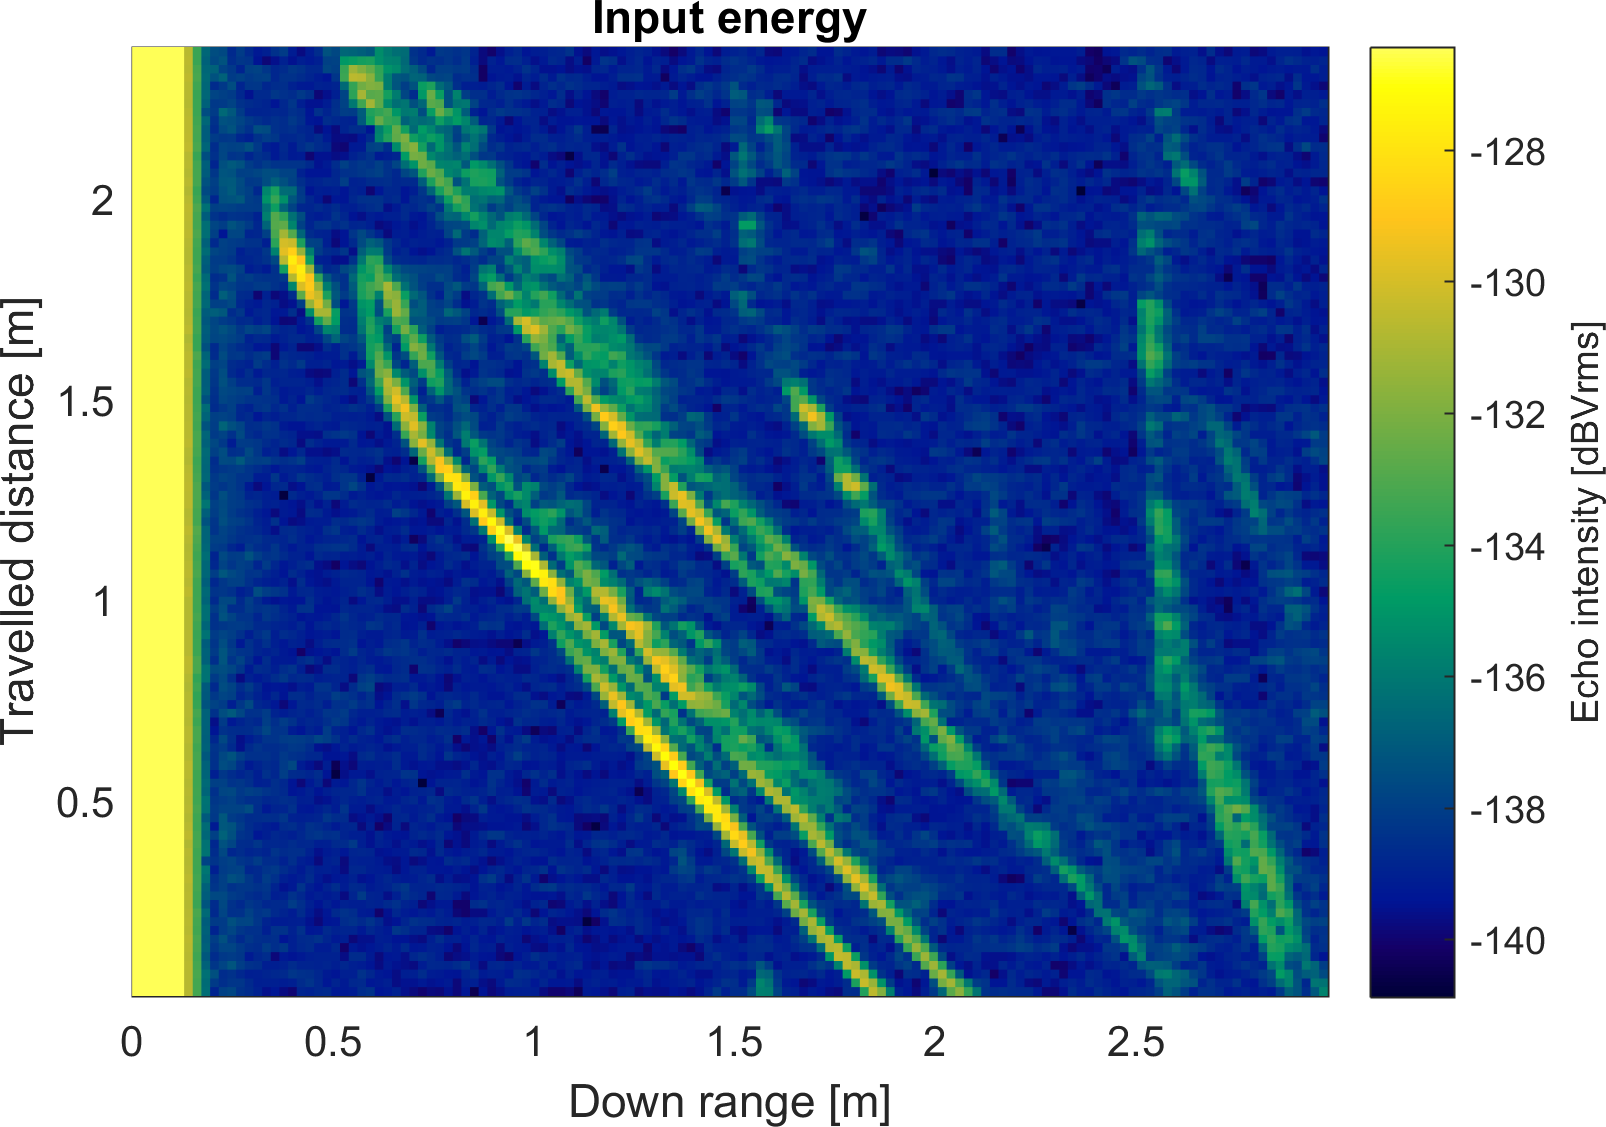
\includegraphics{gfx/results/garden_input}}             & \raisebox{-.5\height}{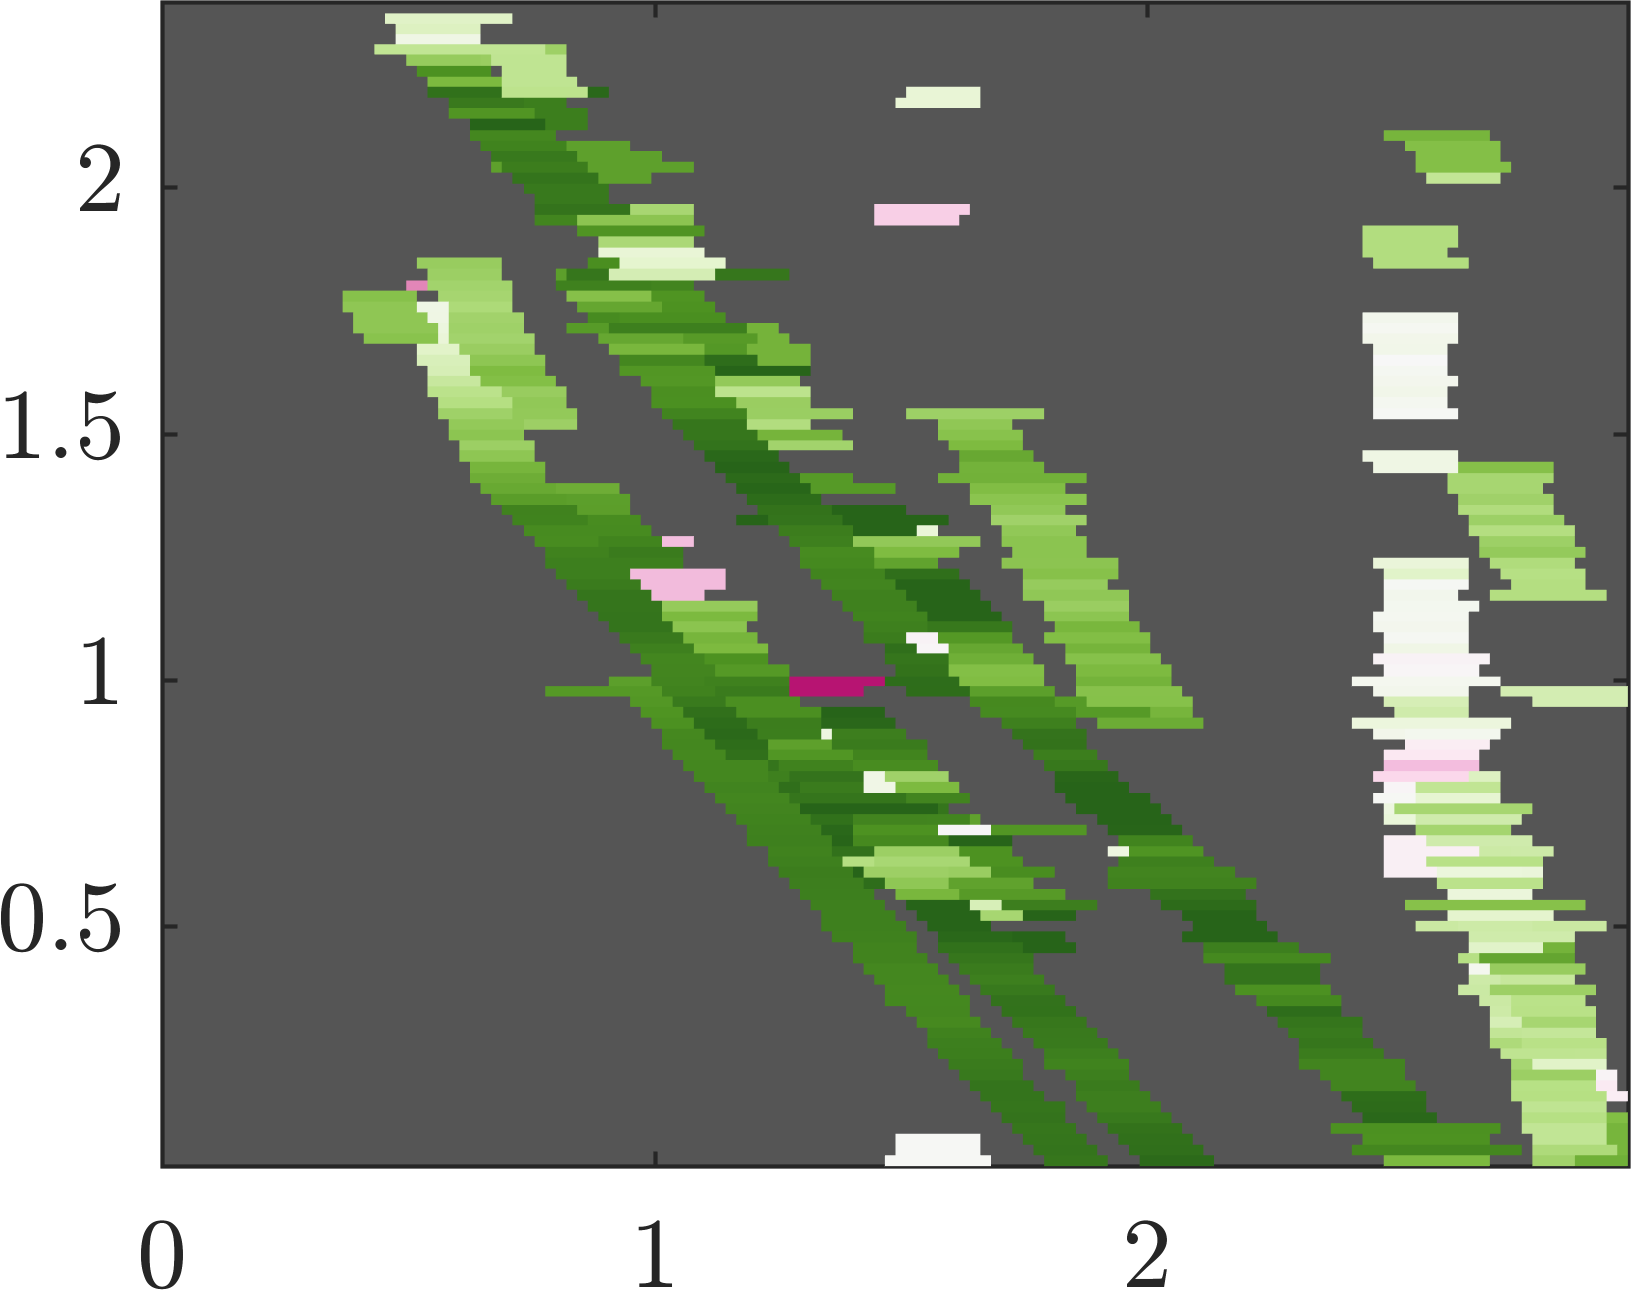
\includegraphics{gfx/results/garden_doppler}}             & \raisebox{-.5\height}{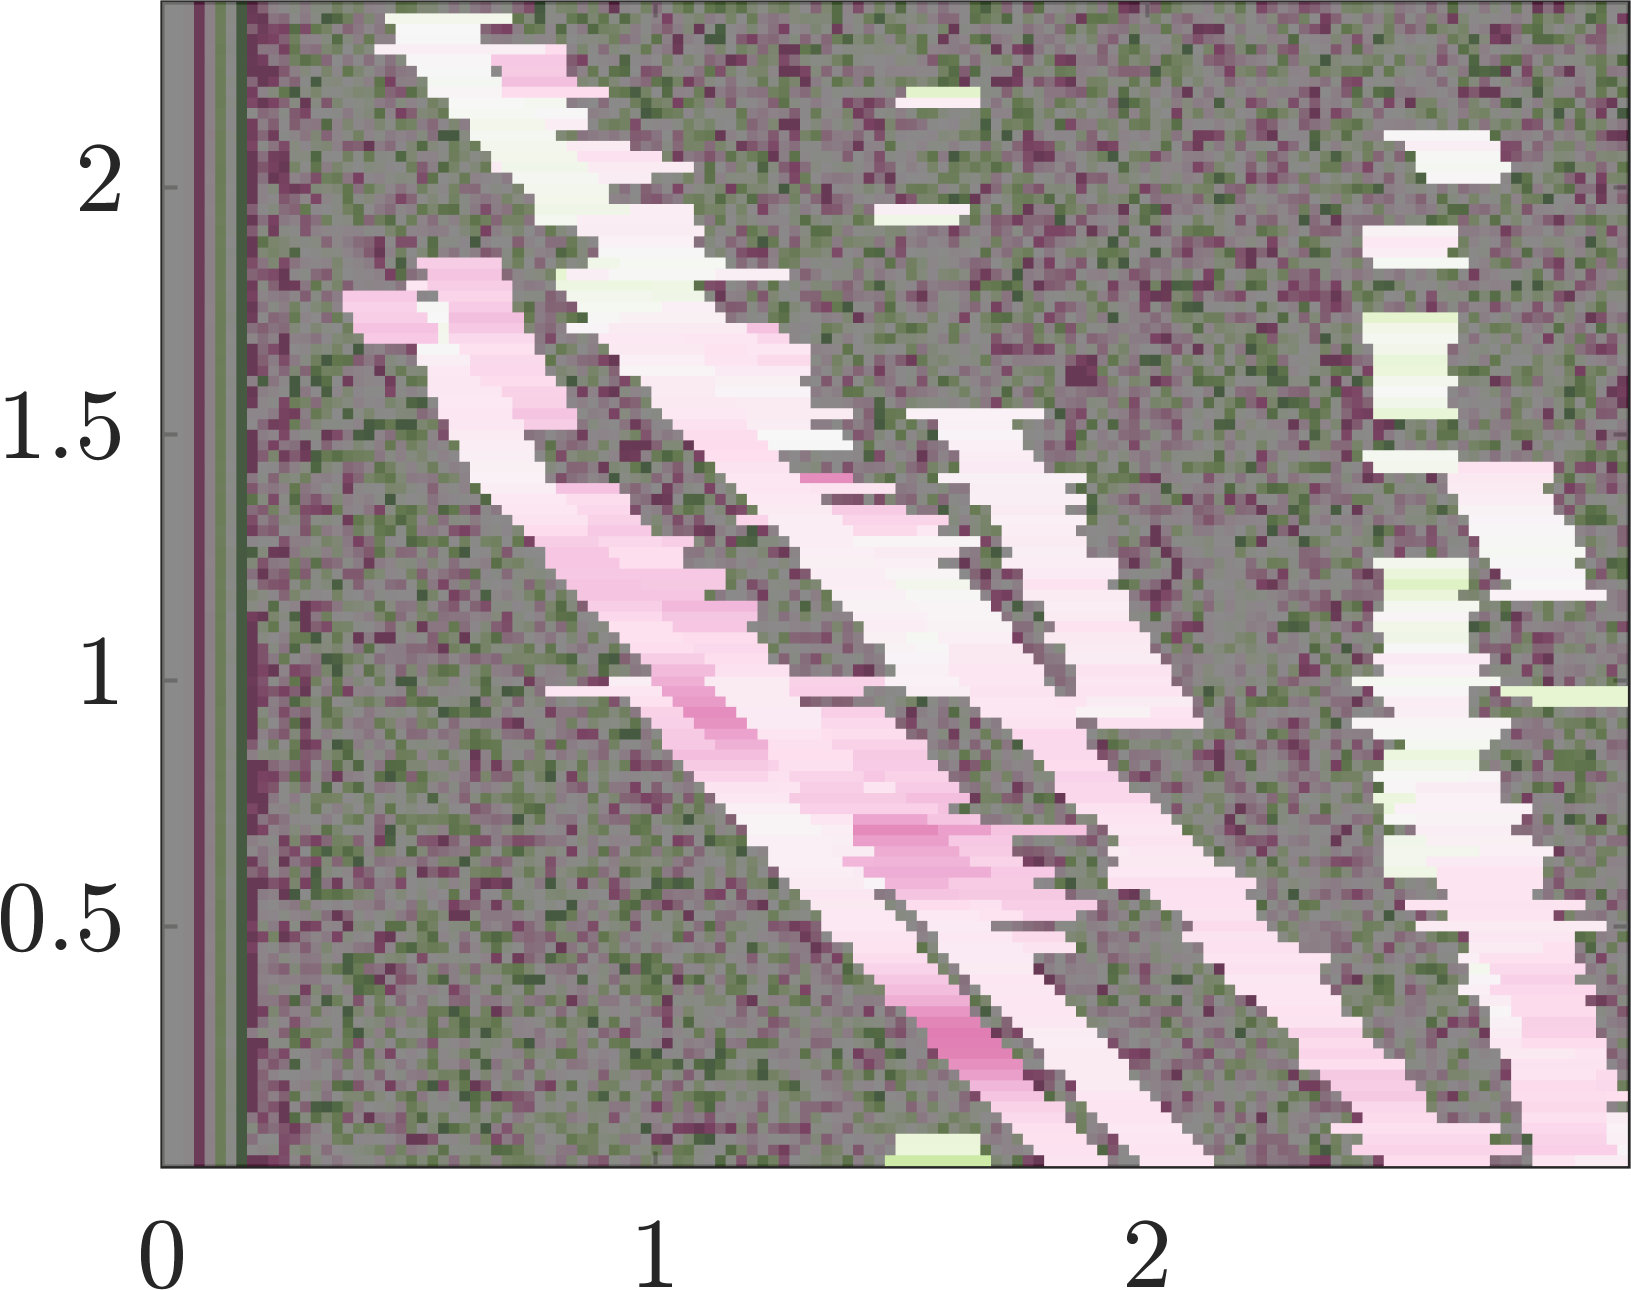
\includegraphics{gfx/results/garden_doa}}             & \raisebox{-.5\height}{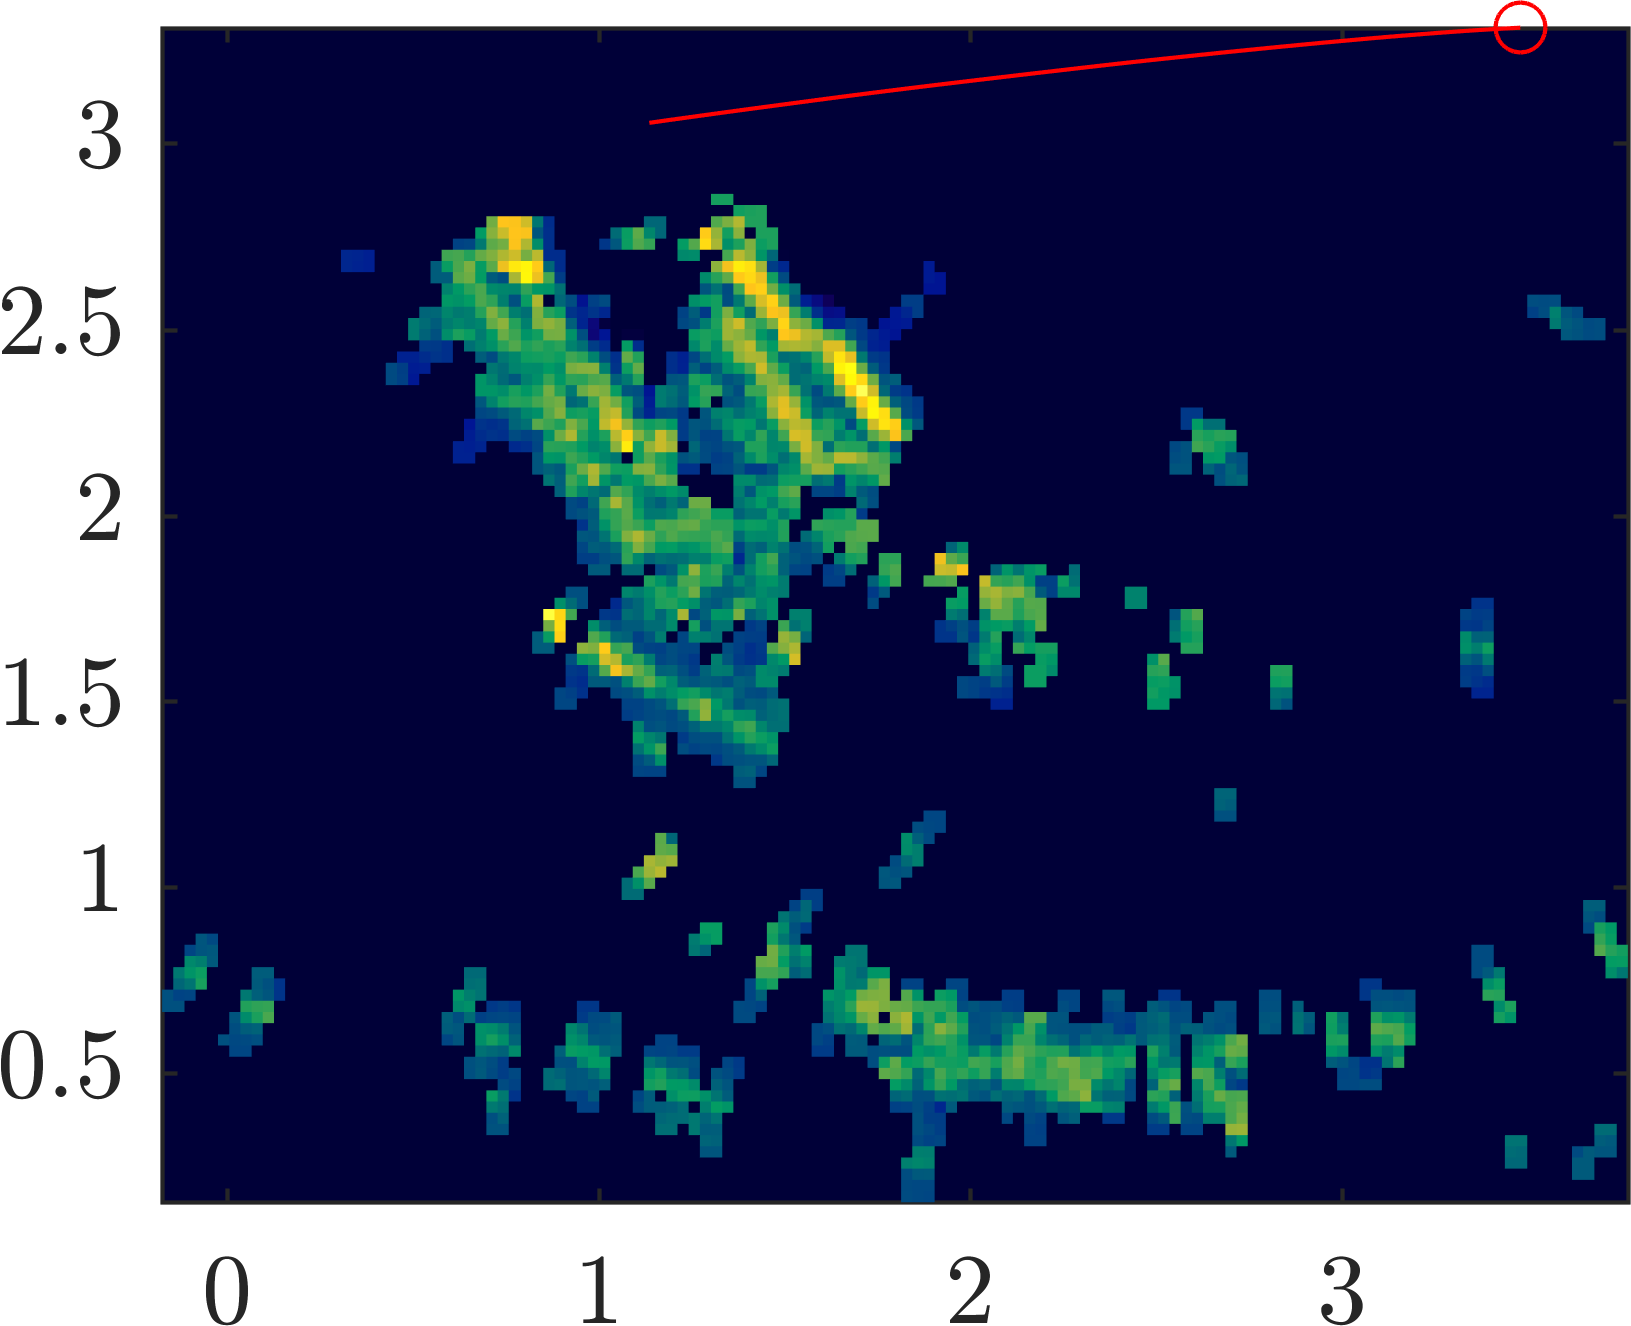
\includegraphics{gfx/results/garden_reprojection}}             & 5ms        & V           & 20°    & \cmark & \xmark & \xmark \\
% Home cinema                       & \raisebox{-.5\height}{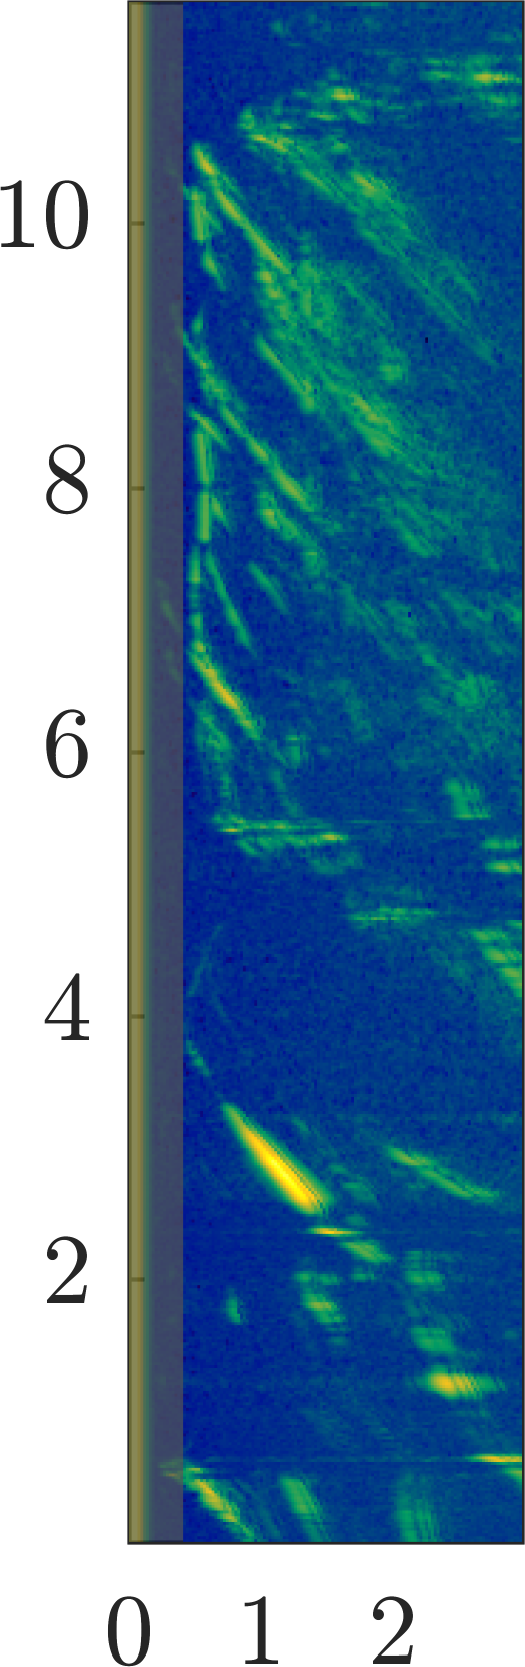
\includegraphics{gfx/results/homecinema_input}}         & \raisebox{-.5\height}{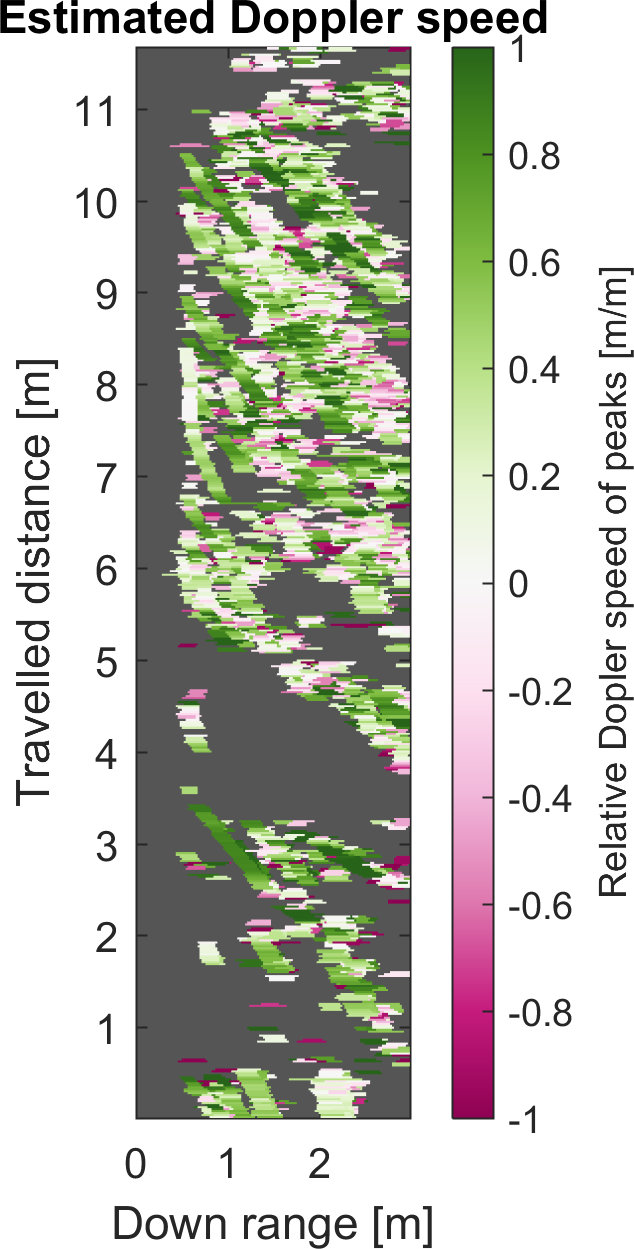
\includegraphics{gfx/results/homecinema_doppler}}         & \raisebox{-.5\height}{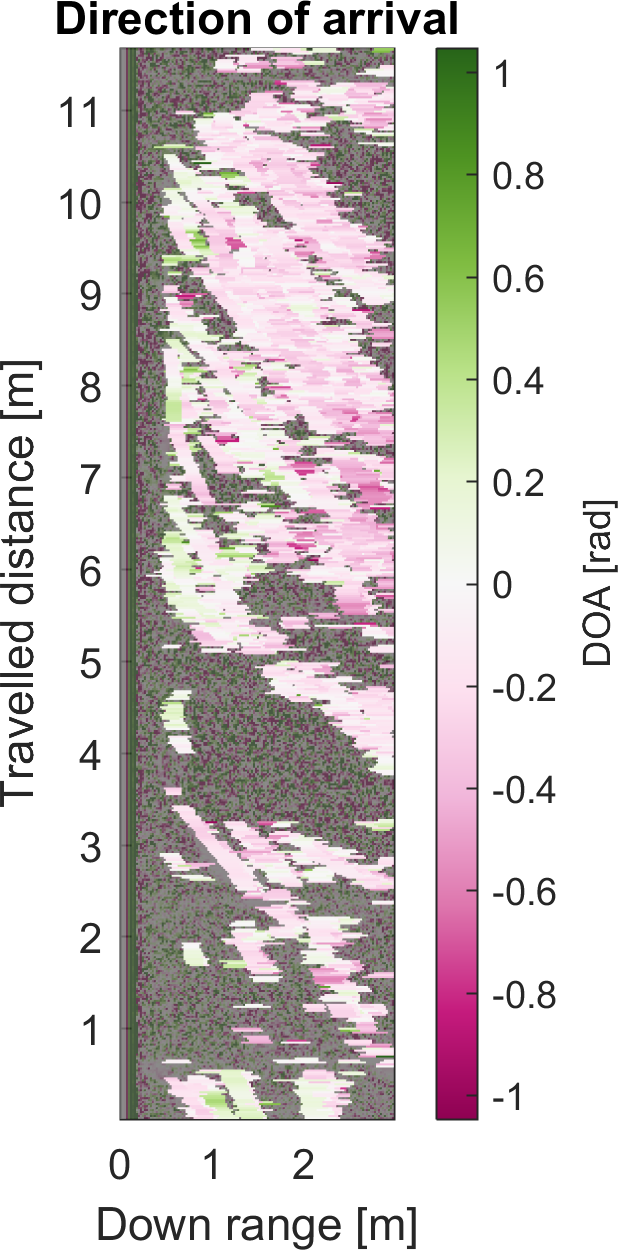
\includegraphics{gfx/results/homecinema_doa}}         & \raisebox{-.5\height}{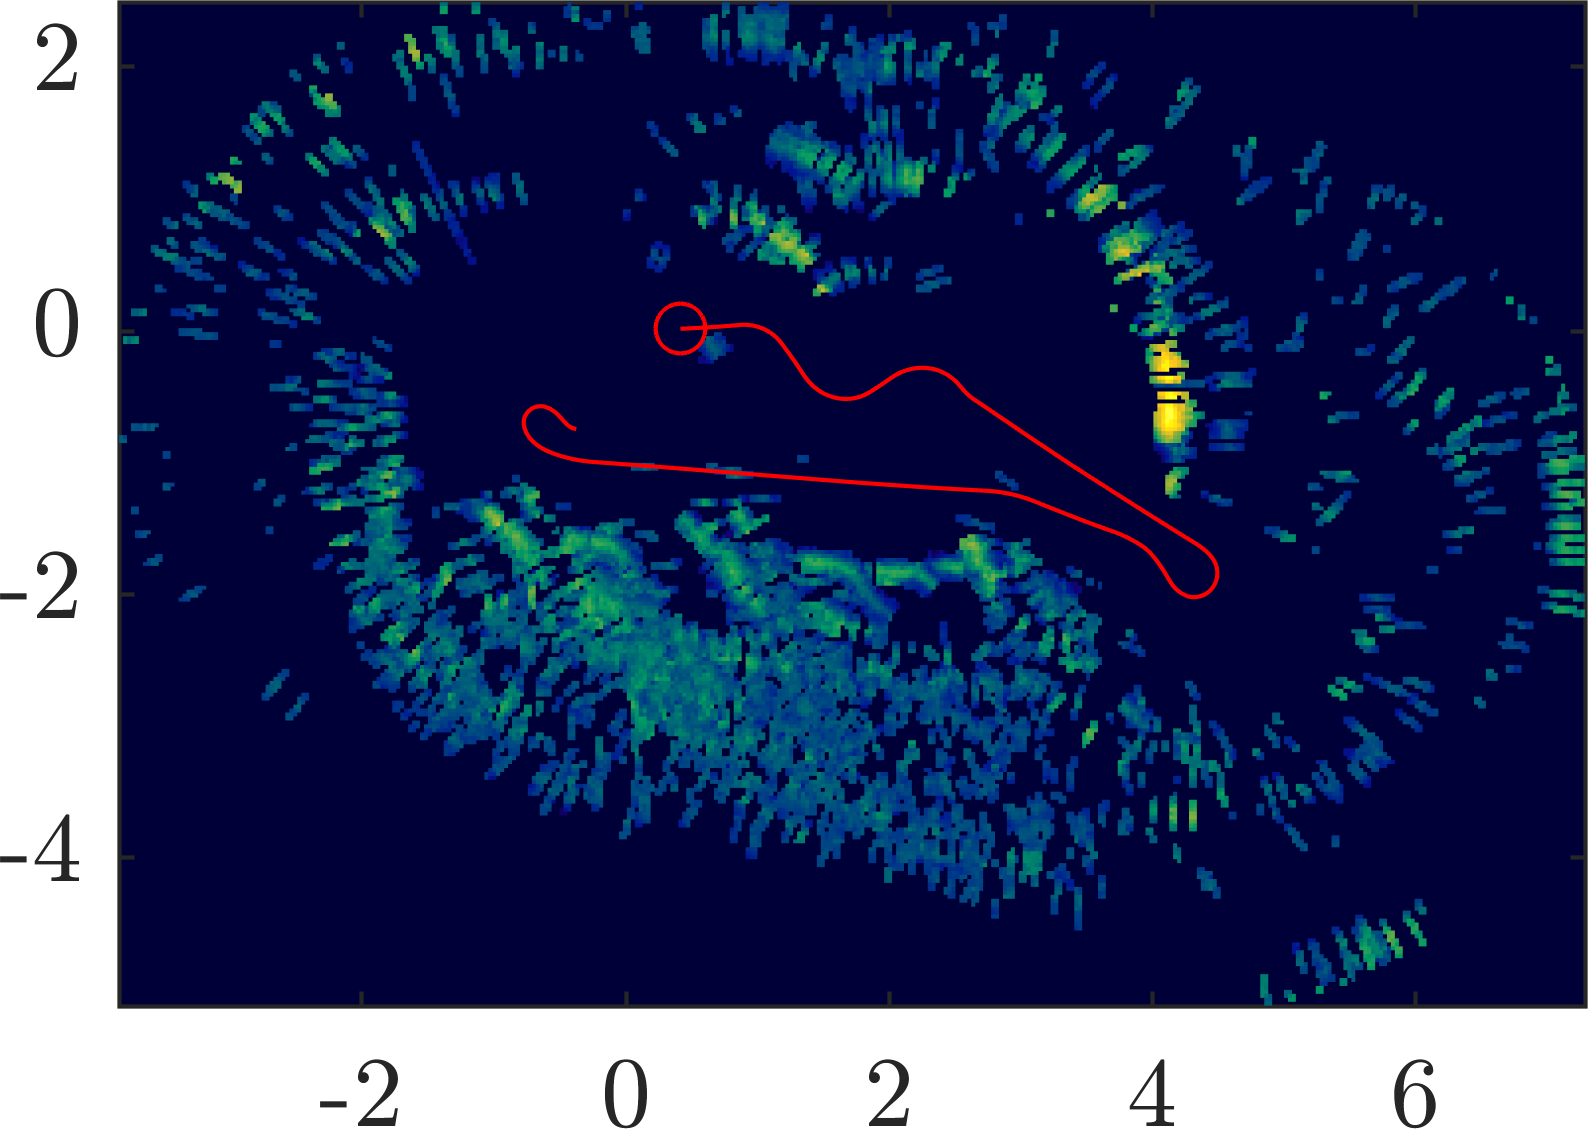
\includegraphics{gfx/results/homecinema_reprojection}}         & 5ms        & V           & 20°    & \cmark & \xmark & \xmark \\
% Indoor swimming pool              & \raisebox{-.5\height}{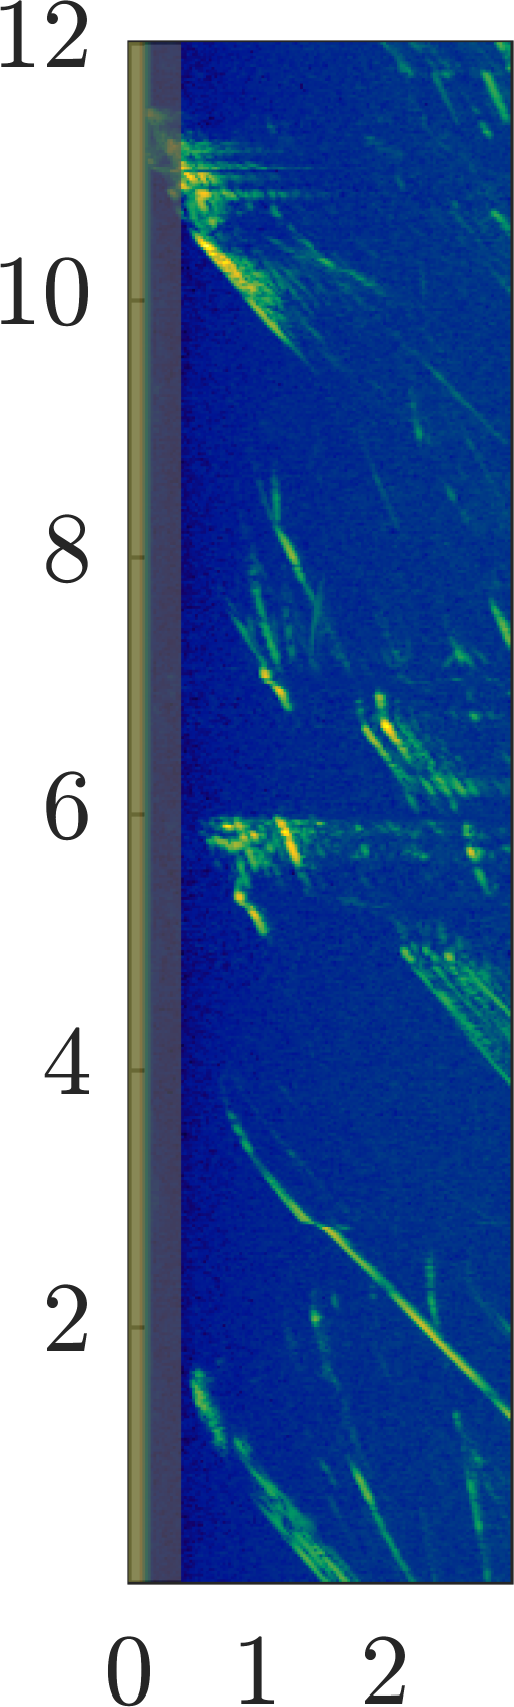
\includegraphics{gfx/results/indoorswimmingpool_input}} & \raisebox{-.5\height}{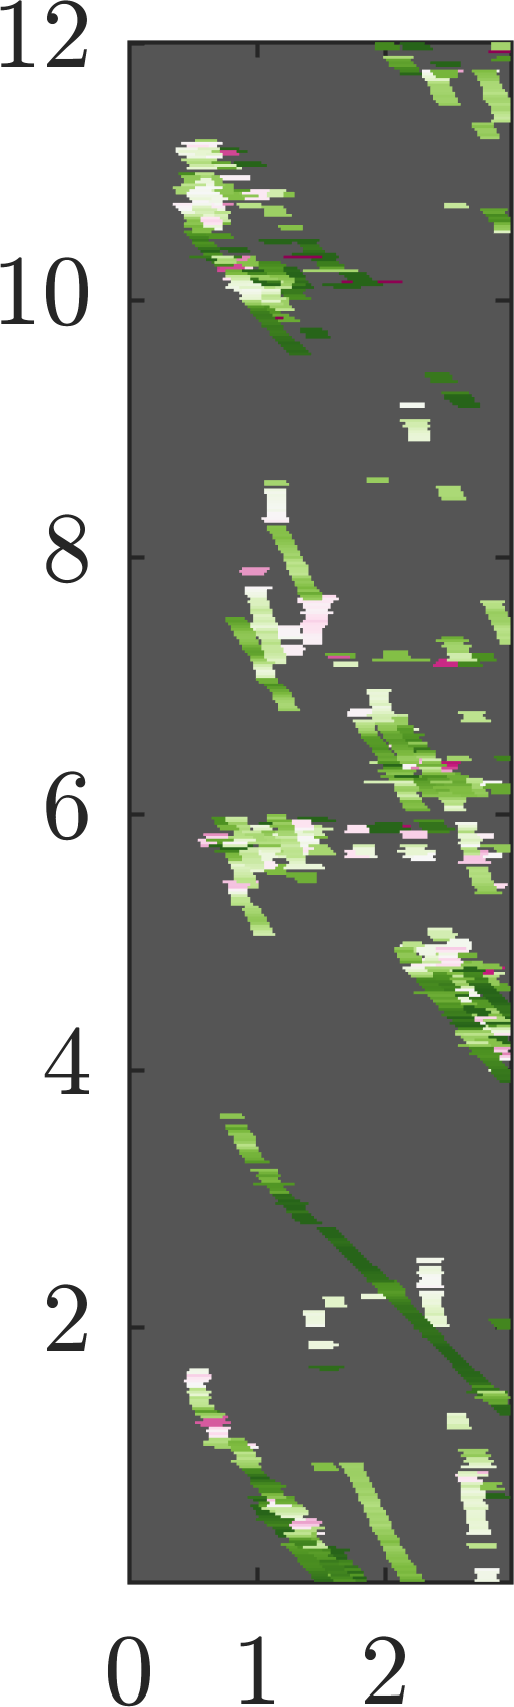
\includegraphics{gfx/results/indoorswimmingpool_doppler}} & \raisebox{-.5\height}{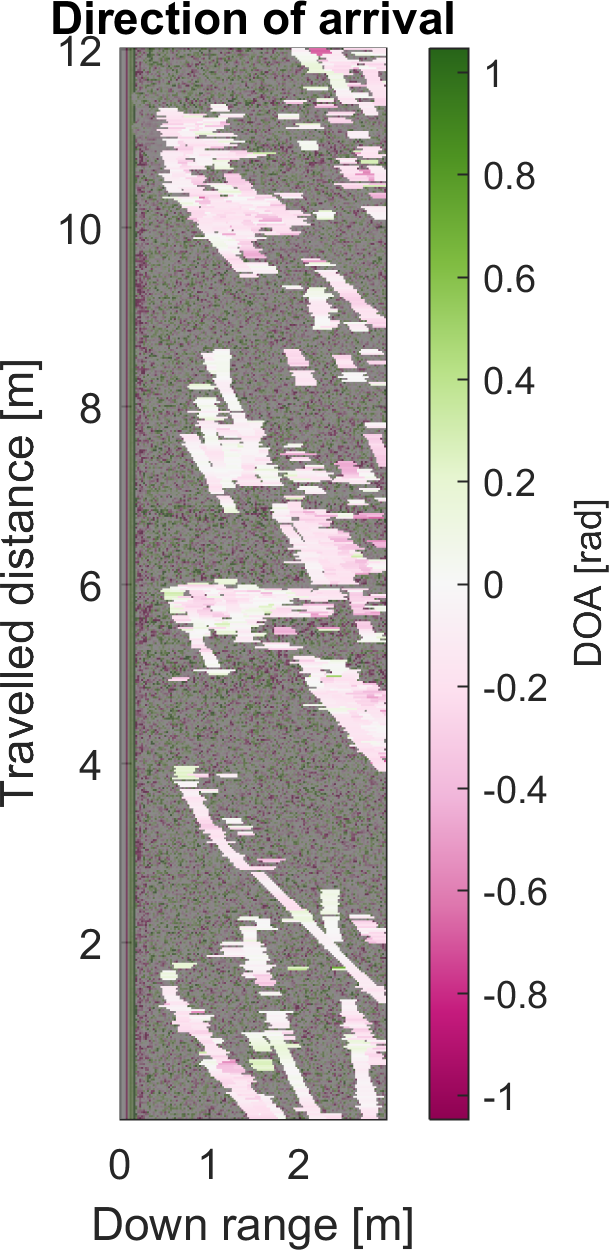
\includegraphics{gfx/results/indoorswimmingpool_doa}} & \raisebox{-.5\height}{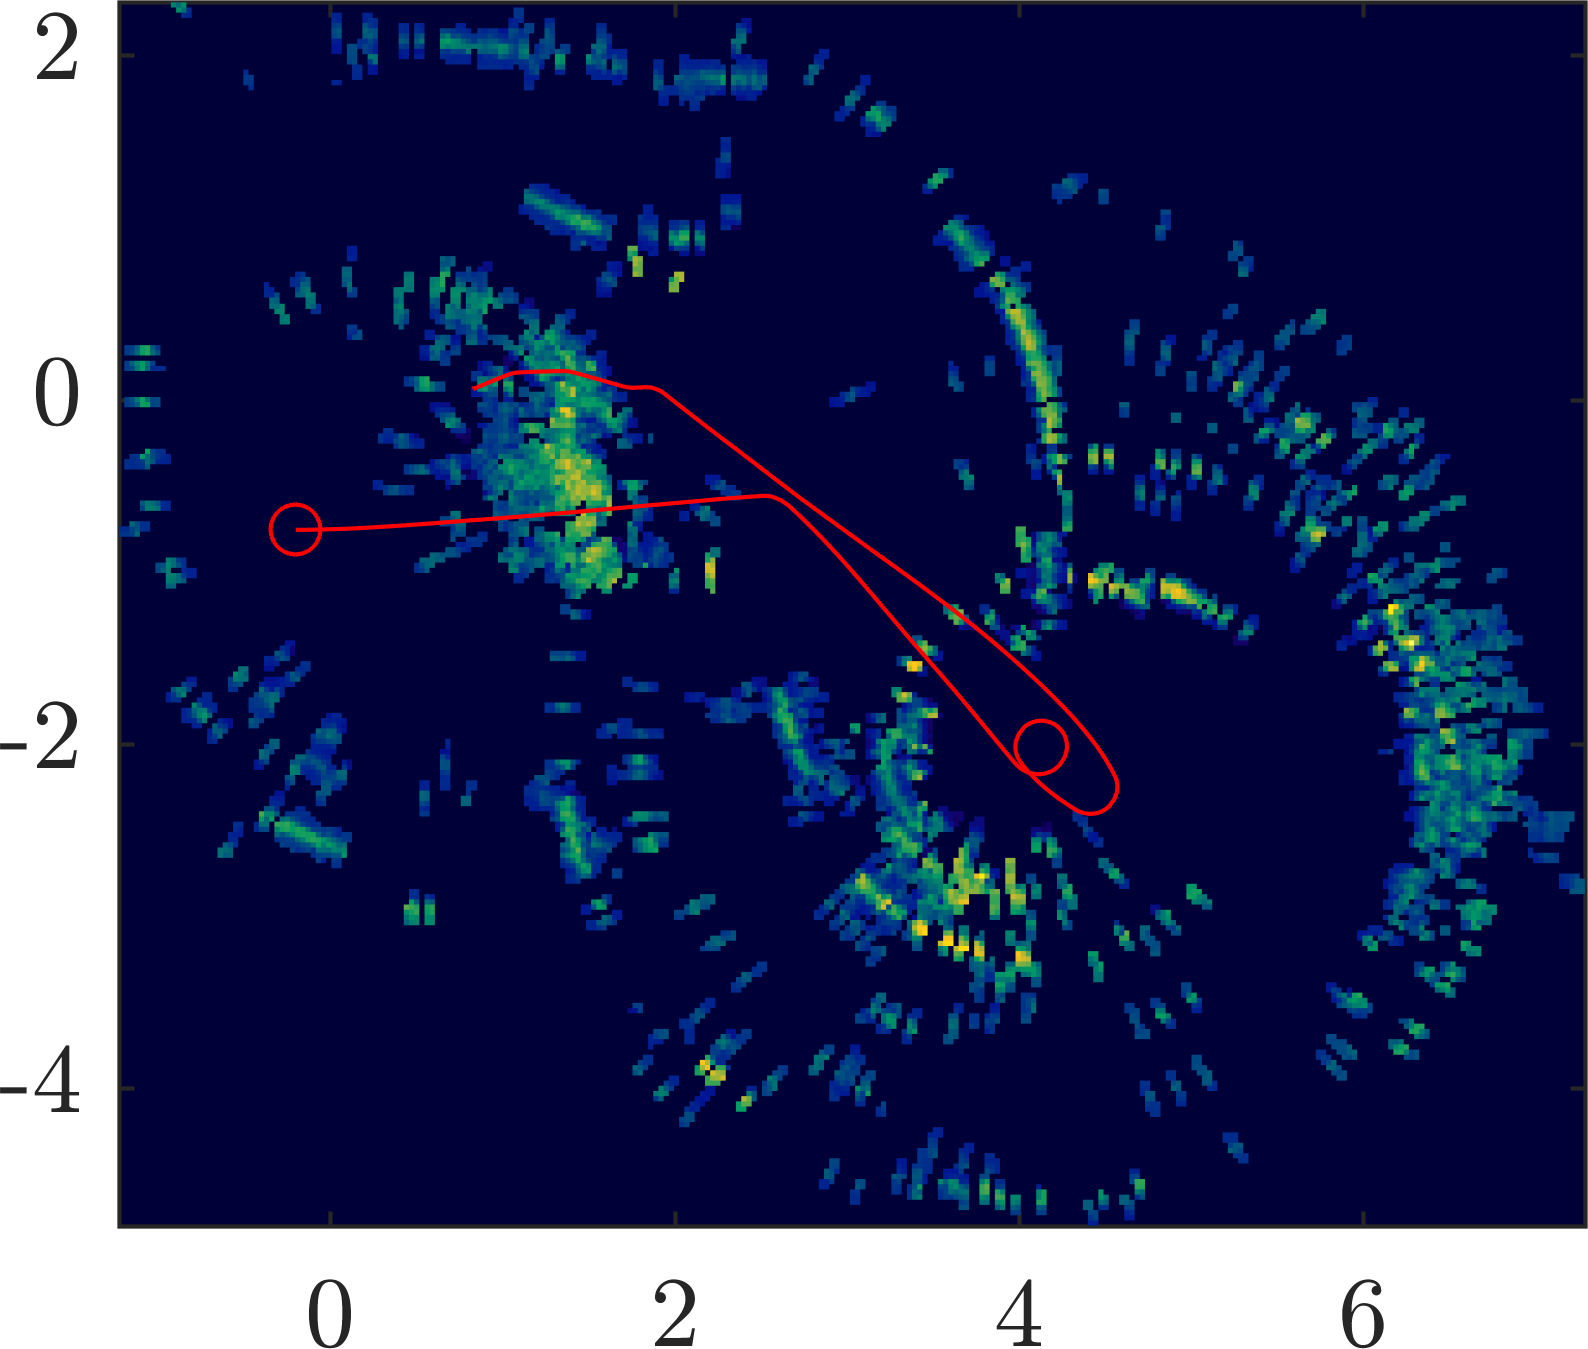
\includegraphics{gfx/results/indoorswimmingpool_reprojection}} & 5ms        & V           & 20°    & \cmark & \xmark & \xmark \\
% Jail cell                         & \raisebox{-.5\height}{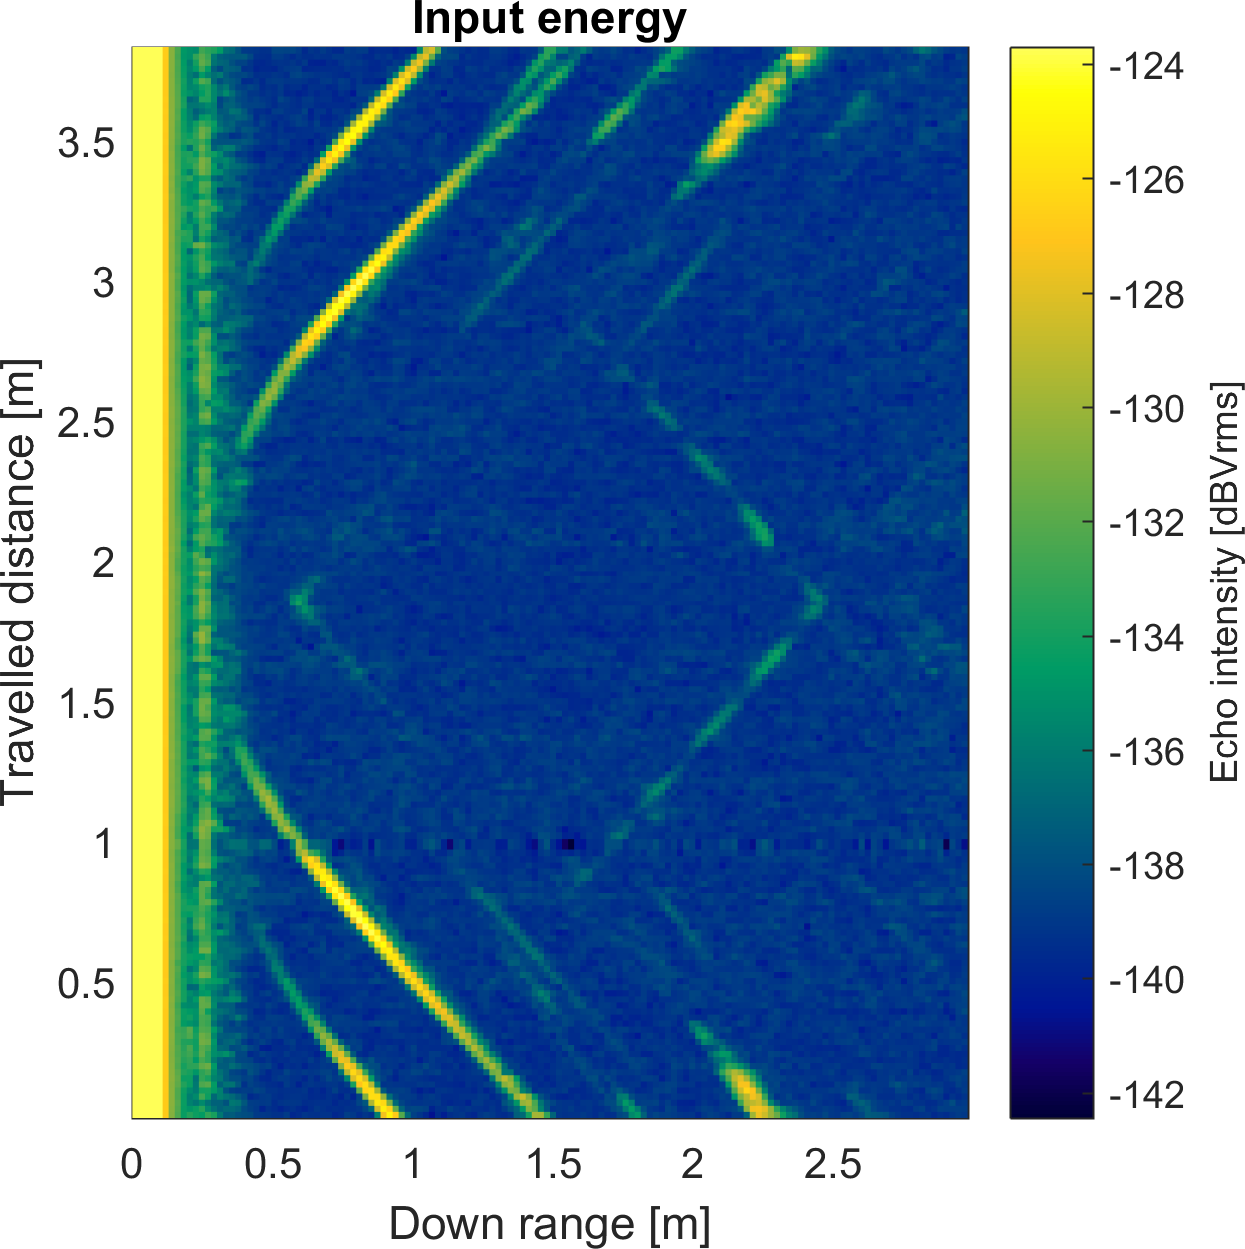
\includegraphics{gfx/results/jailcell_input}}           & \raisebox{-.5\height}{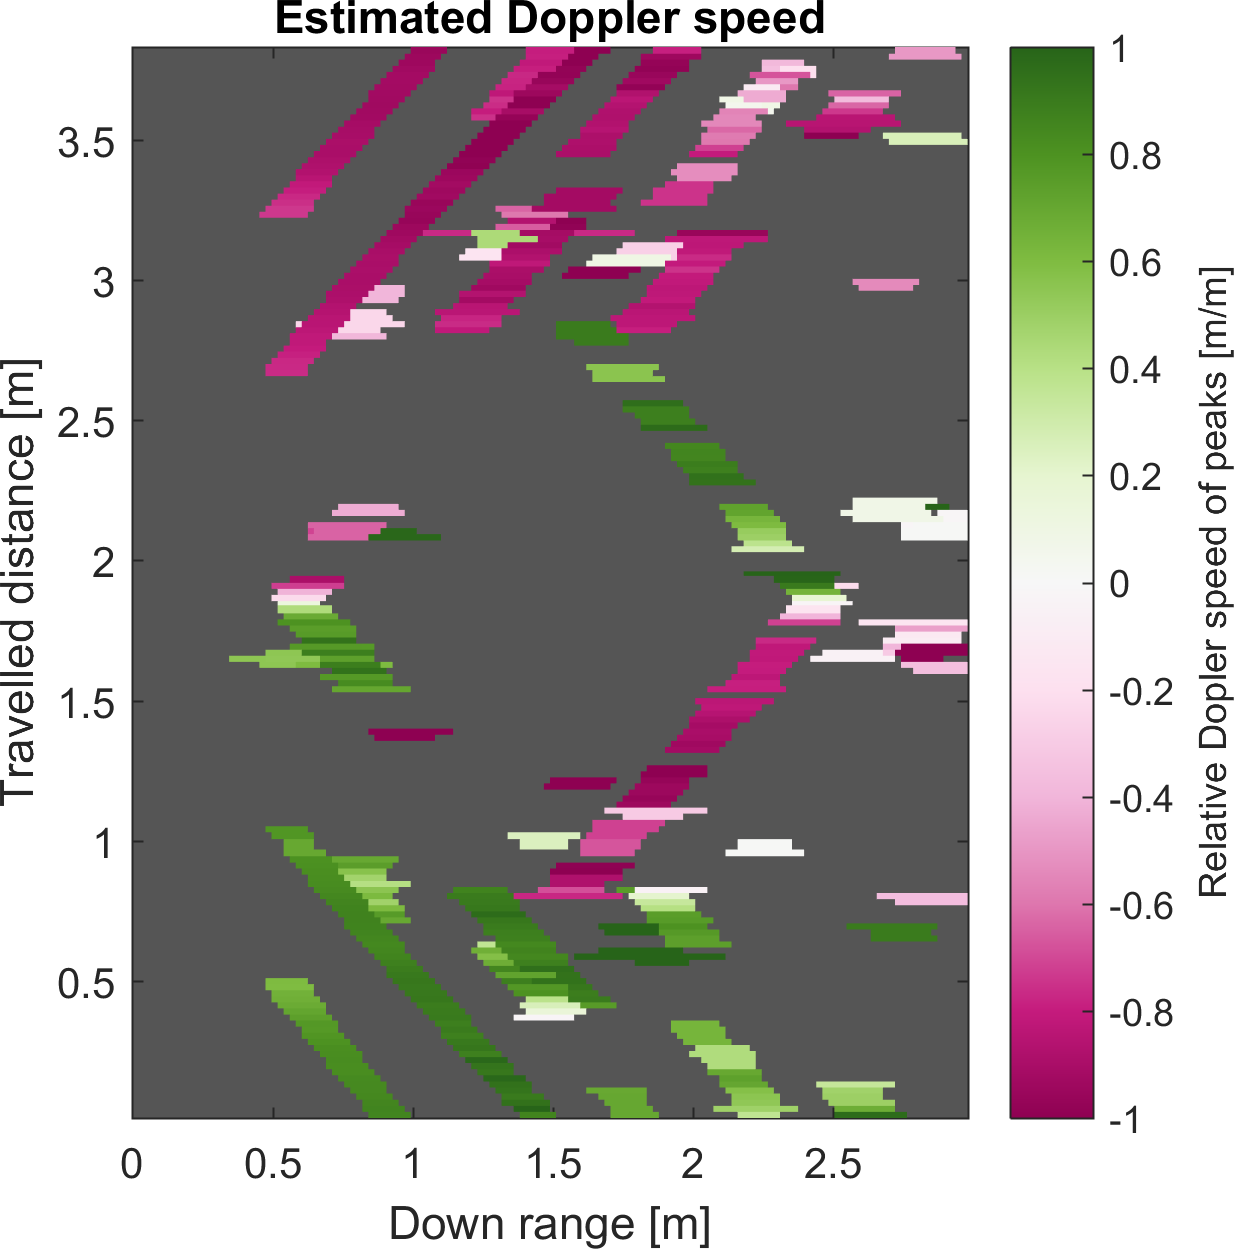
\includegraphics{gfx/results/jailcell_doppler}}           & \raisebox{-.5\height}{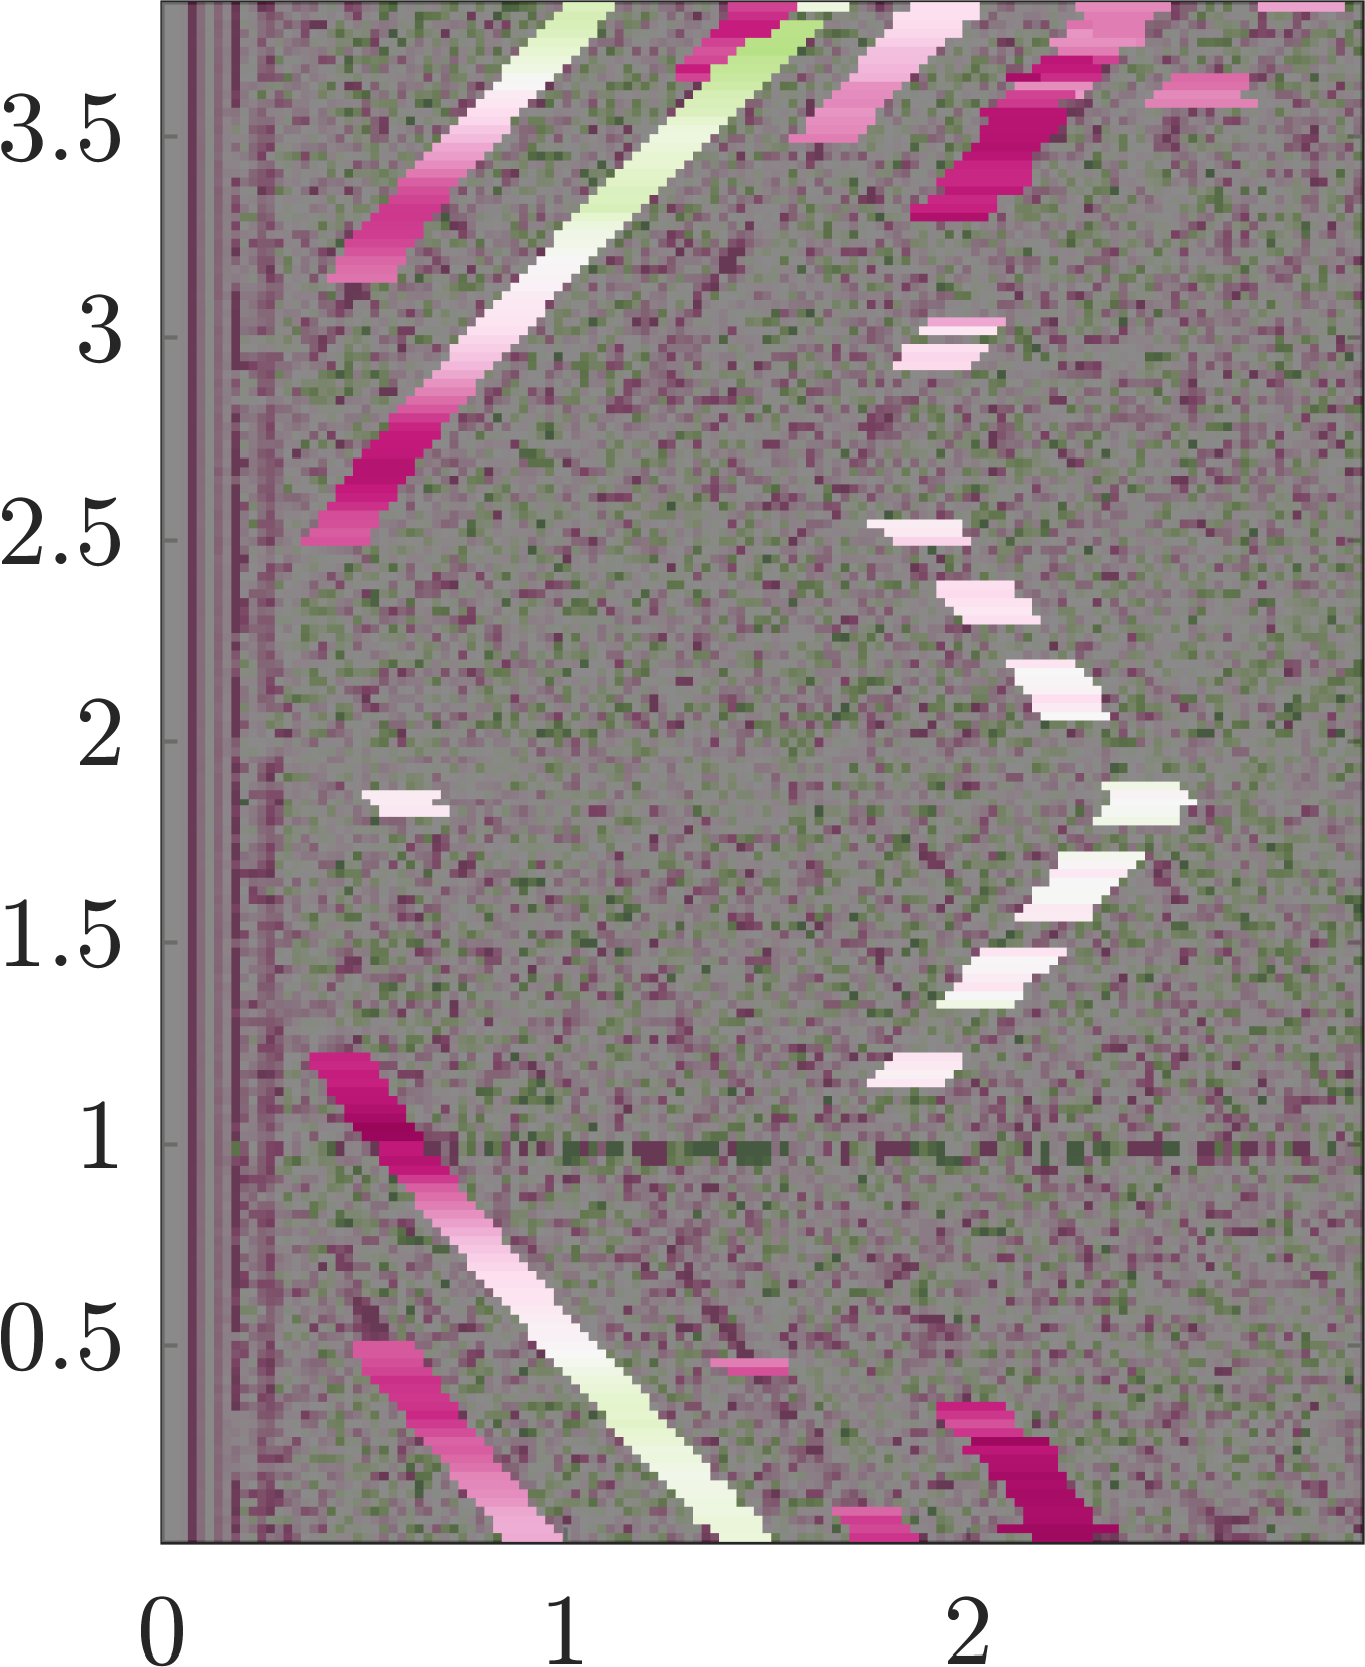
\includegraphics{gfx/results/jailcell_doa}}           & \raisebox{-.5\height}{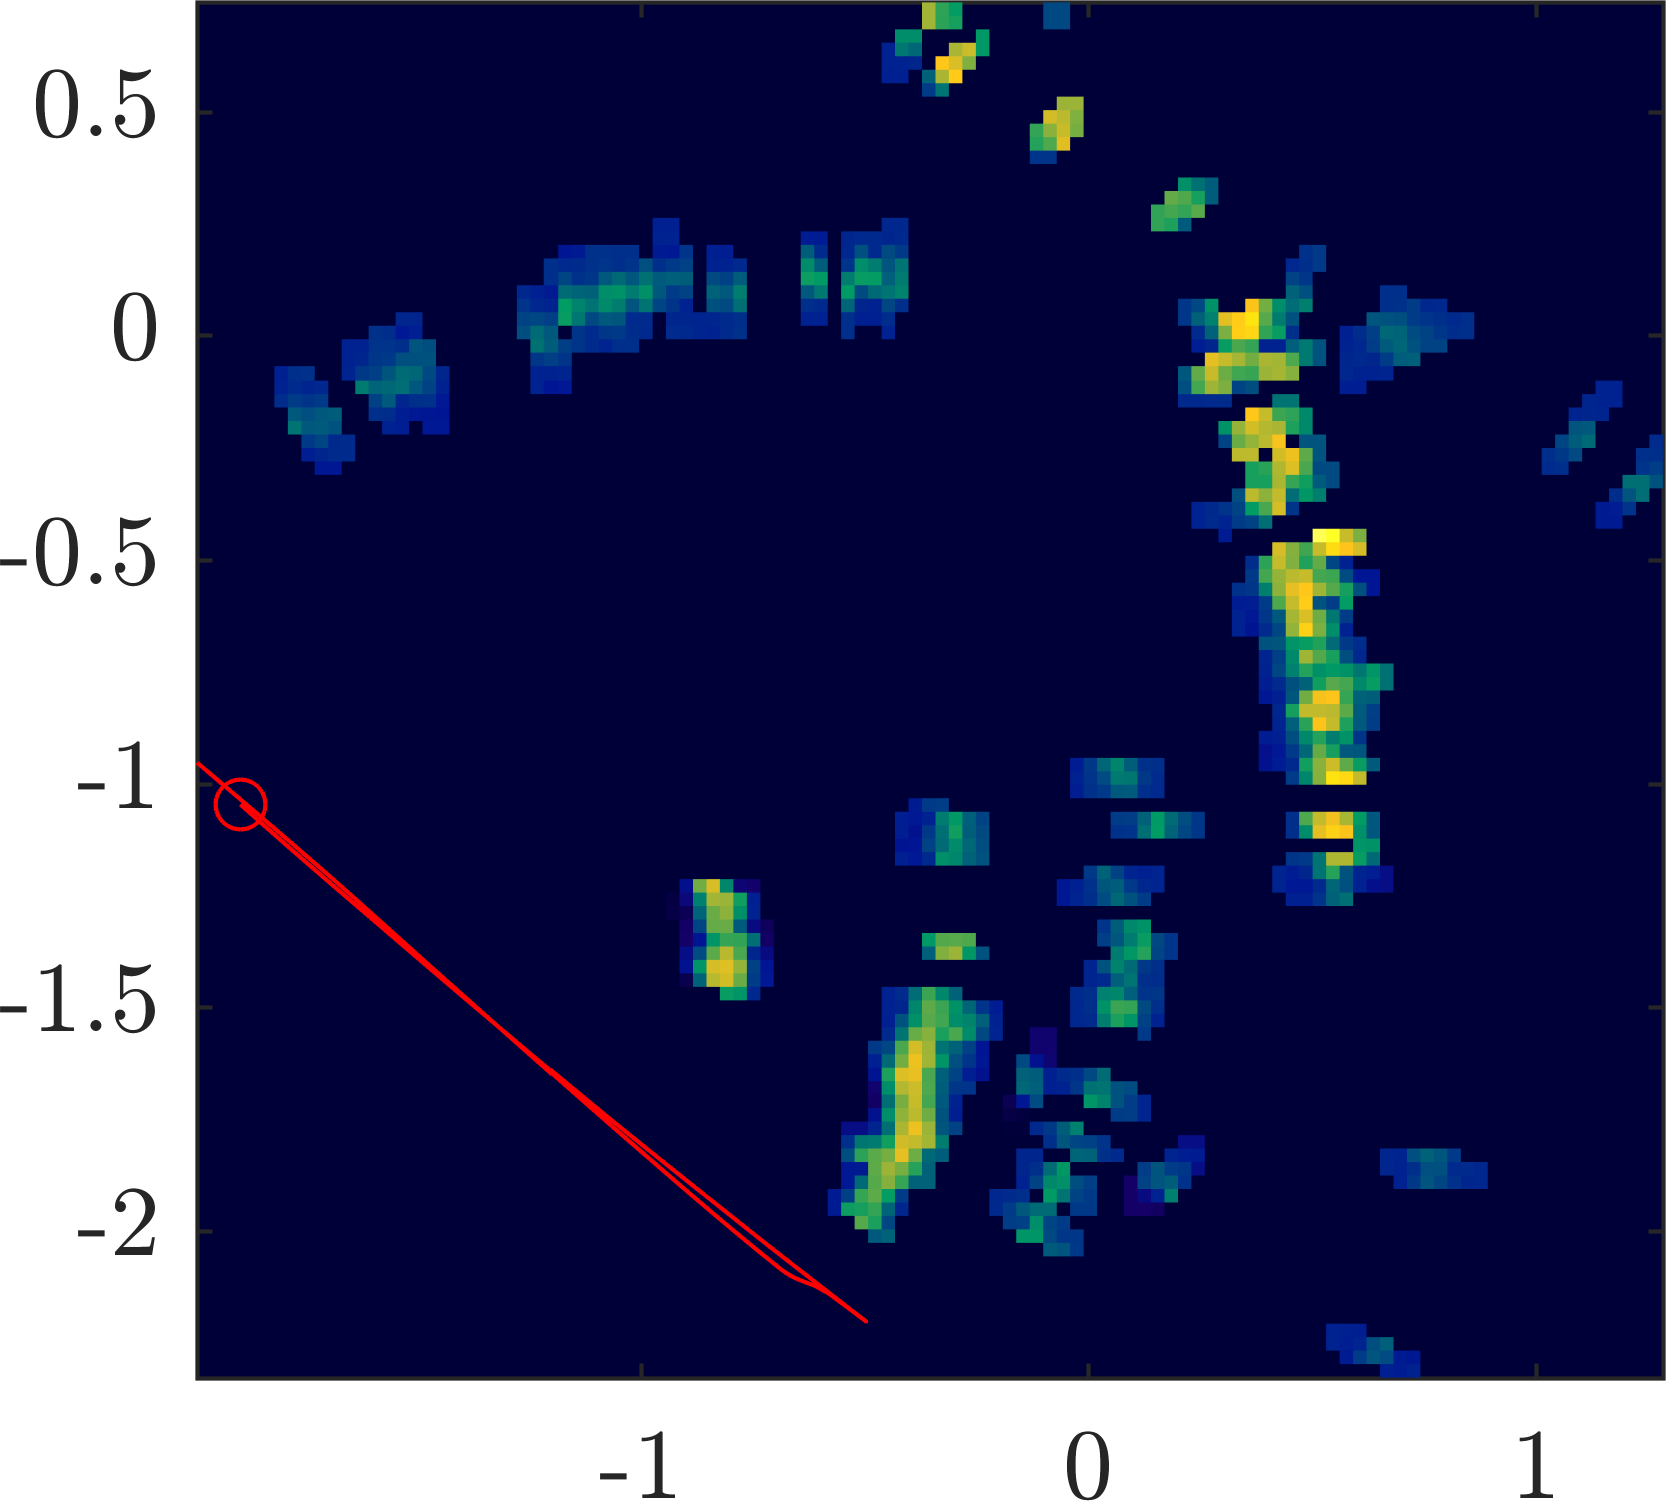
\includegraphics{gfx/results/jailcell_reprojection}}           & 5ms        & H           & 20°    & \cmark & \xmark & \xmark \\
% Kitchen                           & \raisebox{-.5\height}{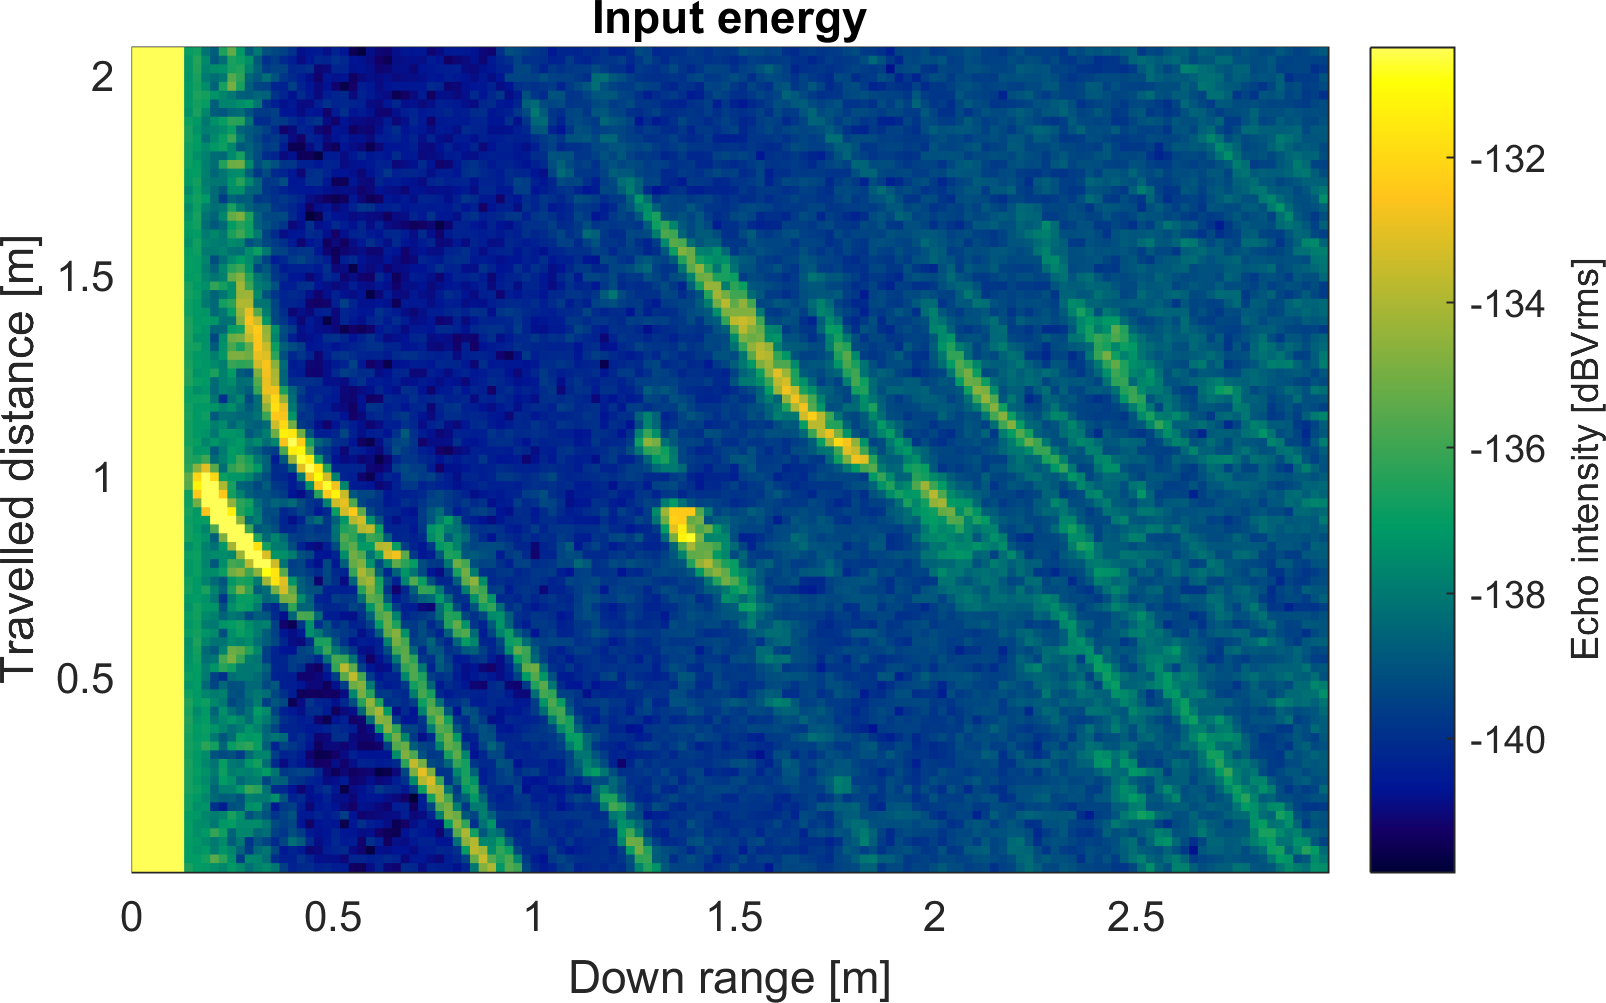
\includegraphics{gfx/results/kitchen_input}}            & \raisebox{-.5\height}{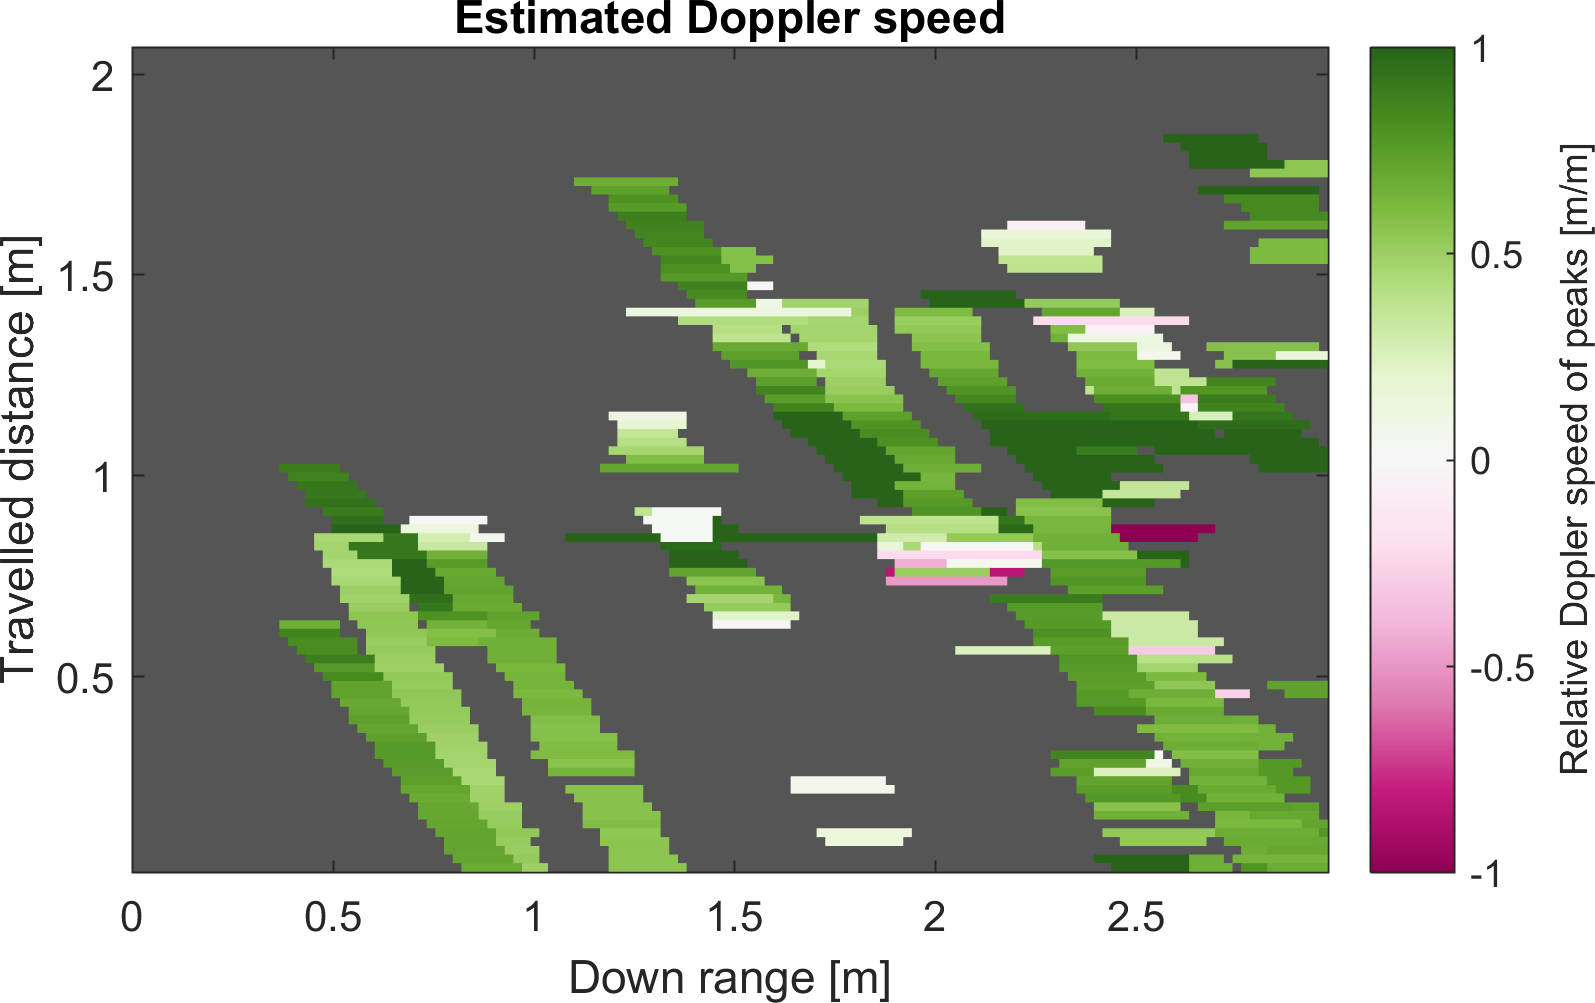
\includegraphics{gfx/results/kitchen_doppler}}            & \raisebox{-.5\height}{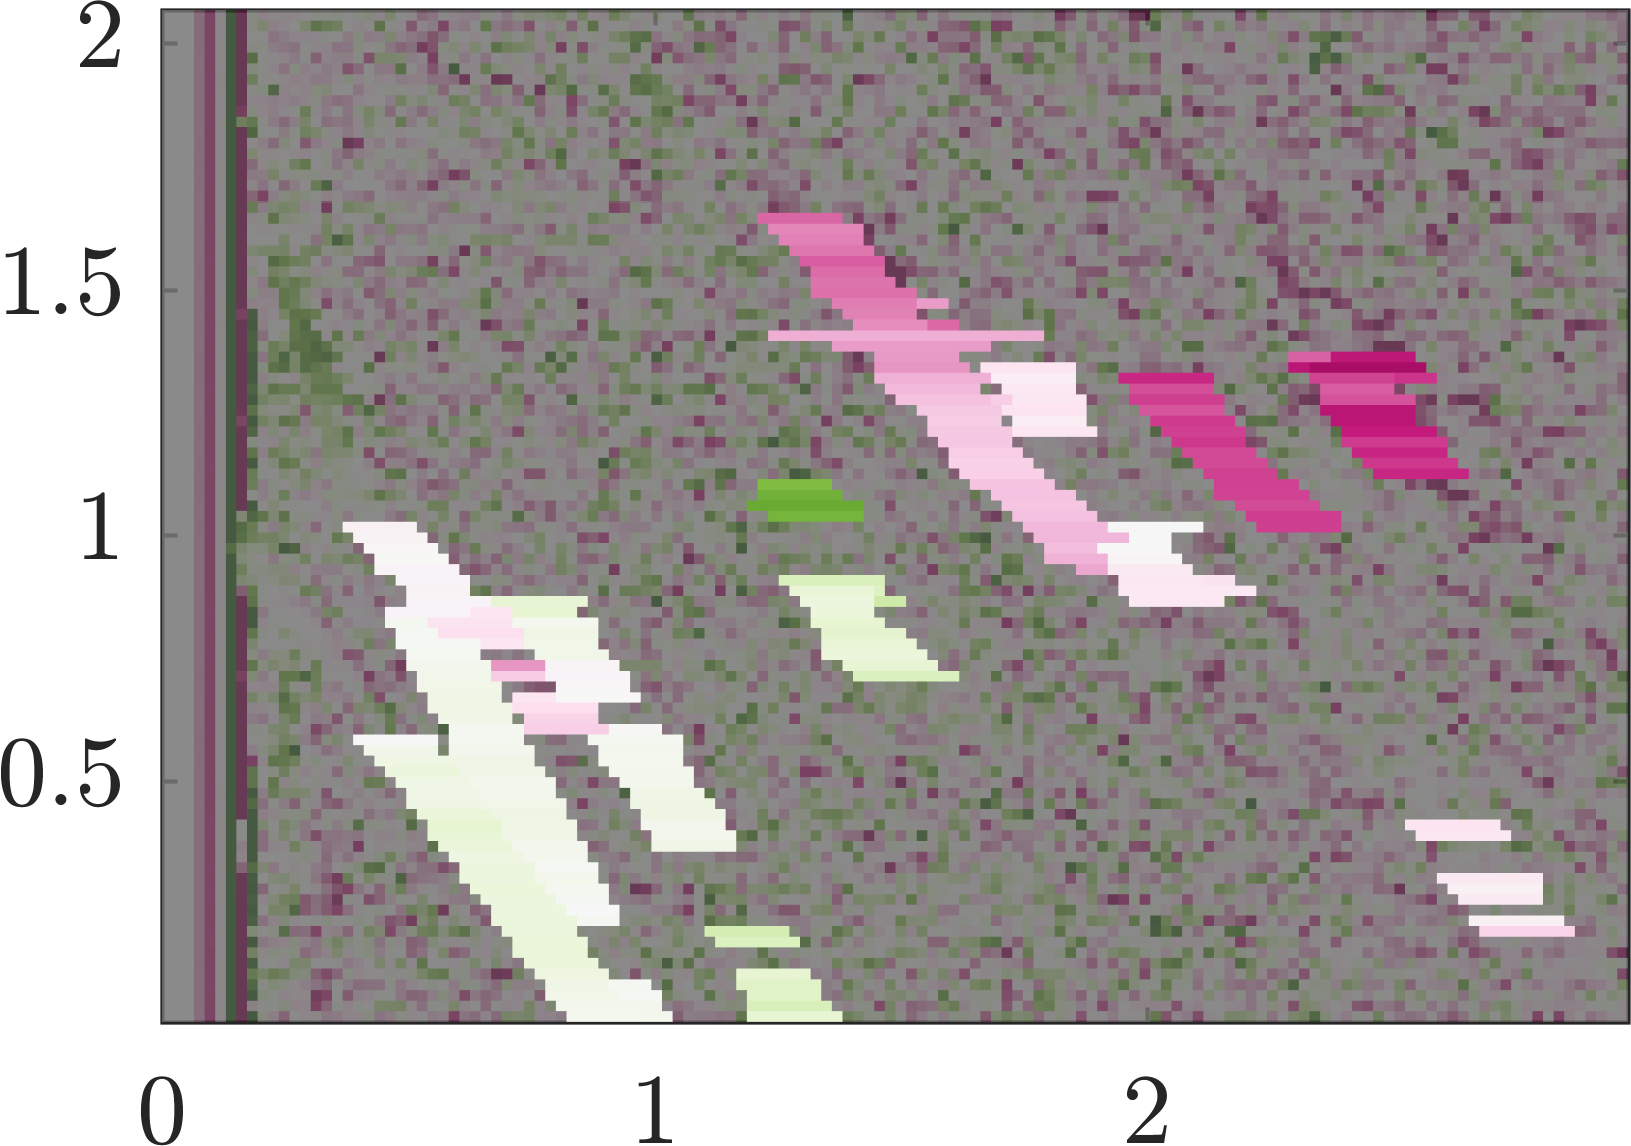
\includegraphics{gfx/results/kitchen_doa}}            & \raisebox{-.5\height}{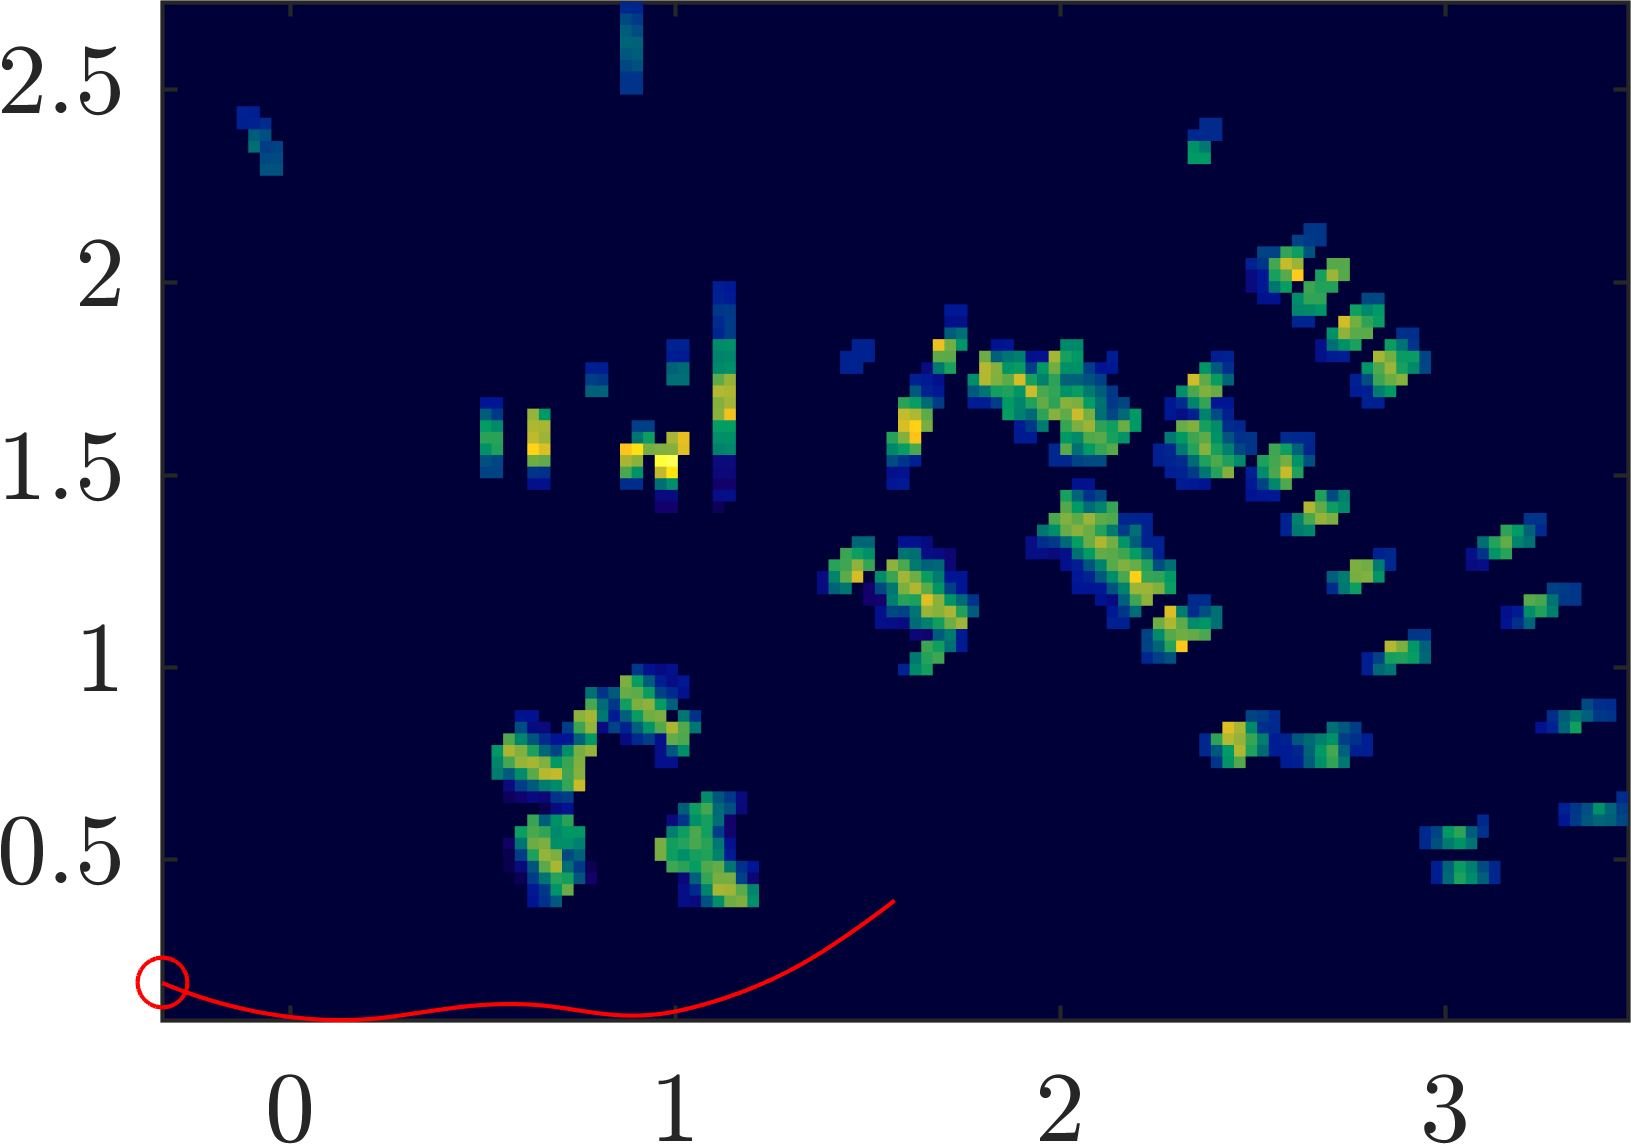
\includegraphics{gfx/results/kitchen_reprojection}}            & 5ms        & H           & 20°    & \xmark & \xmark & \xmark \\
% Lobby                             & \raisebox{-.5\height}{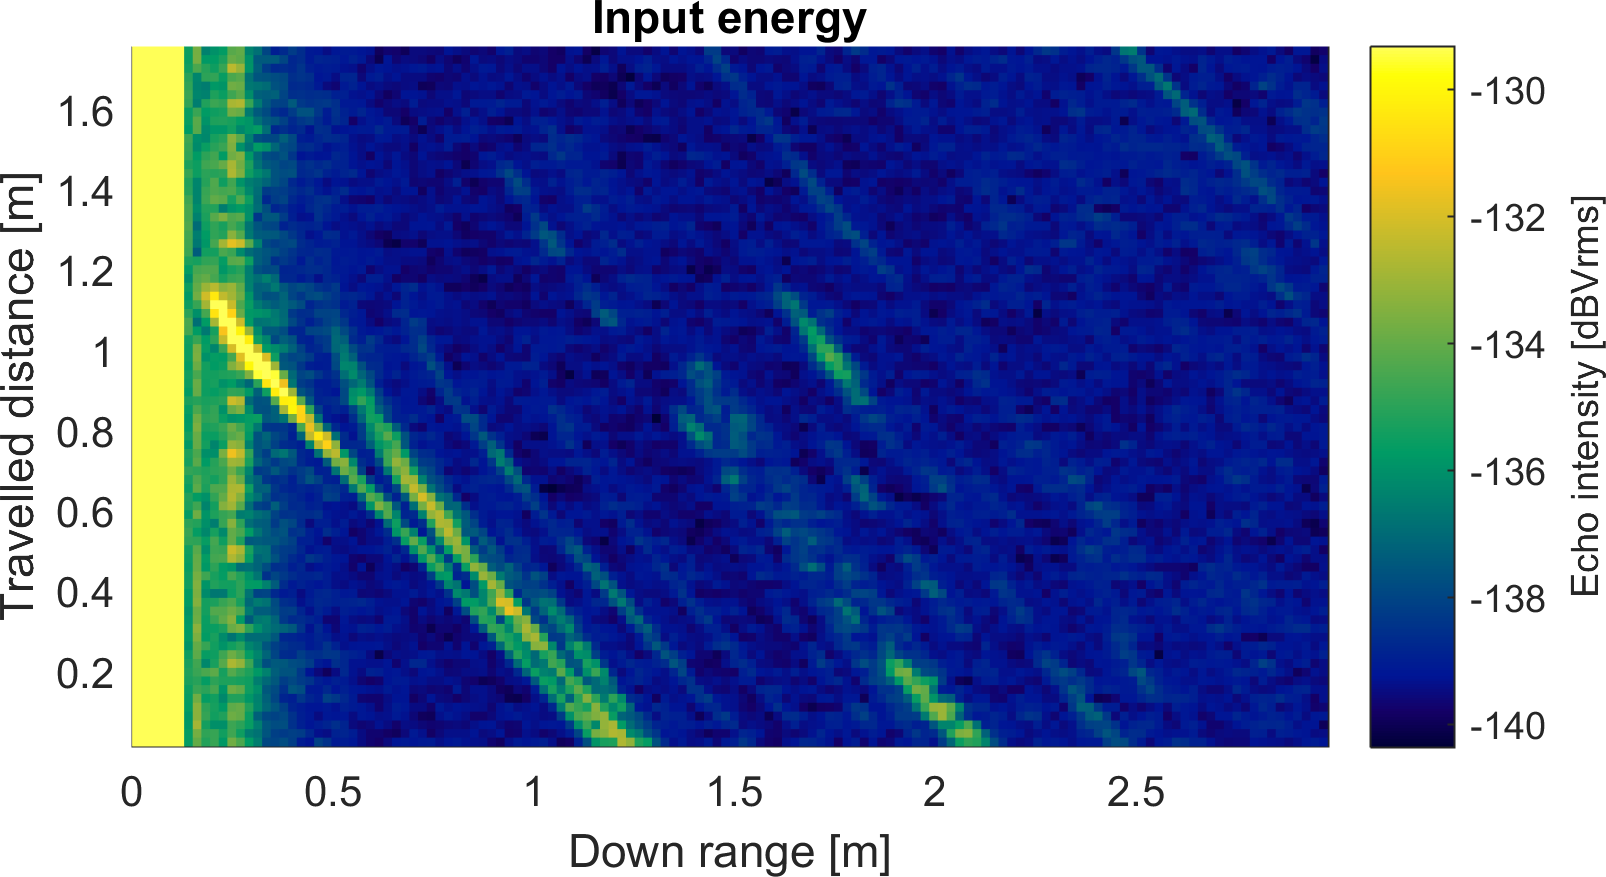
\includegraphics{gfx/results/lobby_input}}              & \raisebox{-.5\height}{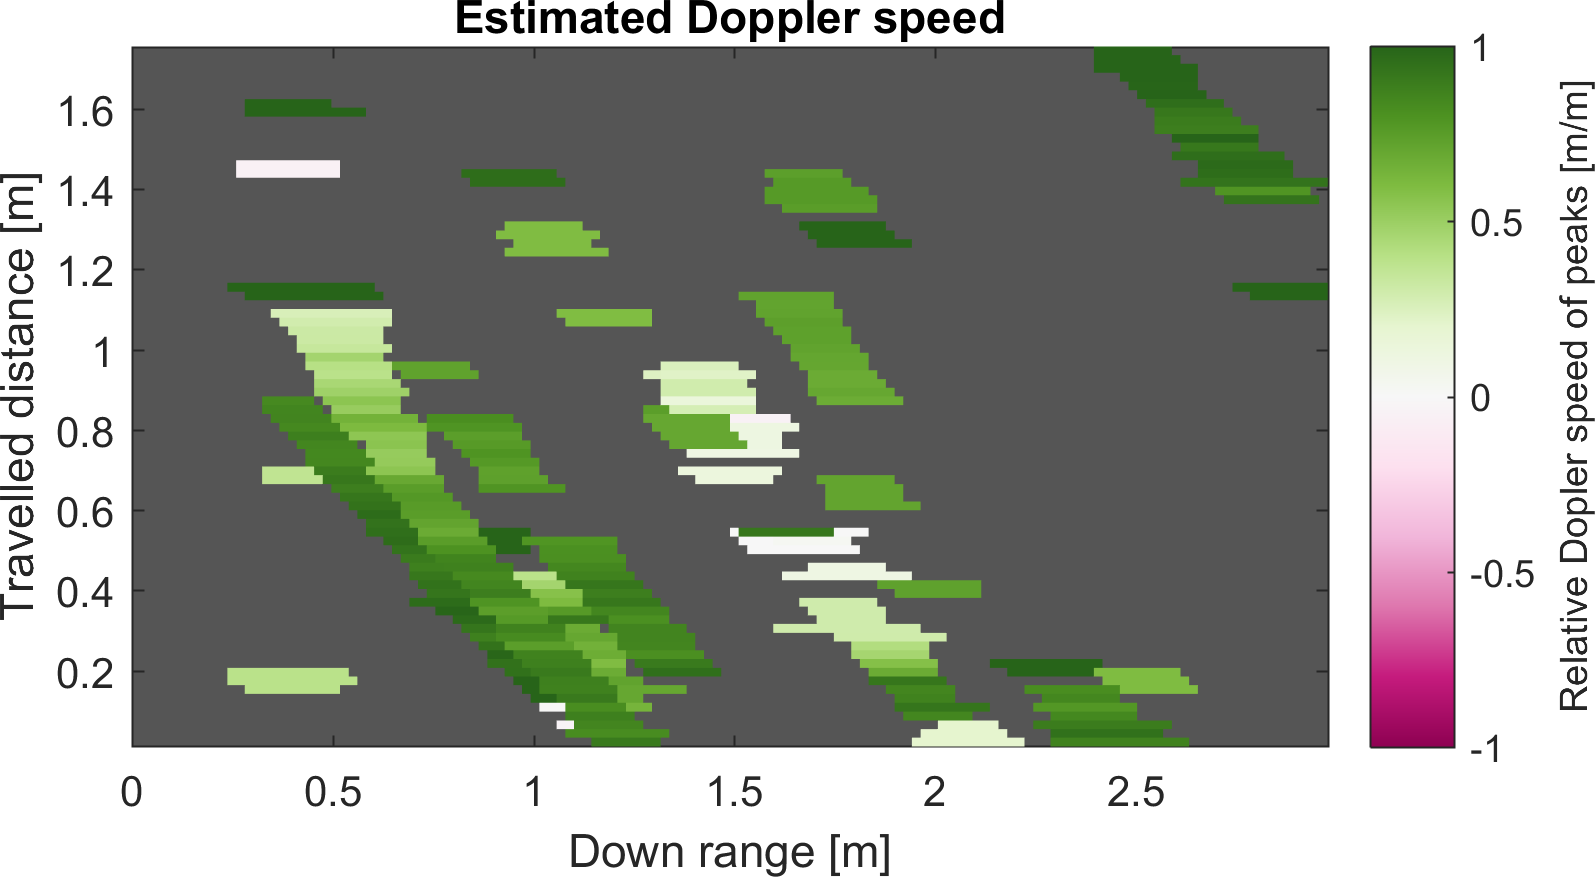
\includegraphics{gfx/results/lobby_doppler}}              & \raisebox{-.5\height}{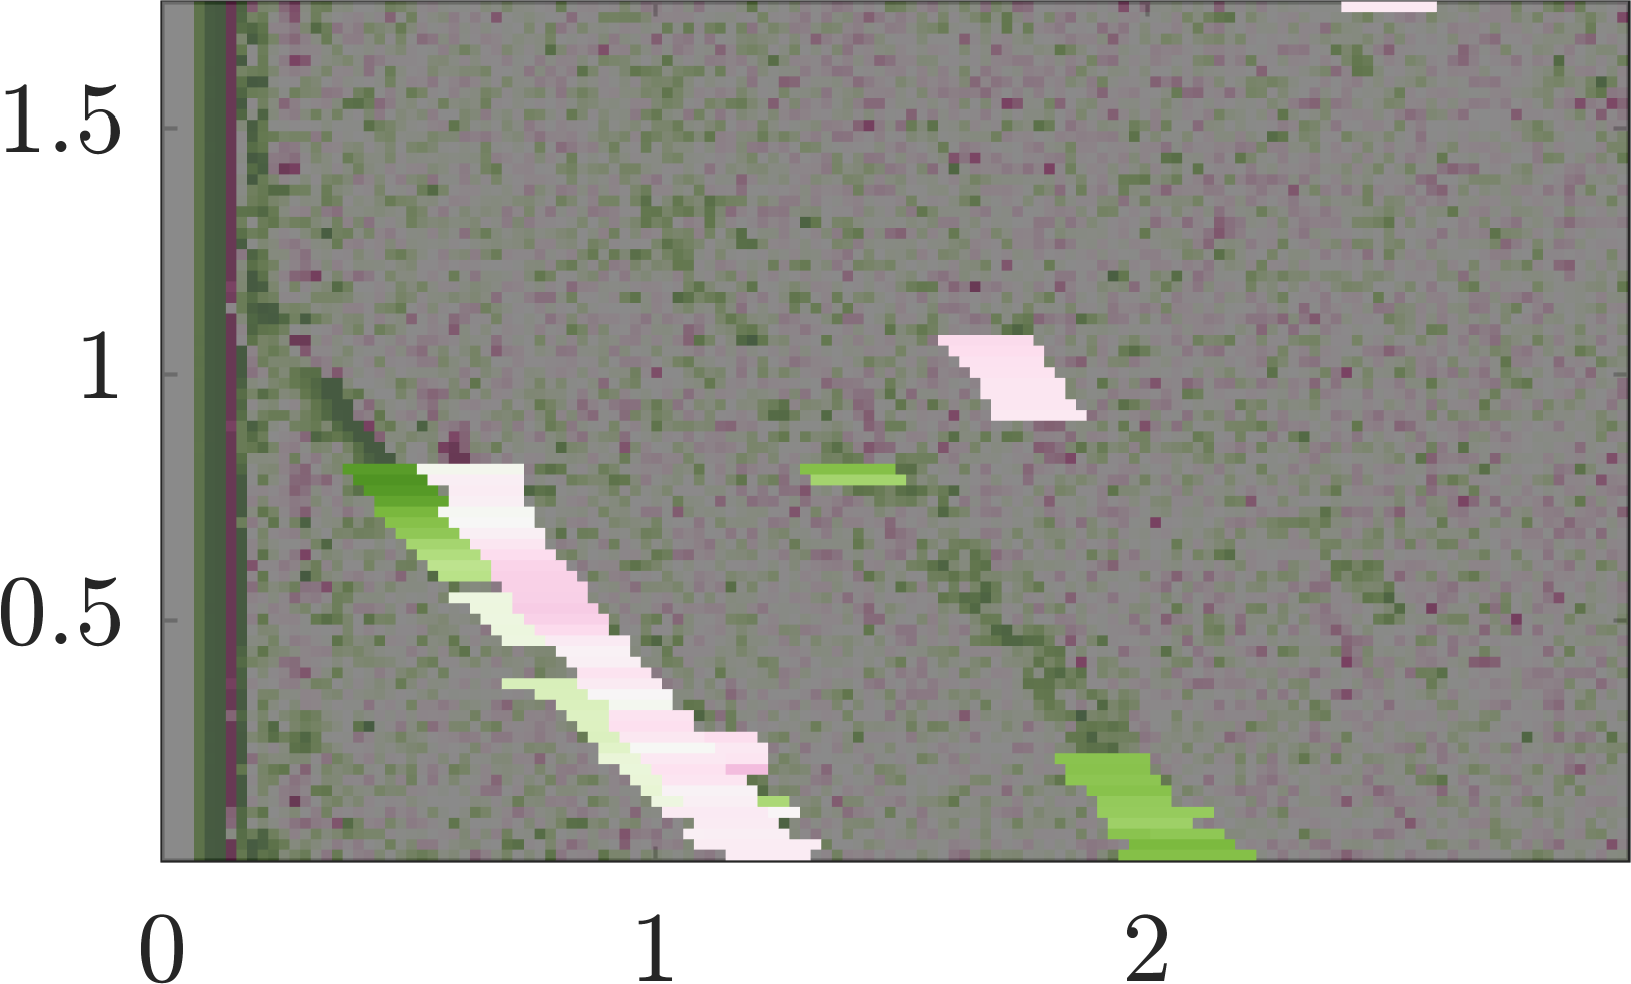
\includegraphics{gfx/results/lobby_doa}}              & \raisebox{-.5\height}{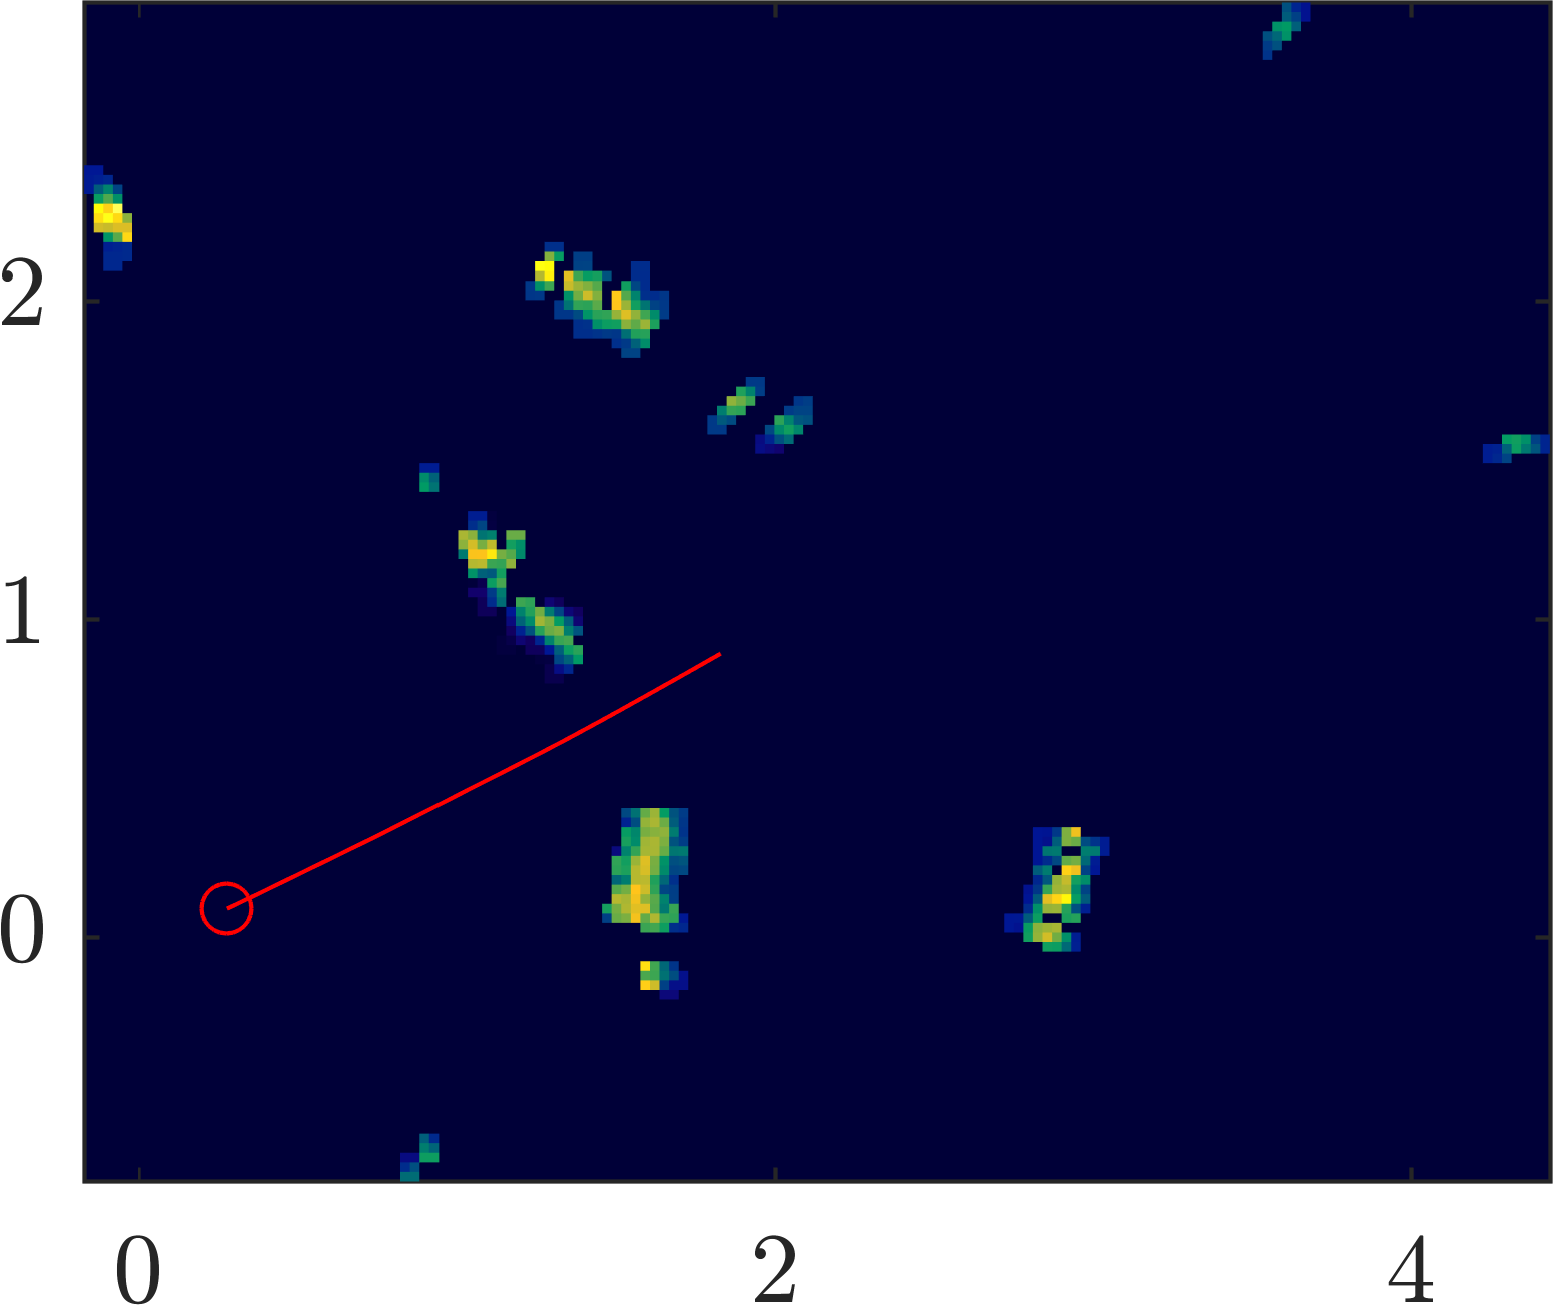
\includegraphics{gfx/results/lobby_reprojection}}              & 5ms        & H/I         & 0°     & \xmark & \xmark & \xmark \\
% Mancave                           & \raisebox{-.5\height}{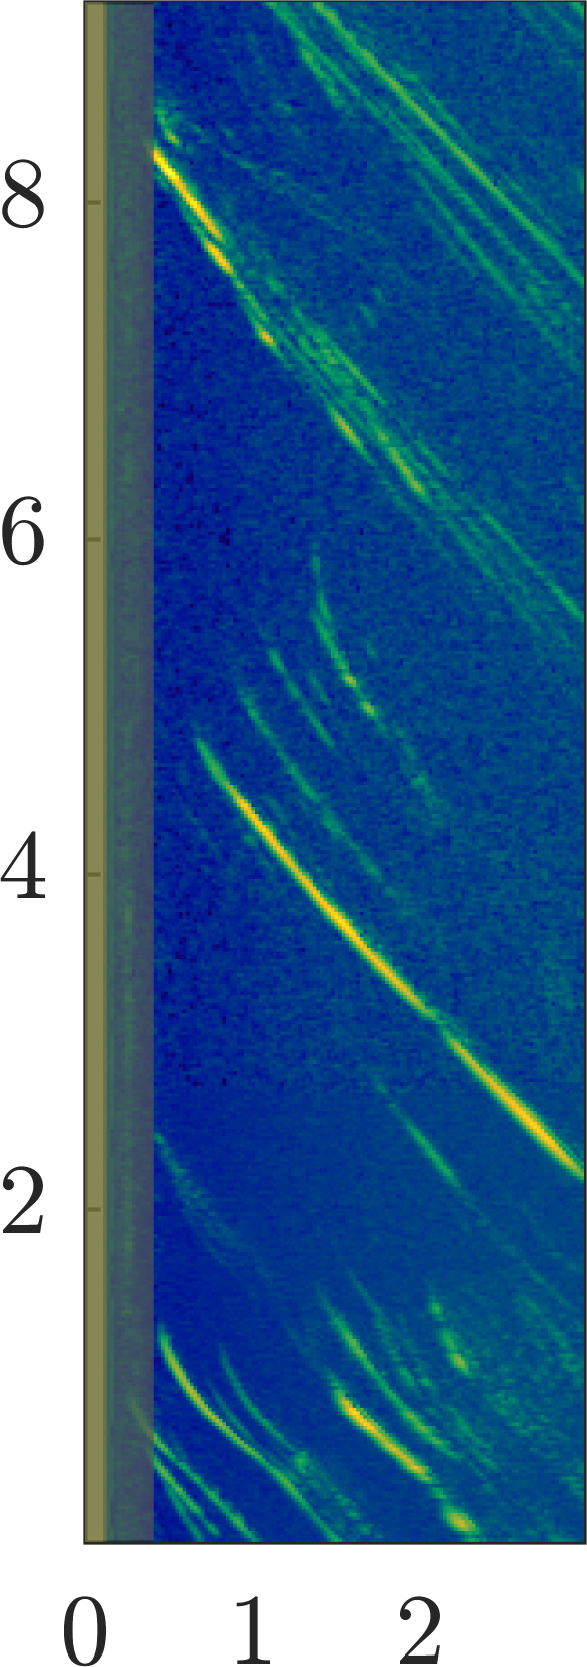
\includegraphics{gfx/results/mancave_input}}            & \raisebox{-.5\height}{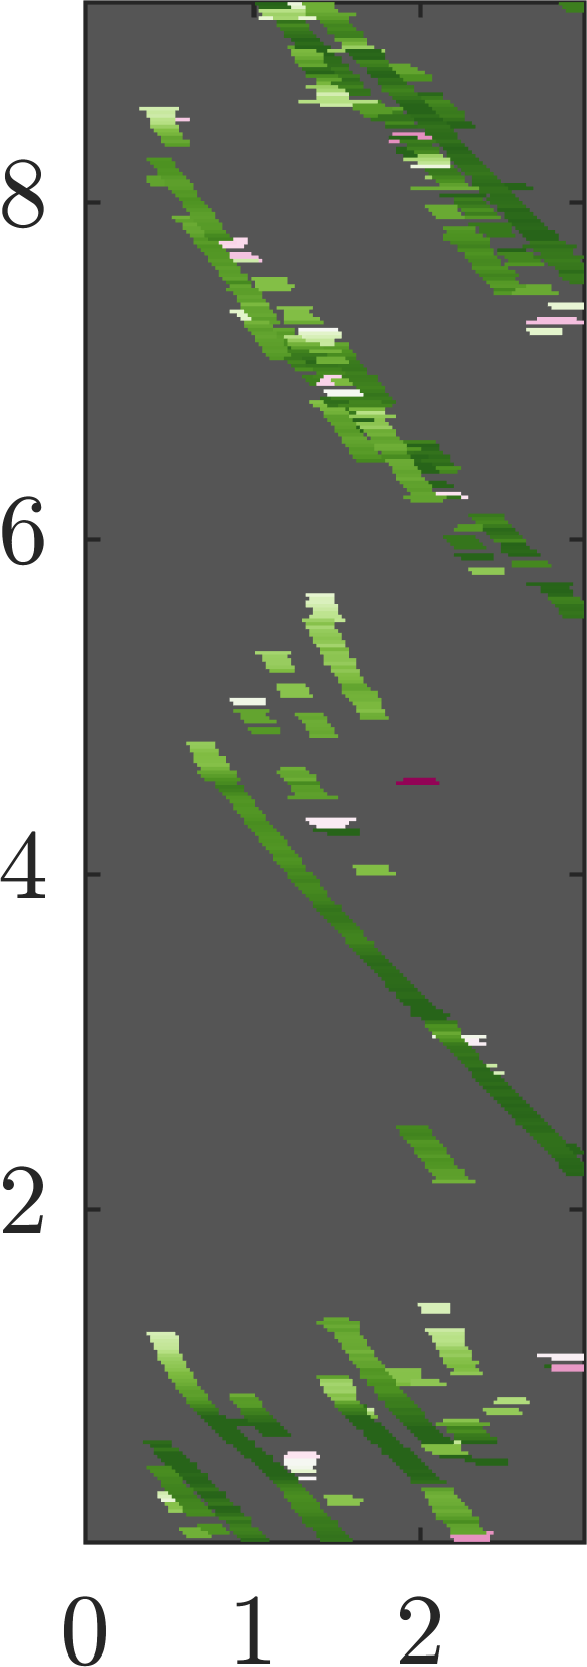
\includegraphics{gfx/results/mancave_doppler}}            & \raisebox{-.5\height}{\includegraphics{gfx/results/mancave_doa}}            & \raisebox{-.5\height}{\includegraphics{gfx/results/mancave_reprojection}}            & 5ms        & H/I         & 0°     & \xmark & \xmark & \xmark \\
% Nirvana                           & \raisebox{-.5\height}{\includegraphics{gfx/results/nirvana_input}}            & \raisebox{-.5\height}{\includegraphics{gfx/results/nirvana_doppler}}            & \raisebox{-.5\height}{\includegraphics{gfx/results/nirvana_doa}}            & \raisebox{-.5\height}{\includegraphics{gfx/results/nirvana_reprojection}}            & 5ms        & H/I         & 0°     & \xmark & \cmark & \xmark \\
% Orbit                             & \raisebox{-.5\height}{\includegraphics{gfx/results/orbit_input}}              & \raisebox{-.5\height}{\includegraphics{gfx/results/orbit_doppler}}              & \raisebox{-.5\height}{\includegraphics{gfx/results/orbit_doa}}              & \raisebox{-.5\height}{\includegraphics{gfx/results/orbit_reprojection}}              & 5ms        & H/I         & 0°     & \xmark & \cmark & \xmark \\
% Public Restroom                   & \raisebox{-.5\height}{\includegraphics{gfx/results/publicrestroom_input}}     & \raisebox{-.5\height}{\includegraphics{gfx/results/publicrestroom_doppler}}     & \raisebox{-.5\height}{\includegraphics{gfx/results/publicrestroom_doa}}     & \raisebox{-.5\height}{\includegraphics{gfx/results/publicrestroom_reprojection}}     & 5ms        & H/I         & 0°     & \xmark & \cmark & \cmark \\
% Queue                             & \raisebox{-.5\height}{\includegraphics{gfx/results/queue_input}}              & \raisebox{-.5\height}{\includegraphics{gfx/results/queue_doppler}}              & \raisebox{-.5\height}{\includegraphics{gfx/results/queue_doa}}              & \raisebox{-.5\height}{\includegraphics{gfx/results/queue_reprojection}}              & 20ms       & H/I         & 0°     & \xmark & \cmark & \cmark \\
% Racetrack                         & \raisebox{-.5\height}{\includegraphics{gfx/results/racetrack_input}}          & \raisebox{-.5\height}{\includegraphics{gfx/results/racetrack_doppler}}          & \raisebox{-.5\height}{\includegraphics{gfx/results/racetrack_doa}}          & \raisebox{-.5\height}{\includegraphics{gfx/results/racetrack_reprojection}}          & 2ms        & H/I         & 0°     & \xmark & \cmark & \cmark \\
% Sauna                             & \raisebox{-.5\height}{\includegraphics{gfx/results/sauna_input}}              & \raisebox{-.5\height}{\includegraphics{gfx/results/sauna_doppler}}              & \raisebox{-.5\height}{\includegraphics{gfx/results/sauna_doa}}              & \raisebox{-.5\height}{\includegraphics{gfx/results/sauna_reprojection}}              & 2.5ms      & H/I         & 0°     & \xmark & \cmark & \cmark \\
% Torture Chamber                   & \raisebox{-.5\height}{\includegraphics{gfx/results/torturechamber_input}}     & \raisebox{-.5\height}{\includegraphics{gfx/results/torturechamber_doppler}}     & \raisebox{-.5\height}{\includegraphics{gfx/results/torturechamber_doa}}     & \raisebox{-.5\height}{\includegraphics{gfx/results/torturechamber_reprojection}}     & 2.5ms      & H/I         & 45°    & \xmark & \cmark & \cmark \\
% Underground                       & \raisebox{-.5\height}{\includegraphics{gfx/results/underground_input}}        & \raisebox{-.5\height}{\includegraphics{gfx/results/underground_doppler}}        & \raisebox{-.5\height}{\includegraphics{gfx/results/underground_doa}}        & \raisebox{-.5\height}{\includegraphics{gfx/results/underground_reprojection}}        & 2.5ms      & H/I         & 45°    & \xmark & \cmark & \cmark \\




\begin{figure}
    % \centering
    \begin{subfigure}[b]{0.25\textwidth}
        \centering
        \includegraphics[width=.9\textwidth]{gfx/results/attic_input.png}
        \caption{\small Input energy}
    \end{subfigure}%
    \begin{subfigure}[b]{0.25\textwidth}  
        \centering 
        \includegraphics[width=.9\textwidth]{gfx/results/attic_doppler.png}
        \caption{\small Doppler estimation}
    \end{subfigure}%
    \begin{subfigure}[b]{0.25\textwidth}   
        \centering 
        \includegraphics[width=.9\textwidth]{gfx/results/attic_doa.png}
        \caption{\small Direction of Arrival}
    \end{subfigure}%
    \begin{subfigure}[b]{0.25\textwidth}   
        \centering 
        \includegraphics[width=.9\textwidth]{gfx/results/attic_reprojection.png}
        \caption{\small Reprojection Map}
    \end{subfigure}%
    \caption{Attic scan}
\end{figure}

\begin{figure}
    % \centering
    \begin{subfigure}[b]{0.25\textwidth}
        \centering
        \includegraphics[width=.9\textwidth]{gfx/results/basement_input.png}
        \caption{\small Input energy}
    \end{subfigure}%
    \begin{subfigure}[b]{0.25\textwidth}  
        \centering 
        \includegraphics[width=.9\textwidth]{gfx/results/basement_doppler.png}
        \caption{\small Doppler estimation}
    \end{subfigure}%
    \begin{subfigure}[b]{0.25\textwidth}   
        \centering 
        \includegraphics[width=.9\textwidth]{gfx/results/basement_doa.png}
        \caption{\small Direction of Arrival}
    \end{subfigure}%
    \begin{subfigure}[b]{0.25\textwidth}   
        \centering 
        \includegraphics[width=.9\textwidth]{gfx/results/basement_reprojection.png}
        \caption{\small Reprojection Map}
    \end{subfigure}%
    \caption{Basement scan}
\end{figure}

TODO



\end{appendix}

\listoffigures
\listoftables

% Index
\clearpage
\printindex

% Literaturverzeichnis
%\nocite{wasauchimmer}
\clearpage
\printbibliography

\end{document}
